%%%%%%%%%%%%%%%%%%%%%%%%%%%%%%%%%%%%%%%%%
% Original author: Harshit Prashant Dhanwalkar
%%%%%%%%%%%%%%%%%%%%%%%%%%%%%%%%%%%%%%%%%

%-------------------------------------------------------------------------------------
%      PACKAGES AND OTHER DOCUMENT CONFIGURATIONS
%-------------------------------------------------------------------------------------

\documentclass[fleqn,10pt]{SelfArx} % Document font size and equations flushed left
\usepackage[english]{babel} 
\usepackage{enumitem}

\usepackage{tikz}
\usetikzlibrary{trees, positioning, shapes}

\usepackage{tikz-3dplot}

\usepackage{amsmath}
\usepackage{array} % for tables

\usepackage{pgfplots}
\pgfplotsset{compat=1.18}

%-------------------------------------------------------------------------------------
%	COLUMNS
%-------------------------------------------------------------------------------------
\setlength{\columnsep}{0.55cm} % Distance between the two columns of text
\setlength{\fboxrule}{0.75pt} % Width of the border around the abstract

%-------------------------------------------------------------------------------------
%	COLORS
%-------------------------------------------------------------------------------------
\definecolor{color1}{RGB}{0,0,90} % Color of the article title and sections
\definecolor{color2}{RGB}{0,20,20} % Color of the boxes behind the abstract and headings

%-------------------------------------------------------------------------------------
%	EQUATIONS
%-------------------------------------------------------------------------------------
\usepackage{cancel} % for crossing the word showing it is cancelled or is zero

%-------------------------------------------------------------------------------------
%	EQUATIONLINKS
%-------------------------------------------------------------------------------------
\newcommand{\myeqref}[1]{\textcolor{blue}{\textup{(\getrefnumber{#1})}}}

%-------------------------------------------------------------------------------------
%	HYPERLINKS
%-------------------------------------------------------------------------------------

\usepackage{xcolor}
\usepackage{hyperref}
\usepackage{footnote}

%\newcommand{\myhref}[2]{\href{#1}{\textcolor{blue}{#2}}}
\newcommand{\myhref}[2]{%
  \href{#1}{\textcolor{blue}{#2}}%
  \footnote{\url{#1}}%
}

\usepackage{cleveref}
% Customize cleveref to use "Eq." for equations
\crefname{equation}{Eq.}{Eq.}
\Crefname{equation}{Eq.}{Eq.}

\hypersetup{
	hidelinks,
	colorlinks,
	breaklinks=true,
	urlcolor=color2,
	citecolor=color1,
	linkcolor=color1,
	bookmarksopen=false,
	pdftitle={Title},
	pdfauthor={Author},
}

% ------------------------------------------------------------------------------------
%       CUSTOM	SYMBOLS
%-------------------------------------------------------------------------------------
\newcommand{\zbar}{\raisebox{0.2ex}{--}\kern-0.6em Z}

%-------------------------------------------------------------------------------------
%	ARTICLE INFORMATION
%-------------------------------------------------------------------------------------
\JournalInfo{Dual Degree Engineering Physics, 7$^{th}$ Semester, 2024} % Journal information
\Archive{Mtech, Earth System Sciences (ESS), 1$^{st}$ year} % Additional notes (e.g. copyright, DOI, review/research article)

\PaperTitle{Lecture Notes on Atmospheric Thermodynamics and Cloud Physics} % Article title

\Authors{Harshit Prashant Dhanwalkar (SC21B164)\textsuperscript{1}*} % Authors
\affiliation{\textsuperscript{1}\textit{MTech, Earth System Sciences (ESS), 1$^{st}$ year, Department of Physics, Indian Institute Of Spacescience and Technology (IIST)}} % Author affiliation
\affiliation{*\textbf{email}: harshitpd1729@gamil.com} % Corresponding author

\Keywords{} % Keywords - if you don't want any simply remove all the text between the curly brackets
\newcommand{\keywordname}{Keywords} % Defines the keywords heading name

%-------------------------------------------------------------------------------------
%	ABSTRACT
%-------------------------------------------------------------------------------------
\Abstract{Notes of Lectures plus addional information from books.}

%-------------------------------------------------------------------------------------
%	DOCUMENT
%-------------------------------------------------------------------------------------
\begin{document}
\maketitle % Output the title and abstract box
\tableofcontents % Output the contents section
\clearpage
\thispagestyle{empty} % Removes page numbering from the first page
\clearpage

%-------------------------------------------------------------------------------------
%	DOCUMENT CONTENTS
%-------------------------------------------------------------------------------------
\section{Lecture 1 09/08/2024} % The \section*{} command stops section numbering

%\addcontentsline{toc}{section}{Introduction} % Adds this section to the table of contents

\begin{itemize}[noitemsep]
    \item System: Specific chunk of matter we are interested in.
    \item Surrounding: Everything else in the universe outside of the system.
    \item Air parcel: System with the following assumptions:
    \begin{itemize}[noitemsep]
        \item Properties within the air parcel are uniform.
        \item Boundaries are closed, so that matter/mass is not exchanged with the surroundings.
    \end{itemize}
\end{itemize}

\begin{question}[label={q:1.1}]{How do system interact with surrounding?}
    \begin{itemize}[noitemsep]
        \item Matter
        \item Radiation
    \end{itemize}
\end{question}

\begin{question}[label={q:1.2}]{Classify system on the basis of how matter interact with surround?}
$\Rightarrow$ We can classify system into 3 types on the basis of how matter in system interact with it's surrounding:

\begin{itemize}[noitemsep]
	\item Open
	\item Closed
	\item Isolated
\end{itemize}
\end{question}

\begin{question}[label={q:1.3}]{How do we characterize a system?}
    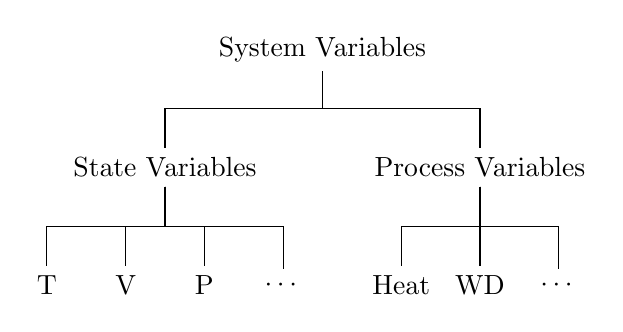
\begin{tikzpicture}[edge from parent fork down, sibling distance=2cm, level 1/.style={sibling distance=4cm}, level 2/.style={sibling distance=1cm}]
        % Define the tree structure
        \node {System Variables}
            child { node {State Variables}
                child { node {T} }
                child { node {V} }
                child { node {P} }
                child { node {$\cdots$}}
            }
            child { node {Process Variables}
                child { node {Heat} }
                child { node {WD} }
                child { node {$\cdots$}}
            };
    \end{tikzpicture}

    such that: $f(V,P,T)=0 \rightarrow \text{equation of state}$
\end{question}

\subsection{Equilibrium State}
Equilibrium: No change in the system if the surrounding doesn't change.

\begin{tikzpicture}[edge from parent fork down, sibling distance=1cm, level 1/.style={sibling distance=2.5cm}, level 2/.style={sibling distance=0.5cm}]
    % Define the tree structure
    \node {Equilibrium States}
        child { node {Stable Eq.}
            child { node {
                \begin{tikzpicture}
                    \begin{axis}[
                        width=3cm,
                        height=3cm,
                        axis lines=middle,
                        xlabel={$x$},
                        ylabel={$y$},
                        xmin=-2, xmax=2,
                        ymin=-1, ymax=5,
                        domain=-2:2,
                        samples=50,
                        every axis label/.append style={font=\tiny},
                        every tick label/.append style={font=\tiny},
                    ]
                        \addplot[blue, thick] {x^2};
                        \addplot[mark=*, mark options={scale=0.7, color=black}] coordinates {(0,0.3)};
                    \end{axis}
                \end{tikzpicture}
            }   }
        }
        child { node {Unstable Eq.}
            child { node {
                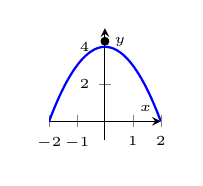
\begin{tikzpicture}
                    \begin{axis}[
                        width=3cm,
                        height=3cm,
                        axis lines=middle,
                        xlabel={$x$},
                        ylabel={$y$},
                        xmin=-2, xmax=2,
                        ymin=-1, ymax=5,
                        domain=-2:2,
                        samples=50,
                        every axis label/.append style={font=\tiny},
                        every tick label/.append style={font=\tiny},
                    ]
                        \addplot[blue, thick] {-x^2 + 4};
                        \addplot[mark=*, mark options={scale=0.7, color=black}] coordinates {(0,4.3)};
                    \end{axis}
                \end{tikzpicture}
            }   }
        }
        child { node {Metastable Eq.}
            child { node {
                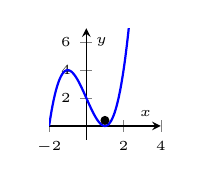
\begin{tikzpicture}
                    \begin{axis}[
                        width=3cm,
                        height=3cm,
                        axis lines=middle,
                        xlabel={$x$},
                        ylabel={$y$},
                        xmin=-2, xmax=4,
                        ymin=-1, ymax=7,
                        domain=-2:4,
                        samples=100,
                        every axis label/.append style={font=\tiny},
                        every tick label/.append style={font=\tiny},
                    ]
                        \addplot[blue, thick] {x^3 - 3*x + 2};
                        \addplot[mark=*, mark options={scale=0.7, color=black}] coordinates {(1,0.4)};
                    \end{axis}
                \end{tikzpicture}
            }   }
        };
\end{tikzpicture}

%\begin{tikzpicture}[
%    edge from parent fork down, 
%    sibling distance=1cm, % Distance between sibling nodes
%    level 1/.style={sibling distance=3cm}, % Distance between Level 1 nodes
%    level 2/.style={sibling distance=1.5cm}, % Distance between Level 2 nodes
%    every node/.style={font=\small, text centered}
%]
    % Define the tree structure
%    \node {Equilibrium State}
%        child { node {Stable Eq.} }
%        child { node {Unstable} }
%        child { node {Metastable} };
%\end{tikzpicture}

\subsection{Transformation}
\begin{center}
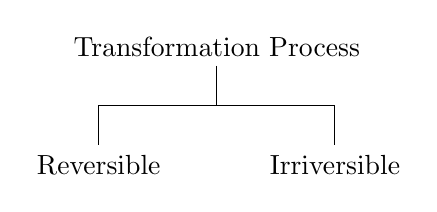
\begin{tikzpicture}[edge from parent fork down, sibling distance=1.5cm, level 1/.style={sibling distance=3cm}, level 2/.style={sibling distance=1.5cm}]
% Define the tree structure
\node {Transformation Process}
    child { node {Reversible}}
    child { node {Irriversible}};
\end{tikzpicture}
\end{center}

% TODO: ADD PLOT FOR REVERSIBLE PROCESS, with ref
\begin{figure}[ht]
    \begin{center}
        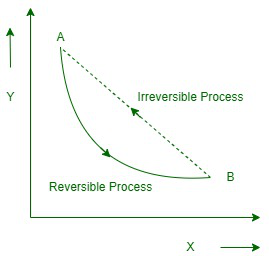
\includegraphics[width=0.25\textwidth]{Figures/Rev_irr_process.jpg}
    \end{center}
    \caption{Reversible and Irreversible Process}\label{fig:Rev_irr_process}
\end{figure}

\subsection{Exact and Inexact differentiable}
Let $z$ be a function of $x$ and $y$, exact differentuable equation:
\begin{align}
    dz &= \left(\frac{\partial z}{\partial x}\right) dx + \left(\frac{\partial z}{\partial y}\right) dy \\
    dz &= \int_i^f \delta z = z(x_f,y_f) - z(x_i,y_i)
\end{align}

$\therefore$ $dT,dP,dV$ are exact diffferenrtiable.

$\delta Q, \delta W$ are inexact diffferenrtiable.

line intregral:
$$
\oint \delta z = 0
$$
$\rightarrow$ $z$ is stable variable and it is exact differentiable iff it's reversible

$$
\therefore \oint dT = 0, \oint dP = 0, \oint dq \neq 0, \oint dw \neq 0 
$$

\subsection{Exntensive and Intrincive variables}
\begin{itemize}[noitemsep]
    \item \textbf{Entrisive}: Depends on size of system. E.g. Volume.
    \item \textbf{Intrincive}: Independent of size of system. E.g. Temperature.
\end{itemize}

Any variable divided by mass gives intrincive.

For e.g. specific volume ($\alpha) = \frac{volume}{mass}$.

Similiarly, $$p = \frac{P}{m}, q = \frac{Q}{m}, w = \frac{W}{m}$$

\subsection{Laws of Thermodynamics}
\begin{enumerate}
    \item $0^\text{th}$ law of thermodynamics:

    \textbf{Temperature} $\rightarrow$ Quantity that determines the direction of heat flow. If two objects are in thermal contact and there is no net heat transfer, then the system is said to be in \textbf{thermal equilibrium}.
\end{enumerate}

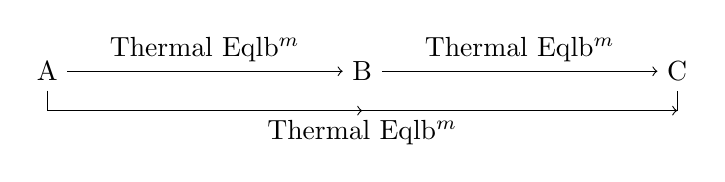
\begin{tikzpicture}
    \node (A) at (0,0) {A};
    \node (B) at (4,0) {B};
    \node (C) at (8,0) {C};

    \draw[->] (A) -- (B);
    \draw[->] (B) -- (C);
    \draw (A) -- (0,-0.5);
    \draw[->] (0,-0.5) -- (4,-0.5);
    \draw[->] (4,-0.5) -- (8,-0.5);
    \draw (8,-0.5) -- (C);
%    \draw[->] (0,-0.5) -- (4,-0.5);

    \node[above] at (2,0){Thermal Eqlb$^m$};
    \node[above] at (6,0){Thermal Eqlb$^m$};
    \node[below] at (4,-0.5){Thermal Eqlb$^m$};
\end{tikzpicture}

% NOTE: COMPLETED L-1
%-------------------------------------------------------------------------------------
\clearpage
\section{Lecture 2 14/08/2024}

Bulk properties $\rightarrow$ microscopic properties $\rightarrow$ which can be linked to microscopic properties

For e.g. $P$ is exerted due to random motion and colllion of moleules with each other and on the walls of container.

\subsection{Kinetic molecular therory of gases}
Conditions:
\begin{itemize}[noitemsep]
        \item Molecules are in \textbf{random motion}.
        \item Collions between molecules with each other and wall of container are \textbf{elastic} in nature ensuring \textbf{no K.E. loss}.
\end{itemize}

\subsubsection*{Derivation of av. K.E.}
Particles travels distance equal to lenght of box ($L$) with velocity $V_x, V_y \text{ and } V_z$.

\begin{tikzpicture}
    [tdplot_main_coords,
    grid/.style={very thin,gray},
    axis/.style={->,blue,thick},
    cube/.style={opacity=.5,very thick}, scale=1]

    % Draw the bottom of the cube first
    \draw[cube,fill=gray!80] (0,0,0) -- (0,2,0) -- (2,2,0) -- (2,0,0) -- cycle;

    % Draw the grid on the bottom (in front of the cube bottom face)
    \foreach \x in {-0.5,0,...,2.5} {
        \draw[grid] (-0.5, -\y, \x) -- (2.5, -\y, \x);
    }
    \foreach \y in {-0.5,0,...,2.5} {
        \draw[grid] (\y, -\x, -0.5) -- (\y, -\x, 2.5);
    }

    % Draw the back-right of the cube
    \draw[cube,fill=gray!80] (0,0,0) -- (0,2,0) -- (0,2,2) -- (0,0,2) -- cycle;

    % Draw the back-left of the cube
    \draw[cube,fill=gray!80] (0,0,0) -- (2,0,0) -- (2,0,2) -- (0,0,2) -- cycle;

    % Draw the front-right of the cube
    \draw[cube] (2,0,0) -- (2,2,0) -- (2,2,2) -- (2,0,2) -- cycle;

    % Draw the front-left of the cube
    \draw[cube] (0,2,0) -- (2,2,0) -- (2,2,2) -- (0,2,2) -- cycle;

    % Draw the top of the cube
    \draw[cube] (0,0,2) -- (0,2,2) -- (2,2,2) -- (2,0,2) -- cycle;

    % Draw particle
    \filldraw[red] (0,1,1) circle (2.3pt) node[anchor=east] {Particle};
    \filldraw[red] (2,1,1) node[anchor=west] {elastic collision};

    % Draw motion arrows
    \draw[->, thick, blue] (0.1,1,1.05) -- (2,1,1.05);
    \draw[->, thick, blue] (2,1,0.85) -- (0.1,1,0.85);

    %velocity arrows
    \draw[->, thick, black] (0.6,0.6,0.5) -- (1.2,0.6,0.5);
    \draw[->, thick, black] (1.2,1,0.5) -- (0.6,1,0.5);

    % Axis labels
    \draw[thick,->] (-0.5,0,0) -- (2.5,0,0) node[right] {$x$};
    \draw[thick,->] (0,-0.5,0) -- (0,2.5,0) node[above] {$z$};
    \draw[thick,->] (0,0,-0.5) -- (0,0,2.5) node[below left] {$y$};

    % Cube length label
    \node at (1, -0.5, 1.4) {L};
    \node at (1, 0.4, 0.5) {$v_x$};
    \node at (1, 1.2, 0.5) {$-v_x$};
\end{tikzpicture}

Force excerted by the molecules  on the face:
\begin{equation}
   F = \frac{\Delta P}{\Delta t} = \frac{\Delta mv}{\Delta t} = m\frac{\Delta v}{\Delta t}
    \label{eq:force exerted}
\end{equation}

Change in velocity 
\begin{align}
   \Delta v_x &= v_x - (-v_x) = 2v_x \\
   \Delta v_y &= 0 \\
   \Delta v_z &= 0 \\
   \implies \Delta V &= 2v_x
   \label{eq:velocity of particle}
\end{align}
\begin{align}
    \therefore F = \frac{m (2v_x)}{\Delta t}     \label{eq: force_equation}
\end{align}

We also have,
\begin{equation}
    \Delta t = \frac{2L}{v_x}
    \label{eq: time_equation}
\end{equation}

from \cref{eq: force_equation} and \cref{eq: time_equation}, we get:
\begin{equation}
    F = \frac{m (2v_x^2)}{2L} = \frac{m v_x^2}{L}
\end{equation}

For $N$ number of molecules and average velocity of all molecules moving in $x$-direction $\bar{v}_x$
\begin{equation}
    \therefore F = \frac{Nm (\bar{v}_x^2)}{L}
\end{equation}

Pressure (P) exerted on walls of container:
\begin{align}
    P &= \frac{F}{A} = \frac{Nm (\bar{v}_x^2)}{L \times L^2} = \frac{Nm (\bar{v}_x^2)}{V} \\
    \implies  PV &=  Nm (\bar{v}_x^2)
\end{align}

When we consider  the velocity of molecules in all directions $(v_{tot})$.
\begin{align}
    v_{tot}^2 &= \bar{v}_x^2 + \bar{v}_y^2 + \bar{v}_z^2 \\
    \implies \bar{v}_{tot}^2 &= 3\bar{v}_x^2
\end{align}

$\therefore$ The Pressue(P) becomes:
\begin{align}
    PV &= \frac{1}{3} Nm \bar{v}_{tot}^2 \\
    3PV &= Nm \bar{v}_{tot}^2 \\
    \frac{3}{2} PV &= \frac{1}{2} Nm \bar{v}_{tot}^2 \\
    \frac{3}{2} PV &= N \times \Big(\frac{1}{2}m\bar{v}_{tot}^2 \Big)\\ 
    \implies \frac{3}{2} PV &= N \times(K.E.)_{av}\\ 
\end{align}

Using Ideal gas equation : $PV=Nk_BT$,\\ where $k_B$ is boltzman constant 
\begin{align}
   \frac{3}{2} (Nk_BT) &= N \times(K.E.)_{av}\\ 
   \implies (K.E.)_{av}&= \frac{3}{2} k_BT
\end{align}

\subsection{Ideal gas}
\begin{enumerate}[noitemsep]
    \item Molcules are in random motion. 
    \item During the motion of \textbf{molecules do not exert force, except when they collide with each other or the walls of container}. This can also be stated as there is \textbf{no force of attraction between mocecules}.
    \item The collisions between molecules are \textbf{elastic}.
    \item \textbf{Sum of the volume of molecules is negligible} comapered to volume of container.
\end{enumerate}

\subsection{Early experiments and laws}
\subsubsection*{$1^{st}$ Law of Gay-Lussac}
Increase of volume of an ideal gas at \textbf{constant pressure} is proportional to incrase in temperature and also to the volume occupied by the gas at $0^o$C

\begin{align}
    dV &\propto V_0 d\theta \\
    dV &= \alpha V_0 d\theta
\end{align}

where $\alpha$ is volume coeffient of thermal expansion.
\begin{align}
    \alpha &= \frac{1}{d \theta} \frac{dV}{V_0} = \frac{1}{273} \\
    \int_{V_0}^{V} dV &= \int_{0^oC}^{\theta} \alpha V_0 d\theta \\
    V - V_0 &= \alpha V_0(\theta - 0^oC) \\
    \Rightarrow V &= (1+\alpha\theta)V_0
\end{align}

\begin{figure}
    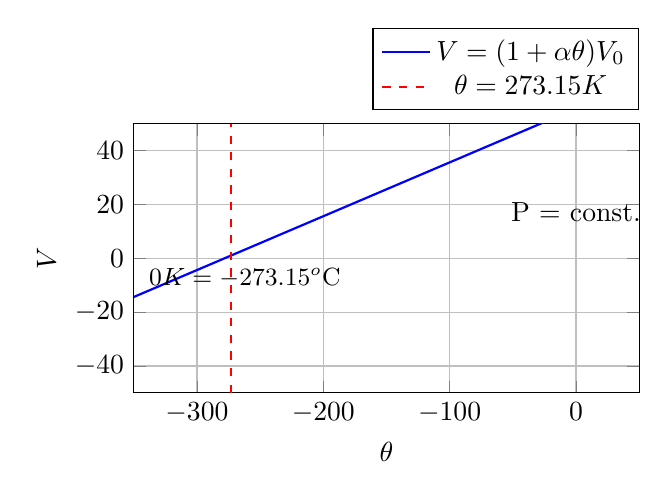
\begin{tikzpicture}
        \begin{axis}[
            xlabel={$ \theta $},
            ylabel={$ V $},
            xmin=-350, xmax=50,
            ymin=-50, ymax=50,
            domain=-350:50,
            grid=both,
            width=8cm, % Adjust width as needed
            height=5cm, % Adjust height as needed
            legend style={at={(1,1.05)}, anchor=south east},
            ]

            % Plot for v = (1 + alpha * theta) * v0 for positive y-axis
            \addplot[
                thick,
                blue,
                label={$V = (1+\alpha\theta)V_0$}
            ] {((1 + 0.2*(x + 273.15)))};

            % Vertical line x = 273.15
            \addplot[
                thick,
                red,
                dashed,
                label={$x = -273.15$}
            ] coordinates {(-273.15, -50) (-273.15, 50)};

            % Labels and annotations
            \node[anchor=north] at (axis cs:-262.15,0) {\small{$0 K = -273.15^o$C}};
            \node[anchor=south] at (axis cs:0,10) {P = const.};

            % Legend
            \addlegendentry{$V = (1+\alpha\theta)V_0$}
            \addlegendentry{$\theta = 273.15K$}
        \end{axis}
    \end{tikzpicture}
    \caption{Plot of $V$ vs. $\theta$}
\end{figure}

\subsubsection*{$2^{st}$ Law of Gay-Lussac}
An Ideal gas kept at constant volume, then the increase in pressure is proportional to increase in termperature and pressure at $0^o$C.

\begin{align}
    dP &\propto P_0 d\theta \\
    dP &= \beta P_0 d\theta
\end{align}

where $\beta$ is pressure coeffient of thermal expansion.
\begin{align}
    \beta &= \frac{1}{d \theta} \frac{dP}{P_0} = \frac{1}{273} \\
    \int_{P_0}^{P} dP &= \int_{0^oC}^{\theta} \beta P_0 d\theta \\
    P - V_0 &= \beta P_0(\theta - 0^oC) \\
    \Rightarrow P &= (1+\beta\theta)P_0
\end{align}

% NOTE: COMPLETED L-2
% ------------------------------------------------------------------------------------
\clearpage

\section{Lecture 3 16/08/2024}

\begin{question}[label={q:3.1}]{Why do  we need Kinetic theory of gases?}
	$\Rightarrow$ Kinetic therory of gases connects microscopic properties to macroscopic properties of gases.
\end{question}

\subsection{Another form of Gay-Lussac's Law}

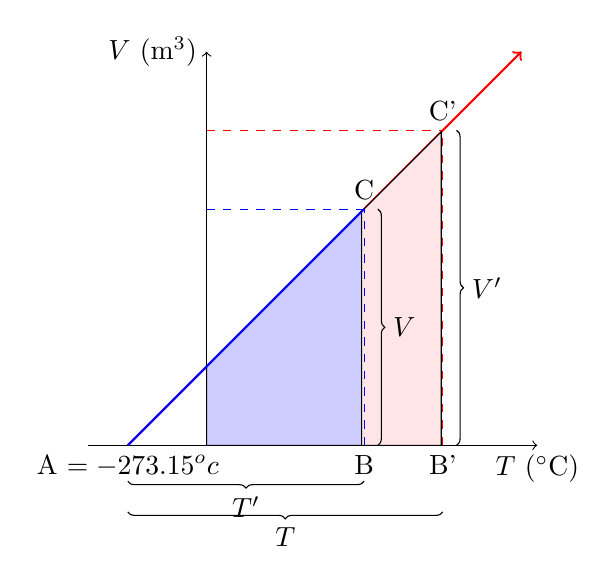
\begin{tikzpicture}
    % axes
    \draw[->] (-1.5,0) -- (4.2,0) node[below] {$T$ ($^\circ$C)};
    \draw[->] (0,0) -- (0,5) node[left] {$V$ (m$^3$)};

    %triangle
    \draw[->,red, thick] (-1,0) -- (4,5);
    \draw[fill=red!10] (0,0) -- (2.98,0) -- (2.98,3.98) -- (0,1) -- cycle;
    \draw[fill=blue!20] (0,0) -- (1.97,0) -- (1.97,2.97) -- (0,1) -- cycle;
    \draw[red, dashed] (3,0) -- (3,4);
    \draw[red, dashed] (0,4) -- (3,4);
    \draw[blue, thick] (-1,0) -- (2,3);
    \draw[blue, dashed] (2,0) -- (2,3);
    \draw[blue, dashed] (0,3) -- (2,3);

    % labels
    \node[anchor = north] at (-1,0) {A $= -273.15^oc$};
    \node[anchor = north] at (2,0) {B};
    \node[anchor = north] at (3,0) {B'};
    \node[anchor = south] at (2,3) {C};
    \node[anchor = south] at (3,4) {C'};

    % length markers for the first triangle
    \draw[decorate,decoration={brace,mirror,raise=5pt}] (-1,-0.28) -- (2,-0.28) node[midway,below=7pt] {$T'$};
    \draw[decorate,decoration={brace,mirror,raise=5pt}] (2,0) -- (2,3) node[midway,right=7pt] {$V$};

    % length markers for the second triangle
    \draw[decorate,decoration={brace,mirror,raise=5pt}] (-1,-0.67) -- (3,-0.67) node[midway,below=7pt] {$T$};
    \draw[decorate,decoration={brace,mirror,raise=5pt}] (3,0) -- (3,4) node[midway,right=7pt] {$V'$};
\end{tikzpicture}

From similiarity of triangle;
\begin{align*}
    \frac{BC}{AB}&=\frac{B'C'}{AB'} \\
    \frac{V}{T}&=\frac{V'}{T'} \\
    \frac{V}{V'}&=\frac{T}{T'}
\end{align*}
for $P$ is Constant

Similiarlly for Pressure at constant Volume

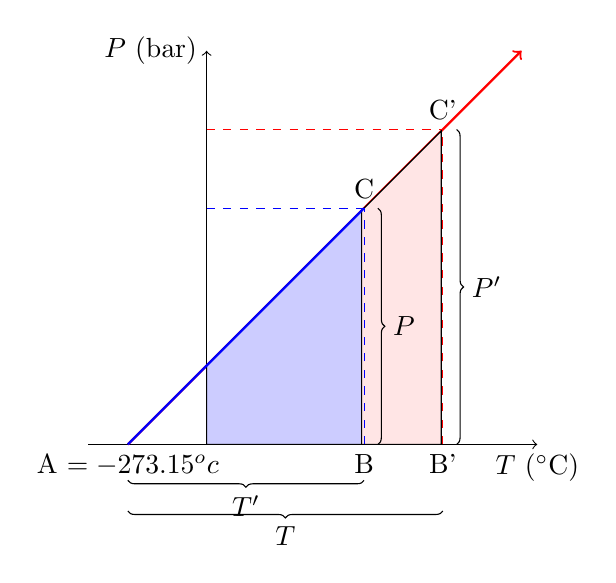
\begin{tikzpicture}
    % axes
    \draw[->] (-1.5,0) -- (4.2,0) node[below] {$T$ ($^\circ$C)};
    \draw[->] (0,0) -- (0,5) node[left] {$P$ (bar)};

    %triangle
    \draw[->,red, thick] (-1,0) -- (4,5);
    \draw[fill=red!10] (0,0) -- (2.98,0) -- (2.98,3.98) -- (0,1) -- cycle;
    \draw[fill=blue!20] (0,0) -- (1.97,0) -- (1.97,2.97) -- (0,1) -- cycle;
    \draw[red, dashed] (3,0) -- (3,4);
    \draw[red, dashed] (0,4) -- (3,4);
    \draw[blue, thick] (-1,0) -- (2,3);
    \draw[blue, dashed] (2,0) -- (2,3);
    \draw[blue, dashed] (0,3) -- (2,3);

    % labels
    \node[anchor = north] at (-1,0) {A $= -273.15^oc$};
    \node[anchor = north] at (2,0) {B};
    \node[anchor = north] at (3,0) {B'};
    \node[anchor = south] at (2,3) {C};
    \node[anchor = south] at (3,4) {C'};

    % length markers for the first triangle
    \draw[decorate,decoration={brace,mirror,raise=5pt}] (-1,-0.28) -- (2,-0.28) node[midway,below=7pt] {$T'$};
    \draw[decorate,decoration={brace,mirror,raise=5pt}] (2,0) -- (2,3) node[midway,right=7pt] {$P$};

    % length markers for the second triangle
    \draw[decorate,decoration={brace,mirror,raise=5pt}] (-1,-0.67) -- (3,-0.67) node[midway,below=7pt] {$T$};
    \draw[decorate,decoration={brace,mirror,raise=5pt}] (3,0) -- (3,4) node[midway,right=7pt] {$P'$};
\end{tikzpicture}

From similiarity of triangle;
\begin{align*}
    \frac{BC}{AB}&=\frac{B'C'}{AB'} \\
    \frac{P}{T}&=\frac{P'}{T'} \\
    \frac{P}{P'}&=\frac{T}{T'}
\end{align*}
for $V$ is Constant

\subsection{Boyle's Law}
Boyle's Law states that, at constant temperature, the pressure of a given amount of gas is inversely proportional to its volume. Mathematically, it is expressed as:
\begin{align}
    P &\propto \frac{1}{V} \\
    PV &= P'V' \\
    PV &= const.
\end{align}
where $P$ is the pressure of the gas, and $V$ is its volume. This implies that if the volume of a gas increases, its pressure decreases, and vice versa, as long as the temperature and the amount of gas remain constant.

\subsection{Avagadro's Law}
Avogadro's Law states that, at the same temperature and pressure, equal volumes of all gases contain the same number of molecules. Mathematically, it is expressed as:
\begin{align}
    V &\propto n
\end{align}
where $V$ is the volume of the gas, and $n$ is the number of moles of the gas. This implies that the volume of a gas is directly proportional to the number of moles, provided temperature and pressure are constant.

For one mole of gas contains $6.023\times10^{23}mol^{-1}$ of particles.

\subsection{Ideal gas Law}
System defined by $(P,V,T)$ undergo change shown in following Fig.\ref{Idealgasprocess}

\begin{figure}[htbp]
    \centering
    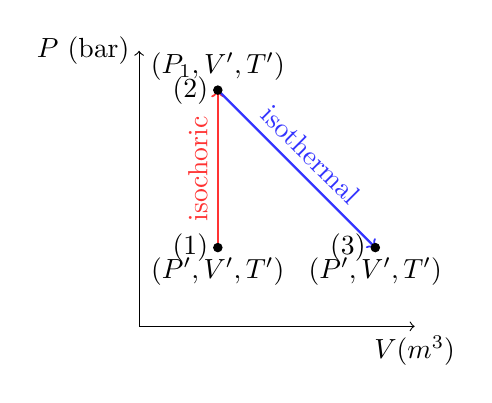
\begin{tikzpicture}
        % axes
        \draw[->] (0,0) -- (3.5,0) node[below] {$V (m^3)$};
        \draw[->] (0,0) -- (0,3.5) node[left] {$P$ (bar)};

        % triangle
        \draw[->,red!80, thick] (1,1) -- (1,3) node[midway,rotate=90,anchor=south] {isochoric};
        \draw[->,blue!80, thick] (1,3) -- (3,1) node[midway,rotate=-45,anchor=south] {isothermal};
        
        \filldraw (1,1) circle (1.5pt) node[anchor=east] {(1)};
        \filldraw (1,3) circle (1.5pt) node[anchor=east] {(2)};
        \filldraw (3,1) circle (1.5pt) node[anchor=east] {(3)};

        % labels
        \node[anchor = north] at (1,1) {$(P',V',T')$};
        \node[anchor = south] at (1,3) {$(P_1,V',T')$};
        \node[anchor = north] at (3,1) {$(P',V',T')$};
    \end{tikzpicture}
    \caption{Diagram illustrating different thermodynamic processes in a $P$-$V$ diagram.}
    \label{Idealgasprocess}
\end{figure}

Apply Gay-Lussac law $(1) \rightarrow (2)$:
\begin{equation} P_1 = P\frac{T'}{T} \label{eq:P'}\end{equation}

Apply Boyle's law $(2) \rightarrow (3)$:
\begin{equation}
\begin{aligned}
    P'V' &= P_1V \\
    &\text{from eq.\ref{eq:P'} we get} \\
    P'V' &= \left(\frac{PT'}{T}\right)V \\
    &\text{after rearranging we get:} \\
    \frac{P'V'}{T'} &= \frac{PV}{T} \\
    \frac{PV}{T} &= \text{const} \\
    PV &=AT \\ 
    &\text{where $A = nR^*$} \\
    &\text{$R^*$ is universal gas constant ($8.314JK^{-1}mol^{-1}$)} \\
    \implies PV&=nR^*T
\end{aligned}
\end{equation}

\subsection{Van Der Waal's equation}
\begin{equation}
    \Big[P+a\Big(\frac{n}{V}\Big)^2\Big]\Big[V-(nb)\Big]=nR^*T
\end{equation}

\noindent Where \\ $a$ = coeff. which characterises the intermolecular forces = $1.35 \times 10^5 Jm^3K^{-1}mol^{-2}$ \\ $b$ = coeff. which accounts for effective volume occupied by molecules = $3.64 \times 10^{-2} m^3 K^{-1}mol^{-1}$ \\
When $nb \rightarrow 0 \text{ or } \frac{n}{V} \rightarrow 0$ Van Der Waal equation $\rightarrow$ Ideal gas equation.

\subsection{Meteorological form of Ideal gas}
Let there be $n$-kilomols particles/molecules of gas.

Therefore the combination of $i^{th}$ component of the gas can be given by:
\begin{equation}
    n=\sum^k_{i=1}n_i
\end{equation}

The total mass of sample in $kg$:
\begin{equation}
    M=\sum^k_{i=1}n_im_i
\end{equation}
where $m_i$ represents molar mass of $i^{th}$ particle/molecule in a sample.\\
Using Ideal gas equation:
\begin{align}
    PV&=nR^*T \\
    \frac{PV}{M} &= \frac{nR^*T}{M} \\    
    P \alpha &= \frac{n}{M} R^* T
\end{align}
since $\frac{V}{M} = \alpha$, and called specfic volume.
\begin{align}
    P \alpha &= \frac{\sum^k_{i=1}n_i}{\sum^k_{i=1}n_im_i} R^* T \\
    P \alpha &= \frac{R^* T}{\bar{m}} \\
    \Rightarrow P \alpha &= R_d T
\end{align}
where $\bar{m}$ is mean molar mass and given by $\frac{\sum^k_{i=1}n_im_i}{\sum^k_{i=1}n_i}$ and $R_d = \frac{R^*}{\bar{m}}$ and unit $JKg^{-1}K^{-1}$ \\

Since we know $\alpha = \frac{1}{\rho}$, where $\rho$ is density of gas. 
\begin{align}
    P \alpha &= R_dT \\
    \Rightarrow P &= \rho R_d T   \label{IdealGasequation}
\end{align}

\begin{question}[label={q:3.2}]{what is $R_d$?}
    $\Rightarrow$ $R_d \rightarrow$ is a specific gas constant where $d$ stands for dry air and this constant is not universal, varies with time and conditons over a particular place.  
    $$R_d = \frac{R^*}{\bar{m}}$$ and unit $JKg^{-1}K^{-1}$
\end{question}

\subsection{Composition of Earth's Atmosphere}

\begin{table}[hbt]
	\centering
	\begin{tabular}{llr}
		\toprule
		Gas & Fraction/Volume & Molecular Mass\\
		\midrule
		$N_2$ & 78.1\% & 28.01 \\
		$O_2$ & 20.9\% & 31.999 \\
		$Ar$ & 0.93\% & 39.9 \\
		\bottomrule
	\end{tabular}
	\label{Composition of Earth Atmosphere}
	\caption{Composition of Earth's Atmosphere.}
\end{table}
We haven't take water vaours($H_2O(v)$), Carbon diaoxide($CO_2$) and Ozone($O_3$) becasue these gaes are highly variable w.r.t time and geography.

\begin{question}[label={q:3.3}]{Find $R_d$ for Earth Atmosphere?}
    \begin{align*}
        \Rightarrow R_d &= \frac{R^*}{\bar{m}} \\
            &= \frac{8.314 \times 10^3}{28.96}\\ 
            &= 0.287085 \\ 
            &= 287.085 Jkg^{-1}K^{-1}
    \end{align*}
\end{question}

% NOTE: COMPLETED L-3
% ------------------------------------------------------------------------------------
\clearpage

\section{Lecture 4 19/08/2024}
$CO_2$ $\rightarrow$ radiation trapping process $\rightarrow$ absorb radiation in IR region of spectrum.

\begin{question}[label={q:4.1}]{
        \begin{enumerate}
            \item Determine the gas constant for the atmosphere of Venus which consists of $95\%$ $CO_2$ and $5\%$ $N_2$ by volume. 
            \item The mean surface temperature of Venus is $740K$ as compared to $288K$ surface temperature of Earth. The surface pressure on Venus is $90$ times that on Eath. By what factor the density of near surafce Venusin atmosphere is greter than the Earth? 
        \end{enumerate}
        }
        $\Rightarrow$ Solution:
        \begin{enumerate}
            \item Mean molar mass of gases of atmosphere of Venus:
                \begin{align*}
                    \bar{m} &= \frac{\sum^k_{i=1} n_im_i}{\sum^k_{i=1}n_i} \\
                    \bar{m} &= 0.95 \times 46 + 0.05\times28 \\
                    \bar{m} &= 43.2
                \end{align*}

                Calculate Specific Molar const.($R_V$) for Venus:
                \begin{align*}
                    R_V &= \frac{R^*}{\bar{m}}  \\
                    \Rightarrow R_V &\approx 192 \text{ $JK^{-1}Kg^{-1}$}
                \end{align*}
            \item Surface Temperature of Venus = $T_V = 740K$  \\
                  Surface Temperature of Earth = $T_V = 740K$  \\
                  Surface Pressure of Earth = $P_E$  \\
                  Surface Pressure of Venus = $P_V = 90 \times P_E$

                  \begin{align*}
                      P_V &= \rho_VR_VT_V \\
                      P_E &= \rho_VR_ET_E
                  \end{align*}
                  \begin{align*}
                      \frac{P_V}{P_E} &= \frac{\rho_V R_VT_V}{\rho_V R_ET_E} \\
                      90 &= \frac{\rho_V}{\rho_E} * \frac{192}{287} * \frac{740}{288} \\
                      \frac{\rho_V}{\rho_E} &= 52.36 
\end{align*}
Venus's atmosphere is $52.36$ times densier than Earth's atmoshpere. \\
$\Rightarrow$ $\rho_E$ = $1.23$ $kgm^{-3}$ and $\rho_V$ = $65.97$ $kgm^{-3}$
        \end{enumerate}
\end{question}

 \begin{question}[label={q:4.2}]{Why $CO_2$ have radiation trapping affinity but not gases like $N_2$?}
    $\Rightarrow$ $CO_2$ has radiation trapping affinity because its molecular structure allows it to absorb and re-emit IR radiation, contributing to the greenhouse effect. This is due to its vibrational modes that change the molecule's dipole moment. In contrast, $N_2$, with its symmetric diatomic structure, cannot absorb infrared radiation effectively, as its vibrations do not change the dipole moment, making it non-contributory to the greenhouse effect.
\end{question}

\subsection{Pressure}
\subsubsection*{Units of Pressure}

Pressure are usually expressed in thefollwing units: \\

1 bar = 1.013 $\times$ 10$^5$ Pa 

10$^5$ Pa = 1000hPa = 1000 mbar

\begin{question}[label={q:4.3}]{Why does ozone layer depletion happen primarily over the South Pole in Antarctica?}
   $\Rightarrow$ Ozone layer depletion happen primarily over the South Pole becasue of following reasons: 
   \begin{itemize}
        \item \textbf{Polar Stratospheric Clouds (PSCs):} During the Antarctic winter, temperatures drop below $-75^\circ$C, leading to the formation of PSCs. These clouds facilitate chemical reactions that convert inactive chlorine compounds into reactive forms, which destroy ozone.

        \item \textbf{Isolation of the Polar Vortex:} The strong polar vortex over Antarctica isolates air, keeping temperatures low and trapping ozone-depleting chemicals within the vortex.

        \item \textbf{Sunlight and Ozone Destruction:} In Antarctic spring, returning sunlight provides energy for reactions between chlorine radicals and ozone, leading to significant ozone depletion and the formation of the "ozone hole."

        \item \textbf{Comparison with the Arctic:} The Arctic has a weaker and less stable polar vortex, resulting in less dramatic ozone depletion compared to Antarctica.
   \end{itemize}
\end{question}

\subsection{Mass of the Atmosphere}

At any point in the atmosphere, atmosphere above will exert a downward force due to gravitational force
\begin{align}
    F &= \rho g \\
    F &= \int^\infty_0 \rho g dz   
\end{align}
 We know $P = \text{Force/(unit area)}$, assuming gravity $g_0$ remain constant, we get:
 \begin{equation}
    \Rightarrow P_s = g_0 \int^\infty_0 pdz
 \end{equation}
 where $P_s$ is vertically integrated and have unit $kgm^{-2}$
 
\begin{question}[label={q:4.4}]{Globally average surface pressure of earth is 985hpa. Estimate mass of atmossphere.}
    $\Rightarrow$ Given $985hpa$ = $985 \times 10^2Pa$ \\
    surface area(sa) = $4\pi r^2$ \\
    where $r$ is radius of earth = $6400km$ \\ 
    we know, pressure($p$) = $\frac{force}{sa}$
    \begin{align*}
        p &= \frac{mg}{4\pi r^2} \\
        986 \times 10^2 &= \frac{m \times 9.81}{4 \times \pi \times (6400 \times 10^3)^2} \\
        m &= 5.168172908\times 10^{18}kg 
    \end{align*}
    $\therefore$ The approximate mass of atmosphere is equal to $5.1708 \times 10^{15}$
\end{question}

\begin{question}[label={q:4.5}]{The average atmospheric pressure on surface of Mars is $6hPa$ and raduis $3400km$. Find mass of Mars.}
    $\Rightarrow$ Given Surface pressure of Mars $P$ = $6hPa = 6 \times 10^2pa$ \\
    Radius of Mars$R$ = $3400km = 3.4 \times 10^6m$\\
    surface area(sa) = $4\pi r^2$ 

    where $r$ is radius of earth. \\ 
    we know, pressure($p$) = $\frac{force}{sa}$
    \begin{align*}
        p &= \frac{mg}{4\pi r^2} \\
        986 \times 10^2 &= \frac{m \times 9.81}{4 \times \pi \times (6400 \times 10^3)^2} \\
        m &= 5.168172908\times 10^{18}kg 
    \end{align*}
    $\therefore$ The approximate mass of atmosphere is equal to $5.168172908\times 10^{18}kg$
\end{question}

% NOTE:COMPLETED L-4
% ------------------------------------------------------------------------------------
\clearpage

\section{Lecture 5 21/08/2024}
In previous lecture, We got equation for Ideal gas Eq.\myeqref{IdealGasequation}, which only deals 
with dry air.

We didn't incooperated moisture!

\begin{center}
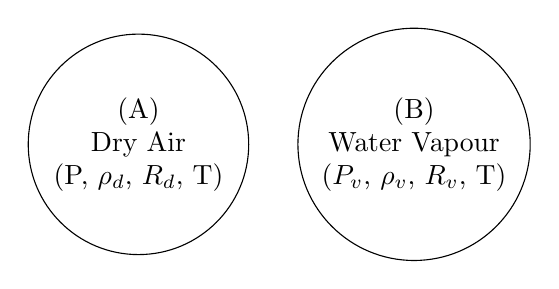
\begin{tikzpicture}
    % Draw the first circle with text confined inside
    \node[draw, circle, minimum size=2.8cm, align=center] at (0, 0) {(A) \\ Dry Air \\ (P, $\rho_d$, $R_d$, T)};

    % Draw the second circle with text confined inside
    \node[draw, circle, minimum size=2.8cm, align=center] at (3.5, 0) {(B) \\ Water Vapour \\ ($P_v$, $\rho_v$, $R_v$, T)};
\end{tikzpicture}
\end{center}

where $P_v$ is vapour pressure and given by 
\begin{align}
    P_v &= \rho_v R_v T \label{vapourpressure} \\
    R_v &= \frac{R^*}{\bar{m}} = \frac{8.314 \times 10^3}{18.01} = 461.63 JK^{-1}kg^{-1} 
\end{align}

\textbf{Note:} Water vapour is not same as moisture, misture is mixture of air and water vapour

\subsection{Dalton's law of partial pressure}
Dalton's law of partial pressure states that total pressure exerted by the mixture of gas is equal to the sum of partial pressure exerted by individual contituent at a given temperature.   
\begin{equation}
    P = P_d + e  \label{eq:Totalpartialpressure}
\end{equation}
Where
\begin{align*}
    P &= \text{ Total pressure excerted by all gases in mixture}\\
    P_d &= \text{Pressure exerted by dry air} \\
    e &= P_v = \text{Vapour pressure}
\end{align*}
Substituting Eq.\myeqref{IdealGasequation} and Eq.\myeqref{vapourpressure} in Eq.\myeqref{eq:Totalpartialpressure}, we get:
\begin{align}
    P = \rho_d R_d T + \rho_v R_v T \\
    P = (\rho_d R_d + \rho_v R_v) T
\end{align}

\subsection{Humidity}
We define humidity using following parameters:
\begin{enumerate}
    \item Mixing ratio:
        \begin{align}
            \omega &= \frac{ \text{Mass of water vapour}}{\text{Mass of dry air}} = \frac{M_v}{M_d} \\
                   &=\frac{ \text{Densityof water vapour}}{\text{Density of dry air}}= \frac{\rho_v}{\rho_d}
            \label{eq:mixingratio}
        \end{align}
        \text{Unit of mixing ratio is $g/Kg$}
    \item Specific heat:
        \begin{align}
            q &= \frac{ \text{Mass of water vapour}}{\text{Mass of dry air} + \text{Mass of water vapour}} \\
              &= \frac{M_v}{M_d} \\
              &= \frac{ \text{Density of water vapour}}{\text{Density of dry air} + \text{Density of water vapour}} \\
              &= \frac{\rho_v}{\rho_d+\rho_v} \\
              &= \frac{\rho_v}{\rho}
            \label{Specificheat}
        \end{align}
        \text{w $\approx$ q, $\because$ mass of water vapour $\ll$ masss of dry air}
        \begin{align}
            \omega &= \frac{\rho_v}{\rho_d} \\
                &= \frac{e/R_v T}{P_d/R_d T} \\
                &= \frac{e\epsilon}{P_d} \\ 
                &= \frac{e\epsilon}{P-e} \\
                &\approx \frac{e\epsilon}{P}
        \end{align}
        \text{where $\epsilon = \frac{R_d}{R_v}$ = 0.621} \\
    \text{Similiary,}
    \begin{align*}
        q &= \frac{\rho_v}{\rho_v + \rho_d} \\
          &= \frac{e\epsilon}{P-(1-\epsilon)e} \\
          &\approx \frac{e\epsilon}{P} \\ 
        q &\approx w   
    \end{align*}
\end{enumerate}

\subsection{Ideal gas equation for moist gas}
Total pressure 
\begin{align*}
    P &= P_d + e \\
     &= \rho_d R_d T + \rho_v R_v T \\
     &= \rho_d R_d T \left[ 1 + \frac{\rho_v R_v}{\rho_d R_d} \right] \\
     &= \rho_d R_d T \left[ 1 + \frac{\rho_v}{\rho_d}\cdot \frac{R_v}{R_d} \right] \\
     &= \rho_d R_d T \left[ 1 + \frac{\rho_v}{\rho_d}\cdot \frac{1}{\epsilon} \right] \\
     &= \rho_d R_d T \left[ 1 - \left(1 - \frac{1}{\epsilon}\right) \frac{\rho_v}{\rho} \right]
\end{align*}

\begin{align}
   \therefore P  &= \rho_d R_d T \left[ 1 - \left(1 - \frac{1}{\epsilon}\right)\cdot q \right] \label{eq:Preessureofmosistgas}
\end{align}

\textbf{Virtual Temerature}
% FIX:Virtual temperature is defined as temperature of dry gas parcel which would have to have inorder to that the parcel's density is equal to density of moist parcel, assuming pressure
\begin{align}
    \Rightarrow T_v &= \frac{P}{\rho_d R_d} = T\left[ 1 - \left(1 - \frac{1}{\epsilon}\right)\cdot q \right] \label{eq:virtualtemp}
\end{align}

Therefore from Eq.\myeqref{eq:Preessureofmosistgas} and Eq.\myeqref{eq:virtualtemp}, we get:
\begin{equation}
    P = \rho_d R_d T_v
    \label{eq:pressureintermsofT_v}
\end{equation}

\begin{center}
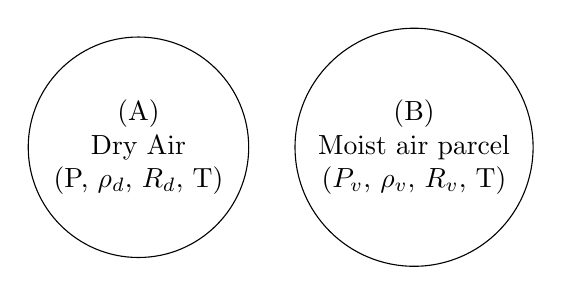
\begin{tikzpicture}
    \node[draw, circle, minimum size=2.8cm, align=center] at (0, 0) {(A) \\ Dry Air \\ (P, $\rho_d$, $R_d$, T)};
    \node[draw, circle, minimum size=2.8cm, align=center] at (3.5, 0) {(B) \\Moist air parcel\\ ($P_v$, $\rho_v$, $R_v$, T)};
\end{tikzpicture}
\end{center}

$\rho_d > \rho_m$ $\xrightarrow{\triangle}$ $\rho_d = \rho_m$, where $\triangle$ represents heat. \\

\begin{question}[label=q:5.1]{On a summer day\, the AC breaks down and the air in the classroom becomes warm and muggy with a vapour pressure of $20 \text{ hPa}$ and a temperature of $25^\circ\text{C}$. \newline
        a. \text{If the volume of the classroom is $40 \text{m}^3.$ How } \text{much water is present in the room in vapour form?}
        b. \text{If pressure of the room is $900 hPa$ then what is} \text{virtual temerpature of the air?}
}
$\Rightarrow$ a. We have, 
        \begin{align*}
            P_v &=\rho_v R_v T \\
            20 \times 10^2 &= \rho_v \times 461.62 \times 298 \\
            \rho_v &= 0.0145 \, kg/m^3 \\
            \frac{m}{V} &= 0.0145 \\
            \frac{m}{40} &= 0.0145 \\
            m &\approx 0.58149 \, kg
        \end{align*}
        $\therefore$ Amount of water vapour in room is $0.58148976 \,  kg$. \\

$\Rightarrow$ b. Given, $P = 900 \, \text{hPa} = 90000 \, \text{Pa} $ \\
        Let $T_v$ be the virtual temperature. We know:
        \begin{align*}
            T_v = T \left(1 + 0.61 \frac{P_v}{P} \right)
        \end{align*}
        Substituting the values:
        \begin{align*}
            T_v &= 298 \left(1 + 0.61 \times \frac{2000}{90000} \right)  \\
            T_v &= 298 \times 1.01356 \\
            T_v &\approx 302.04 \, \text{K}
        \end{align*}
        $\therefore$ The virtual temperature of the air is approximately $ 302.04 \, \text{K} $.
\end{question}

% NOTE: COMPLETED L-5
% ------------------------------------------------------------------------------------
\clearpage

\section{Lecture 6 28/08/2024}

\subsection{Archimedes Principle}
Archimedes' principle states that any object completely or partially submerged in a fluid (liquid or gas) is buoyed up by a force equal to the weight of the fluid that the object displaces.

\begin{quote}
\raggedright
\textbf{Upward force exerted by the fluid = weight of the fluid displaced by the object}
\end{quote}

\subsection{Buoyancy}
Buoyancy is the upward force exerted by a fluid (liquid or gas) that opposes the weight of an object submerged in it.

\begin{center}
    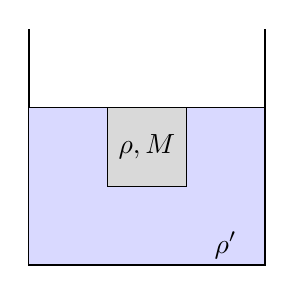
\begin{tikzpicture}
        % Draw the container using three solid lines
        \draw[thick] (0,0) -- (0,3); % left line of the container
        \draw[thick] (3,0) -- (3,3); % right line of the container
        \draw[thick] (0,0) -- (3,0); % bottom line of the container

        % Draw the fluid level using a dashed line
        % \draw[dashed] (0,1.5) -- (3,1.5); % dashed line representing fluid level
        % \draw[dashed] (0,1) -- (3,1); % dashed line representing fluid level
        % \draw[dashed] (0,0.5) -- (3,0.5); % dashed line representing fluid level
        \draw[fill=blue!15] (0,0) rectangle (3,2); % square representing the object

        % Draw the floating object (square) on the fluid surface
        \draw[fill=gray!30] (1,1) rectangle (2,2); % square representing the object

        % Labels for densities
        \node at (2.5,0.25) {\(\rho'\)}; % label for fluid density
        \node at (1.5,1.5) {\(\rho , M\)}; % label for object density
    \end{tikzpicture}
\end{center}

Net force acting on mass($M$) and density($\rho$) submerged in fluid of density($\rho'$) is given by:
\begin{align}
    F_B &= \rho' Vg - Mg  \label{eq:buoyancy_force} \\
        &= \rho' Vg - \rho Vg \\
        &= (\rho' - \rho) Vg
\end{align}
Dividing equation with $M$ on both side,
\begin{align}
    \frac{F_B}{M} &= \frac{(\rho' - \rho) Vg}{M} \\
    f_B              &= \frac{(\rho' - \rho) Vg}{\rho V} \\
                     &= \Big(\frac{\rho'}{\rho}-1\Big)g  \label{eq:acceration_due_to_buoyancy}
\end{align}

If Buoyant force per unit mass ($f_B$),
\begin{align*}
    f_B > 0 &\rightarrow \text{upward force} \\ 
        f_B < 0 &\rightarrow \text{downward force}
\end{align*}

We don't measure density in real case scenario, so we need to convert the equation in the useful form.

Assume pressure inside air parcel and surrounding equal and process to be reversible.

Using Ideal gas equation,
\begin{align}
    P &= \rho R_d T_v \label{eq:Pressure_of_mass}\\
    P &= \rho' R_d T_v' \label{eq:Pressure_of_fluid}
\end{align}

Substituting equation Eq.\myeqref{eq:Pressure_of_mass} \& \myeqref{eq:Pressure_of_fluid} in Eq.\myeqref{eq:acceration_due_to_buoyancy}, we get:
\begin{align}
    f_B &= \frac{\big(\frac{P}{R_d T_v'} - \frac{P}{R_d T_v}\big)}{\frac{P}{R_d T_v'}}g \\
    \Rightarrow f_B &= \frac{(T_v - T_v')}{T_v'}g
\end{align}
where $T_v$ and $T_v'$ are virtual temperture of of parcel and fluid respectively. 
\begin{align*}
    f_B > 0 \rightarrow T_v &> T_v' \rightarrow \text{upward force} \\ 
    f_B < 0 \rightarrow T_v &< T_v' \rightarrow \text{downward force} \\
    f_B = 0 \rightarrow T_v &= T_v' \rightarrow \text{no net force}
\end{align*}

\begin{question}[label=q:6.1]{A parcel ofair has a temperature of $29^\circ C$ and specific humidity of $24 g/kg$. It is embedded in the environment having termperature of $30^\circ C$ and specific humidity of $5g/kg$ \newline
        a. \text{What is vertical acceleration?} \\
        b. \text{If there are no forces acting on in, how long }\\ \text{would take for thep parcel to raise $10m$ from} \\ \text{starting position?}
    }
    $\Rightarrow$ a. Given $T_{v,a} =29^\circ C= 302K$ and $T_{v,s} =30^\circ C= 303K$,\\ 
                    $q_a=R.H._a = 24g/kg$, \\
                    $q_s=R.H._s = 5g/kg$,\\ 
        We know, 
        \begin{align*}
            T_{v,a} &= T_a(1+0.61q_a)\\
                    &= 302(1+0.61 \times 24 \times 10^{-3}) \\
                    &= 306.42128 K \\
            T_{v,s} &= T_s(1+0.61q_s)\\
                    &= 303(1+0.61 \times 5 \times 10^{-3}) \\
                    &= 303.92415 K
        \end{align*}
        Buoyant force per unit mass $f_B$,
        \begin{align*}
            f_B &= \Big(\frac{T_{v,a} - T_{v,s}}{T_{v,s}}\Big)g\\
                &= \Big(\frac{306.42128 - 303.92415}{303.92415}\Big)\times 9.81\\
                &= 0.0806 m/s^2
        \end{align*}
    \text{$\therefore$ Vertical accerleration due to buoyant force is} \\ \text{$0.0806 m/s^2$.} \\

    $\Rightarrow$ b. Given Height $h=10m$, \\
                           Vertical accerlation $a=f_B=0.0806 m/s^2$ \\

        Using equation of motion:
        \begin{align*}
            s &= \frac{1}{2} at^2 \\
            10 &= \frac{1}{2} \times 0.0806 \times t^2 \\
            t &= 15.7524 s
        \end{align*}
    \text{$\therefore$ Time taken by parcel to rasie $10m$ due to buoyant} \\ \text{force is $15.75$ seconds.} \\
\end{question}

\subsection{Hydrostatic equation}

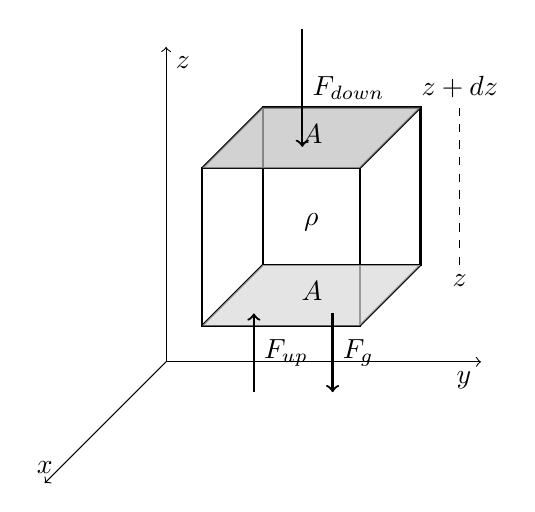
\begin{tikzpicture}[scale=1]
    % Draw the coordinate axes
    \draw[->] (0,0,0) -- (0,0,4) node[anchor=south]{$x$};
    \draw[->] (0,0,0) -- (4,0,0) node[anchor=north east]{$y$};
    \draw[->] (0,0,0) -- (0,4,0) node[anchor=north west]{$z$};

    % Draw cube
    \draw[thick] (2,2,2) -- (4,2,2) -- (4,4,2) -- (2,4,2) -- cycle; % Bottom face
    \draw[thick] (2,2,4) -- (4,2,4) -- (4,4,4) -- (2,4,4) -- cycle; % Top face
    \draw[thick] (2,2,2) -- (2,2,4); % Vertical edges
    \draw[thick] (4,2,2) -- (4,2,4);
    \draw[thick] (4,4,2) -- (4,4,4);
    \draw[thick] (2,4,2) -- (2,4,4);

    % Add nodes for z and z+dz
    \node at (4.5,2,2) [below] {$z$}; % Node at the start of the line
    \node at (4.5,4,2) [above] {$z+dz$}; % Node at the end of the line

    % Draw height range from z to z+dz
    \draw[dashed] (4.5,2,2) -- (4.5,4,2); % Dashed line from z to z+dz

    % Shade the upper and lower faces
    \fill[gray!30,opacity=0.7] (2,2,4) -- (4,2,4) -- (4,2,2) -- (2,2,2) -- cycle; % Bottom face
    \fill[gray!50,opacity=0.7] (2,4,4) -- (4,4,4) -- (4,4,2) -- (2,4,2) -- cycle; % Top face

    \node at (3,2.7,3) [above] {$\rho$}; % Node at the end of the line
    \node at (3.2,4,3.5) [above] {$A$}; % Node at the end of the line
    \node at (3.2,2,3.5) [above] {$A$}; % Node at the end of the line

    % Add force arrows on the faces
    \draw[->, thick] (2.5,5,2) -- (2.5,3.5,2) node[midway, right] {$F_{down}$}; % Force on top face
    \draw[->, thick] (1.5,0,1) -- (1.5,1,1) node[midway, right] {$F_{up}$}; % Force on top face
    \draw[->, thick] (2.5,1,1) -- (2.5,0,1) node[midway, right] {$F_{g}$}; % Force on top face
\end{tikzpicture}

\begin{enumerate}
    \item The downward force due to gravity:
          \begin{equation}
              F_g = mg = \rho(A\delta z)g
          \end{equation}
    \item The upward force due to atmosphere force acting on the bottom of the slab is given by:
        \begin{equation}
        F_{up} = Ap(z)
        \end{equation}
    \item The downward force acting on parcel:
        \begin{equation}
        F_{down} = Ap(z+dz)
        \end{equation}
\end{enumerate}
$\therefore$ Net upward fore will be given by Eq.\myeqref{eq:Net_upward_force}
\begin{align}
    F &= F_{up} - F_{down} - F_g \\
     &= Ap(z) - Ap(z+dz) - \rho(A\delta z)g \label{eq:Net_upward_force}
\end{align}

Hence, Upward acccleration will be:
\begin{align}
    a &= \frac{F}{\rho A \delta z} \\
      &= \frac{Ap(z) - Ap(z+ \delta z) - (A\delta z)\rho g}{\rho A \delta z} \\
      &= -\frac{1}{\rho} \Big[\frac{p(z+ \delta z) - p(z)}{\delta z} \Big] - g
    \label{eq:upward_acc}
\end{align}
Taking $\lim_{\delta z \to 0}$
\begin{align}
    \Rightarrow a+g = -\frac{1}{\rho} \frac{dp}{dz}
    \label{eq:hydrostatic_eq}
\end{align}
Eq.\myeqref{eq:hydrostatic_eq} is called Hydrostatic equation.

\begin{question}[label=q:6.2]{Velocity of hyricene is $10m/s$ and time taken $10 min$ find acceleration.}
 $\Rightarrow$ Acceleration $a= \frac{v}{t} = \frac{10}{10\times 60} = \frac{10}{600} \approx 0.0167$
\end{question}

From the above example question \ref{q:6.2} we can infer that $a + g \approx g$, 

$\therefore$ we can rewrite Hydrostatic equation as following Eq.\myeqref{eq:hydrostatical_approximation}: 
\begin{equation}
    \Rightarrow g = -\frac{1}{\rho} \frac{dP}{dz}
    \label{eq:hydrostatical_approximation}
\end{equation}
This is called \textbf{Hydrostatication approximation}.

% NOTE: COMPLETED L-6
% --------------------------------------------------------------------------------------
\clearpage

\section{Lecture 7 29/08/2024}
\subsection{Ideal gas equation with Hydostatic equation}
From Ideal gas equation:
\begin{align}
    P &= \rho R_d T_v \\
    \rho &= \frac{P}{R_d T_v} 
\end{align}
Substitute $\rho$ in hydrostactic Eq.\myeqref{eq:hydrostatical_approximation}, we get:
\begin{align}
    g &= - \frac{R_dT_v}{P}\frac{\partial P}{\partial z}\\
    \frac{\partial P}{\partial z} &= -\frac{P}{R_d T_v}g \\
    \frac{1}{P} \frac{\partial P}{\partial z} &= -\frac{g}{R_d T_v} \\
    \frac{\partial \ln P}{\partial z} &= -\frac{g}{R_d T_v}    
\end{align}
The rate of change of logarithm of pressure is Inversely proportional to temperature and does not depend on pressure.

\subsection{Geopotential}
Geopotential at any point in the atmosohere is defined as the work done against the gravitational field to raise a mass of $1kg$ from sea level to that point,

Represnted by Eq.\myeqref{eq:geopotential} and has unit $Jkg^{-1}$
\begin{equation}
    d\phi = gdz
    \label{eq:geopotential}
\end{equation}

From hydrostatic equation Eq.\myeqref{eq:hydrostatic_eq},
\begin{align}
     dp &= -\rho g dz \\
     gdz &= -\frac{1}{\rho} dp \\
     gdz &= -\alpha dp
\end{align}
where $\alpha$ is specific volume.

Intergrating Eq.\myeqref{eq:geopotential}, we get:
\begin{align}
    \int^{\phi(z)}_{0} d\phi &= \int^{z}_{0} gdz \\
    \phi(z) &= \int^{z}_{0} gdz
\end{align}

Let $g_0$ be accerleration due to gravity averaged over the surface.
\begin{align}
    \frac{\phi(z)}{g_0} &= \int^{z}_{0} \frac{g}{g_0}dz \\
    \Rightarrow Z &= \frac{\phi(z)}{g_0} \label{eq:geopotential_height}
\end{align}
The \textbf{$Z$ in Eq\myeqref{eq:geopotential_height} is called Geopotential height}.

\begin{table}[ht]
\centering
\begin{tabular}{|>{\centering\arraybackslash}m{2cm}|>{\centering\arraybackslash}m{2cm}|>{\centering\arraybackslash}m{1.5cm}|}
\hline
\textbf{z (km)} & \textbf{Z (km)} & \textbf{g (m/s\textsuperscript{2})} \\ \hline
0   & 0     & 9.81 \\ \hline
1   & 1     & 9.80 \\ \hline
10  & 9.99  & 9.77 \\ \hline
100 & 98.87 & 9.50 \\ \hline
500 & 46.36 & 8.43 \\ \hline
\end{tabular}
\caption{Deviation of vaules of $g$ for Geometric Height($z$), Geopotential Height($Z$)}
\end{table}

\begin{align}
    p &= \rho R_d T_v \\
    p \alpha &= R_d T_v \\
    \alpha &= \frac{R_d T_v}{p}
\end{align}
\begin{align}
    d\phi &= gdz = -\alpha dp \\
    d\phi &= -\frac{R_d T_v}{p}dp
\end{align}
Integrating from both sides, we get:
\begin{align}
    \int^{\phi_2}_{\phi_1}d\phi &= \int^{P_2}_{P_1}-\frac{R_d T_v}{p}dp \\
    \phi_2-\phi_1 &= -R_d \int^{P_2}_{P_1}T_v\frac{dp}{p}
\end{align}
Dividing both side with $g_0$, we get:
\begin{align}
    \frac{(\phi_2-\phi_1)}{g_0} &= -\frac{R_d}{g_0}\int^{P_2}_{P_1}T_v\frac{dp}{p} \\
    (Z_2-Z_1) &= -\frac{R_d}{g_0}\int^{P_2}_{P_1}T_v\frac{dp}{p}
\end{align}
By assuming isothermal atmosphere
\begin{align}
    (Z_2-Z_1) &= -\frac{R_d}{g_0}\int^{P_2}_{P_1}\bar{T}_v\frac{dp}{p} \\
    (Z_2-Z_1) &= -\frac{R_d}{g_0}\bar{T}_v\ln\Big(\frac{dp}{p}\Big) \\
    \Rightarrow (Z_2-Z_1) &= -H\ln\Big(\frac{dp}{p}\Big) \label{eq:hypsometric_eq}
\end{align}
Where $\bar{T}_v$ is average temperature of atmosphere taken over geopotnetial ($\phi_1 \& \phi_2$) and $H$ is scale height giev by Eq.\myeqref{eq:scale_height}:
\begin{equation}
    H = \frac{R_d T_v}{g_0}
    \label{eq:scale_height}
\end{equation}

\textbf{Scale height $H$} is defined as height at which the pressure reduces to $1/e$ times the surface pressure. It is around $7.8km$ for Earth's atmosphere.

Eq.\myeqref{eq:hypsometric_eq} is called Hypsometric equation. \\
Simplifing Eq.\myeqref{eq:hypsometric_eq}, we get:
\begin{align}
    P_2 &= P_1 e^{-\frac{(Z_2-Z_1)}{H}} \\
    \Rightarrow P &= P_0 e^{-\frac{(Z_2-Z_1)}{H}}
\end{align}

\begin{question}[label={q:7.1}]{}
    $\Rightarrow$ Solution, \begin{align*}
        (Z_2-Z_1) &= -\frac{R_d}{g_0}\bar{T}_v\ln\Big(\frac{dp}{p}\Big) \\
                  &= -\frac{287 \times 255}{9.81} \ln{\frac{P_2}{P_1}} \\
                  &= -7.4\ln{\frac{P_2}{P_1}}
    \end{align*}
\end{question}

% NOTE: COMPLETED L-7
% --------------------------------------------------------------------------------------
\clearpage

\section{Lecture 8 30/08/2024}
\begin{question}[label=q:8.1]{On May 20\,2020  tropical cyclone Ampan of cetre pressure at ocean surface dropped to $920hPa$. The surrounding region away from influence of centre of cyclone had mean sea level pressure of $1010hPa$. The height depression associtated with centre of cyclone vanished at height of pressure level of $150hPa$. If the mean virtual temperature of the surrounding between the surface at $150hPa$ was $-10^{\circ}C$. What was the corresponding mean virtual temperature in the centre of storm?}
    $\Rightarrow$ Given data:
    \begin{align*}
         P_1 &= 1010 hPa = 101000 Pa \\
         P_2 &= 920 hPa = 92000 Pa \\
         P_3 &= 150 hPa = 15000 Pa \\
         T_{v,surr} &= -10^\circ C = 263.15 K \\
         R_d &= 287 J/(kg K) \\
         g_0 &= 9.81 m/s^2
    \end{align*}

    $\Rightarrow$ Height difference calculation in the surrounding air:
    \begin{align*}
        (Z_2 - Z_1) &= \frac{R_d T_{v,\text{surr}}}{g_0} \ln\left(\frac{P_1}{P_3}\right) \\
        &= \frac{287 \times 263.15}{9.81} \ln\left(\frac{101000}{15000}\right) \\
        &= 7701.43 \times 1.906 \\
        &= 14681.92 \, \text{m}
    \end{align*}

    $\Rightarrow$ Solution for mean virtual temperature at the center of the storm:
    \begin{align*}
        (Z_2 - Z_1) &= -\frac{R_d}{g_0} \bar{T}_{v,\text{center}} \ln\left(\frac{P_3}{P_2}\right) \\
        14681.92 &= -\frac{287}{9.81} \bar{T}_{v,\text{center}} \ln\left(\frac{15000}{92000}\right) \\
        \bar{T}_{v,\text{center}} &= -\frac{14681.92 \times 9.81}{287 \ln\left(\frac{15000}{92000}\right)} \\
        &= -\frac{14681.92 \times 9.81}{287 \times (-1.7749)} \\
        &= \frac{144040.6}{-509.4613} \\
        &= 282.72 \, \text{K} \\
        T_{v,\text{center}} &\approx 282.72 - 273.15 \\
        T_{v,\text{center}} &\approx 9.57^\circ \text{C}
    \end{align*}
\end{question}

\begin{question}[label=q:8.2]{Calculate the thickness of layer between $1000hPa$ and $500hPa$ pressure surface.\newline
    a. At point in tropics where $T_v$ is $15^{\circ}C$ \\
    b. At point in polar where $T_v$ is $-40^{\circ}C$ 
}
Solution
 $\Rightarrow$  a. \begin{align*}
    (Z_2-Z_1) &= -\frac{R_d}{g_0}\bar{T}_v\ln\Big(\frac{dp}{p}\Big) \\
              &= \frac{287\times 288 K}{9.81 m/s^2} \ln\frac{1000 hPa}{500 hPa} \\
              &= 5840.2419km
    \end{align*}
 $\Rightarrow$  b. \begin{align*}
    (Z_2-Z_1) &= -\frac{R_d}{g_0}\bar{T}_v\ln\Big(\frac{dp}{p}\Big) \\
              &= \frac{287\times 233 K}{9.81 m/s^2} \ln\frac{1000 hPa}{500 hPa} \\
              &= 4724.9179km
    \end{align*}
\end{question}

\subsection*{Pressure profiles in the idealized atmosphere}
\addcontentsline{toc}{subsection}{Pressure profiles in the idealized atmosphere} % Adds this subsection to the table of contents

\subsection{Constant density atmosphere}
Assume atmosphere is at hydrostatic balance and density $\rho$ to be constant.
\begin{align}
    dP &= -\rho gdz \\ 
    \int^{P(z)}_{P(0)} dP &= -\int^{z}_{0} \rho g dz \\
    p(z)-p(0) &= -\rho gz
\end{align}
Substituting values in above eqaution, we obtain: 
\begin{align}
    (0 - 101.3) &= -1.23 \times 9.8 \times z \\
    z &\approx 8.3952 km
\end{align}

Using Ideal gas equation, substitute $P$,
\begin{align}
    d(\rho RT) &= -\rho gdz \\ 
    RdT &= -gdz \\ 
    dT &= -\frac{g}{R}dz \\ 
    T(z) - T(0) &= \frac{g}{R}(z-0) \\
    T(z) &= T(0) - \frac{g}{R}z \\
    T(z) &= T(0) - 0.0341z
\end{align}
\begin{align}
    T(z) &= T(0) - 34.1z
\end{align}
where $34.1$ constant have an unit of $^\circ C/km$
\begin{align}
    \Rightarrow \Gamma &= -\frac{dT}{dz} = -\frac{g}{R} = -34.1^\circ C/km 
\end{align}
This is Ideal/theoritical value, but \textbf{actual/pratical value for $Gamma$ is $6.5^\circ/km$} because of phenomenon called \textbf{auto-convetive lapse rate} i.e. $\rho$ varies with altitude, and warm are and cold air do vertical circulation.

\subsection{Constant temperature atmosphere}
Assume atmosphere is at hydrostatic balance and Temperature $T$ to be constant.
\begin{align}
    dP &= -\rho gdz \\ 
    d \rho R T &= -\rho g dz \\
    p(z)-p(0) &= -\rho gdz \\
    RTd\rho &= -\rho gdz \\
    \frac{d\rho}{\rho} &= -\frac{g}{RT}dz \\
    \ln{\rho} |^{\rho_2}_{\rho_1} &= -\frac{g}{RT}z |^{z}_{0} \\
    \Rightarrow \ln{\frac{\rho_2}{\rho_1}} &= -\frac{g}{RT}z
\end{align}

\subsection{Constant lapse rate atmosphere}
\begin{align}
    T &= T_0-\Gamma_z \\
    dP &= -\rho gdz \\ 
    \frac{dP}{dz} &= -\frac{Pg}{R T} \\ 
    \frac{dP}{dz} &= -\frac{Pg}{R (T_0-\Gamma_z)} \\ 
    \frac{1}{P}dP &= -\frac{gdz}{R (T_0-\Gamma_z)}\\ 
    \int_{P_1}^{P_2}\frac{1}{P}dP &= -\frac{g}{R} \int^z_0 \frac{dz}{(T_0-\Gamma_z)}\\ 
    \Rightarrow \ln{\frac{P_2}{P_1}} &= -\frac{g}{R\Gamma_z} \ln{\Big(\frac{T_0-\Gamma_z}{T_0}\Big)}
\end{align}

% NOTE: COMPLETED L-8
% -------------------------------------------------------------------------------------
\clearpage

\section{Lecture 9 04/09/2024}
\subsection{1$^{st}$ law of thermodynamics and it's application}
\subsubsection*{Pressure-volume work}
Work done $\delta w$ by any force $F$ to displace object with diplacement $ds$ is equal to:
\begin{equation}
    \delta w = F \cdot ds
    \label{eq:work_done}
\end{equation}

Incremental Work done by Force $F$ to increase the volume will be given as follows:
\begin{align}
    \delta w &= F \cdot ds \\
    &= PA\cdot ds \\
    &= PdV
    \label{eq:Pressure_volume_work}
\end{align}
Assuming Pressure $P$ constant at each step, and process is slow, incremental, i.e, reversible.


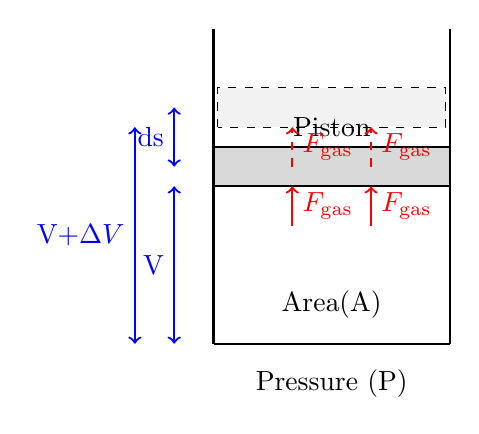
\begin{tikzpicture}
    % Piston cylinder outline (topless)
    %\draw[thick] (0, 0) rectangle (3, 5.5); % Cylinder with open top
    \draw[thick] (0, 0) -- (3, 0);  % Closed bottom
    \draw[thick] (0, 0) -- (0, 4);  % Left wall
    \draw[thick] (3, 0) -- (3, 4);  % Right wall
    

    % Piston 1 (dashed and offset slightly to the back)
    \draw[dashed, fill=gray!10] (0.05, 2.75) rectangle (2.95, 3.25); % Offset slightly to show both dashed and thick lines
    % Piston 2 (thick, inside the cylinder)
    \draw[thick, fill=gray!30] (0, 2) rectangle (3, 2.5); % Piston inside the cylinder

    % Arrows showing motion of piston
    \draw[<->, blue, thick] (-0.5, 2.25) -- (-0.5, 3) node[midway, left] {ds};
    
    % Labels for points
    \node at (1.5, 0.5) {Area(A)}; % Point A above the piston
    \node at (1.5, 2.75) {Piston}; % Label for piston

    % Annotate pressure and volume
    \draw[<->, blue, thick] (-0.5, 0) -- (-0.5, 2) node[midway, left] {V};
    \draw[<->, blue,thick] (-1, 0) -- (-1, 2.75) node[midway, left] {V+$\Delta V$};
    \node at (1.5, -0.5) {Pressure (P)};

    % Force arrows on piston
    \draw[->, red, thick] (1, 1.5) -- (1, 2) node[midway, right] {$F_{\text{gas}}$}; % External force (downward)
    \draw[->, red, thick] (2, 1.5) -- (2, 2) node[midway, right] {$F_{\text{gas}}$}; % External force (downward)

    \draw[->, dashed, red, thick] (1, 2.25) -- (1, 2.75) node[midway, right] {$F_{\text{gas}}$}; % External force (downward)
    \draw[->, dashed, red, thick] (2, 2.25) -- (2, 2.75) node[midway, right] {$F_{\text{gas}}$}; % External force (downward)
    
\end{tikzpicture}

\begin{tikzpicture}

    % Axes
    \draw[->] (0,0) -- (6,0) node[below] {Volume (V)};
    \draw[->] (0,0) -- (0,5) node[left] {Pressure (P)};
    
    % Piston curve (work process)
    \draw[thick,domain=1:5,samples=100,smooth,variable=\x] plot (\x, {5/\x}) node[right] {};
    
    % Marking points A and ds on the curve
    \filldraw[blue] (2.5,2) circle (2pt) node[above right] {A};
    \filldraw[red] (4,1.25) circle (2pt) node[above right] {ds};
    
    % Labeling the curve
    \node at (3,3) {$P(V)$};
    
    % Dashed lines for A and ds
    \draw[dashed] (2.5,0) -- (2.5,2);
    \draw[dashed] (0,2) -- (2.5,2);
    
    \draw[dashed] (4,0) -- (4,1.25);
    \draw[dashed] (0,1.25) -- (4,1.25);

    % Labeling the work done
    \node at (5,4) {Work done: $\int PdV$};

\end{tikzpicture}
% NOTE: COMPLETED L-9
% --------------------------------------------------------------------------------------
\clearpage

\section{Lecture 10 05/09/2024}
\subsection{. 1$^{st}$ law of thermodynamics and it's application}

\begin{equation}
    \Delta U = Q-W
    \label{eq:1st_law}
\end{equation}

\subsubsection*{Mechanical work}
\begin{equation}
    \delta w = F \cdot ds
    \label{eq:mechanical work}
\end{equation}

\subsubsection*{Pressure-volume work}
\begin{align}
    \delta w &= PA\cdot ds \\
    \delta w &= PdV \\
    w &= \int_i^f PdV
    \label{eq:Pressure_volume_work_done}
\end{align}

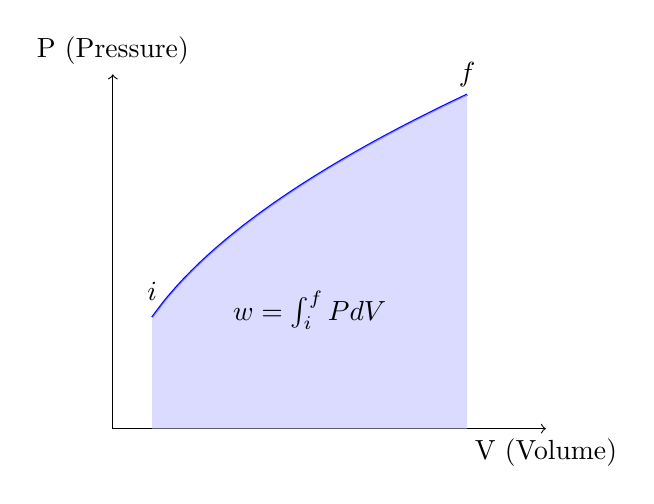
\begin{tikzpicture}
    % Axes
    \draw[->] (0,0) -- (5.5,0) node[below] {V (Volume)};
    \draw[->] (0,0) -- (0,4.5) node[above] {P (Pressure)};
    
    % Curve y = sqrt(4x)
    \draw[thick, blue, domain=0.5:4.5, smooth, variable=\x] 
        plot ({\x}, {(4*\x)^(1/2)});

    % Shade the area under the curve
    \fill[blue!20, opacity=0.7] (0.5,0) -- plot[domain=0.5:4.5] 
        ({\x}, {sqrt(4*\x)}) -- (4.5,0) -- cycle;

    % Label for work (PdV)
    \node[align=center] at (2.5,1.5) {$w = \int_i^f P dV$};
    \node[align=left] at (0.5,1.75) {$i$};
    \node[align=right] at (4.5,4.5) {$f$};
\end{tikzpicture}

\begin{align}
    w &= \int_i^f PdV \\
    w &= \int_i^f PdV + \int_f^i PdV \\
    w &= \Big[\int_i^f PdV\Big]_1 - \Big[\int_i^f PdV \Big]_2 \\
    w &\neq 0 \\
    \Rightarrow \oint_C w &= \oint_C Pdv \neq 0
\end{align}

\begin{align}
    w &= \int_i^f PdV \\
    w &= \int_i^f PdV + \int_f^i PdV \\
    w &= \Big[\int_i^f PdV\Big]_1 - \Big[\int_i^f PdV \Big]_2 \\
    w &= 0 \\
    \Rightarrow \oint_C w &= \oint_C Pdv = 0
\end{align}

\begin{align}
    \delta w &= PAds \\
    \delta w &= F\cdot ds \\ 
    \displaystyle\frac{\delta w}{dt} &= m \frac{dv}{dt} \frac{ds}{dt} \\ 
    \frac{\delta w}{dt} &= mv\frac{dv}{dt} \\ 
    \frac{\delta w}{dt} &= \frac{d}{dt} \Big( \displaystyle\frac{1}{2} mv^2 \Big) \\
    \Rightarrow \frac{\delta w}{dt} &= \frac{d}{dt} (K.E.)
\end{align}

\subsubsection*{Formulation of $1^{st}$ law of thermodynamics}

\textbf{\textit{Case 1:}} Heating
        $$\Delta U = Q$$
\textbf{\textit{Case 2:}} By doing work
        $$\Delta U = -W$$

From case 1 and 2 for we can write $1^{st}$ law of thermodynamics as:
\begin{align}
    \Delta U &= Q - W \\
    \delta q &= du + \delta w
\end{align}

\begin{center}
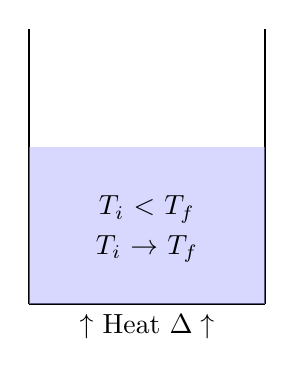
\begin{tikzpicture}
    % Piston cylinder outline (topless)
    \draw[thick] (0, 0) -- (3, 0);  % Closed bottom
    \draw[thick] (0, 0) -- (0, 3.5);  % Left wall
    \draw[thick] (3, 0) -- (3, 3.5);  % Right wall

    % Shaded water region
    \fill[blue!30, opacity=0.5] (0, 0) rectangle (3, 2);  % Water up to dashed line at y=2

    % Dashed lines
    % \draw[dashed, blue] (0, 2) -- (3, 2);
    % \draw[dashed, blue] (0, 1.5) -- (3, 1.5); 
    % \draw[dashed, blue] (0, 1) -- (3, 1);
    % \draw[dashed, blue] (0, 0.5) -- (3, 0.5); 

    % Labels
    \node at (1.5, 0) [below] {$\uparrow$ Heat $\Delta \uparrow$};
    \node at (1.5, 1) [below] {$T_i$ $\rightarrow$ $T_f$};
    \node at (1.5, 1.5) [below] {$T_i$ $<$ $T_f$};
\end{tikzpicture}
\end{center}

In terms of Intensive parameters
\begin{align}
    \delta q &= du + p d\alpha \label{eq:reduced_1st_law_of_thermo}
\end{align}

\begin{enumerate}
    \item Pressuer-volume wok done by a system = reduction in internal energy + heat supplied by the environment.
    \item Pressuer-volume wok done on a system = increase in internal energy + heat transfered to the environment.
\end{enumerate}

\subsection{. Heat capacity}
\begin{equation}
    \displaystyle\frac{\delta q}{dT} =C
    \label{eq:heat_capacity}
\end{equation}
Unit $Jk^{-1}Kg^{-1}$ \\

Ideal gas equation:
$$P \alpha = R_d T$$

\textbf{\textit{Case 1:}} Increase in volume (If pressure is kept constant $\rightarrow$ Isobaric process)

\textbf{\textit{Case 2:}} Increase in pressure (If volume is kept constant $\rightarrow$ Isochoric process)

\textbf{\textit{Case 3:}} Combination of above the both cases. (i.e. increase in both pressure and volume)

\subsection{. Heat capacity at constant volume}
From Eq.\myeqref{eq:reduced_1st_law_of_thermo}
\begin{align}
    \delta q &= du + p d\alpha \\
    \delta q &= du \\
    \delta q &= C_vdT \\
    C_v &= \Big(\frac{\delta q}{dT}\Big)_{\alpha =\text{cont}}\\
    C_v &= \Big(\frac{du}{dT}\Big)_{\alpha =\text{cont}}\\
    \Rightarrow du &= C_vdt
\end{align}

From Kinetic theory of gas
$$ U = \frac{3}{2}P\alpha = \frac{3}{2}R_dT$$
For monoatomic gas:
$$C_v = \frac{du}{dt} = \frac{3}{2}R_d = 430.5 Jk^{-1}kg^{-1}$$ 
For diatomic gas:
$$C_v = \frac{du}{dt} = \frac{5}{2}R_d = 718 Jk^{-1}kg^{-1}$$

% NOTE: COMPLETED L-10
% --------------------------------------------------------------------------------------
\clearpage

\section{Lecture 11 06/09/2024}

\subsection{. Specific heat capacity}
Specific heat = $\frac{\delta q}{dT}$
\begin{align}
    \delta q = du + \delta w \\ 
    \delta q = du + p d \alpha 
\end{align}

\subsection{. Specific heat at constant volume}
Volume($V$) is constant ,i.e., specific density($\alpha$) = constant 

$\therefore$ $d \alpha = 0$
\begin{align}
    \delta q &= du + p d\alpha \\
    \delta q &= du \\
    \delta q &= C_vdT \\
    C_v &= \Big(\frac{\delta q}{dT}\Big)_{\alpha =\text{cont}}\\
    C_v &= \Big(\frac{du}{dT}\Big)_{\alpha =\text{cont}}\\
    du &= C_vdt
\end{align}

Hence,
\begin{align}
   \Rightarrow \delta q = C_vdt + Pd\alpha     \label{eq:1st_law_with_const_volume}
\end{align}

\begin{align*}
C_v = 
    \begin{cases} 
        \frac{3}{2} R_d & \text{for monoatomic gas}, \\
        \frac{5}{2} R_d & \text{for diatomic gas}.
    \end{cases}
\end{align*}

Rotational K.E. is significant for diaatomic gas but not for monoatomic gas.

\begin{center}
% Monoatomic Gas
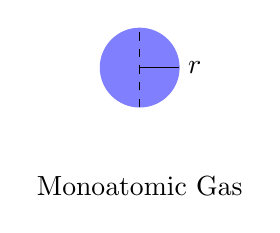
\begin{tikzpicture}
    % Single atom
    \filldraw[blue!50] (0, 0) circle (0.5);
    \draw[dashed] (0, -0.5) -- (0, 0.5);  % Vertical line through the center
    
    % Radius indication
    \draw[-] (0, 0) -- (0.5,0);
    \node at (0.7, 0) {$r$};  % Radius label
    
    % Label for monoatomic gas
    \node at (0, -1.5) {Monoatomic Gas};
\end{tikzpicture}
\hspace{2cm}
% Diatomic Gas
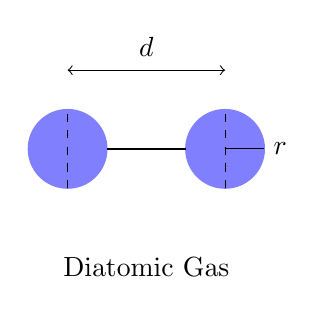
\begin{tikzpicture}
    % First atom
    \filldraw[blue!50] (0, 0) circle (0.5);
    % Second atom
    \filldraw[blue!50] (2, 0) circle (0.5);
    
    % Bond between atoms
    \draw[thick] (0.5, 0) -- (1.5, 0);
    
    % Vertical lines through the centers of the atoms
    \draw[dashed] (0, -0.5) -- (0, 0.5);
    \draw[dashed] (2, -0.5) -- (2, 0.5);
    
    % Distance between the centers of the atoms
    \draw[<->] (0, 1) -- (2, 1);
    \node at (1, 1.3) {$d$};  % Distance label
    
    % Radius indication
    \draw[-] (2, 0) -- (2.5,0);
    \node at (2.7, 0) {$r$};  % Radius label
    
    % Label for diatomic gas
    \node at (1, -1.5) {Diatomic Gas};
\end{tikzpicture}
\hspace{2cm}
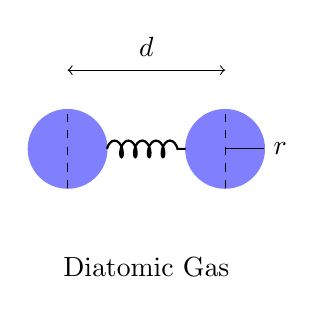
\begin{tikzpicture}
    % First atom
    \filldraw[blue!50] (0, 0) circle (0.5);
    % Second atom
    \filldraw[blue!50] (2, 0) circle (0.5);
    
    % Spring (wavy line) between the atoms
    \draw[thick,decorate,decoration={coil,aspect=0.5,segment length=5pt,amplitude=3pt}] (0.5,0) -- (1.5,0);
    
    % Vertical lines through the centers of the atoms
    \draw[dashed] (0, -0.5) -- (0, 0.5);
    \draw[dashed] (2, -0.5) -- (2, 0.5);
    
    % Distance between the centers of the atoms
    \draw[<->] (0, 1) -- (2, 1);
    \node at (1, 1.3) {$d$};  % Distance label
    
    % Radius indication
    \draw[-] (2, 0) -- (2.5,0);
    \node at (2.7, 0) {$r$};  % Radius label
    
    % Label for diatomic gas
    \node at (1, -1.5) {Diatomic Gas};
\end{tikzpicture}
\end{center}

\subsection{. Specific heat at constant pressure}
Pressure($P$) is constant 
$\therefore$ $dP = 0$

From Ideal gas eqaution
\begin{align}
    P\alpga &= R_d T \\ 
    dP \alpha &= Pd\alpha + \alpha dP \\ 
    Pd\alpha + \alpha dP &= d(R_d T) \\
    Pd\alpha + \alpha dP &= R_d dT \\
    Pd\alpha  &= R_d dT - \alpha dP \label{eq:p_d_alpha}
\end{align}
\begin{align}
    \delta q &= du + p d\alpha \\
    \delta q &= du \\
    \delta q &= C_vdT \\
    C_v &= \Big(\frac{\delta q}{dT}\Big)_{\alpha =\text{cont}}\\
    C_v &= \Big(\frac{du}{dT}\Big)_{\alpha =\text{cont}}\\
    du &= C_vdt
\end{align}

From Eq.\myeqref{eq:1st_law_with_const_volume} and Eq.\myeqref{eq:p_d_alpha} 
\begin{align}
    \delta q &= C_vdT + R_ddT-\alpha dP \\ 
    \delta q &= (C_v + R_d)dT-\alpha dP \\ 
    \Rightarrow \delta q &= C_pdT-\alpha dP
\end{align}

\begin{align*}
C_p =
    \begin{cases}
        717.5 \, \text{J} \cdot \text{kg}^{-1} \cdot \text{K}^{-1} & \text{for monoatomic gas} \\
        1005 \, \text{J} \cdot \text{kg}^{-1} \cdot \text{K}^{-1} & \text{for diatomic gas}
    \end{cases}
\end{align*}

\subsection{. Special forms of 1$^{st}$ laaw of thermodynamics}
\subsubsection*{I. Isobaric process}
\begin{align}
    \delta q &= C_p dT \\
             &= \Big(\frac{C_p}{C_v}\Big)C_v dT \\
             &= \Big(\frac{C_p}{C_v}\Big) dU \\
             &= \gamma dU
\end{align}

\subsubsection*{II. Isothermal process}
\begin{align}
    \delta q &= -\alpha dP = Pd\alpha = \delta w \\
    q &= \int^f_i \alpha dP \\
      &= \int^f_i \frac{R_d T}{P} dP \\
      &= -R_d T \ln P|^f_i \\
      &= -R_d T \ln P|^f_i \\
      &= R_d T \ln \alpha|^f_i = w \\
\end{align}

\subsubsection*{III. Isochoric process}
\begin{align}
    \delta q &= C_v dT =du  d\alpha = 0 \\
    q &= \int^f_i C_v dT \\
      &= C_v (T_f -T_i) \\
      &= C_v \Delta T = U
\end{align}

\subsubsection*{IV. Adiabatic process}
\begin{align}
    0 &= C_v dT + P\alpha \\
    %C_v dT &= -P\alpha \\
    0 &= C_p dT - P\alpha
    %C_p dT &= -\alpha dP
\end{align}

\begin{question}[label=q11.1]{For each of the following conditions compute: \newline
     i. Mechanical work done by the sample of air. \newline
     ii. Heat added to the sample. \newline
     a. Isothermal cpmpression to $1/5^{th}$ of it's original volume at $15^{\circ}C$. \newline
     b. Isobaric heating from $0^{\circ}C$ to $20^{\circ}C$.\newline
     c. Adiabatic expansion to $5$ times it's orignanal volume within initial temperature of $20^{\circ}C$.
}
$\Rightarrow$ Solution:

a. For Isothermal process
\begin{align*}
    q = w &= R_d T \ln\Big(\frac{1}{V}\Big)\Big|^{V/5}_{V}\\
          &= 287 \times 288 \times T \ln(5) \\
          &= 133.0297 kJ 
\end{align*}

b. For Isobaric heating
\begin{align*}
    q &= C_p dT \\
      &= \frac{7}{2} R_d \times \Delta T \\
      &= \frac{7}{2} \times 287 \times 20 \\
      &= 19740 J \\
      &\approx 20 kJ
\end{align*}
c. Adiabatic heating
\begin{align*}
    % T_1 &= 293K \\
    % T_2 &= \frac{V_1}{V_2}T_1 = \frac{1}{5} \times 293 \\
    w &= \frac{P_1V_1 - P_2V_2}{\gamma -1} \\
      &= \frac{R_d (T_1 -T_2)}{\gamma -1} \\
      & = \frac{287 \times (293 - \frac{293}{5})}{\frac{7}{5} -1} \\
      &= 168.182 kJ \\
    q &= 0 J
\end{align*}
\end{question}

% NOTE: COMPLETED L-11
% --------------------------------------------------------------------------------------
\clearpage

\section{Lecture 12 11/09/2024}
\subsection{. Poisson's equation for adiabatic transformation}
For adiabatic processes:
\begin{align}
    dq &= 0 \\
    c_p dT &= \alpha dP \\
    c_p \frac{dT}{T} &= \alpha \frac{dP}{T} \\
\end{align}
From Ideal gas equations:
\begin{align}
    P\alpha &= R_dT \\
    \alpha &= \frac{R_d T}{P}
\end{align}
\begin{align}
    c_p \frac{dT}{T} &= \frac{R_d T}{P} \frac{dP}{T} \\
    c_p \frac{dT}{T} &= R_d \frac{dP}{P}
\end{align}
Integrating from an initial termerature $T_0$ and pressure $P_0$ to arbitary temperature and pressure $T$ and $P$
\begin{align}
    \int^{T}_{T_0} c_p \frac{dT}{T} &= \int^{P}_{P_0} R_d \frac{dP}{P} \\
    c_p \ln\Big(\frac{T}{T_0}\Big) &= R_d  \ln\Big(\frac{P}{P_0}\Big) \\
    \Big(\frac{T}{T_0}\Big)^{c_p} &= \Big(\frac{P}{P_0}\Big)^{R_d} \\
    T_0 &= T\Big(\frac{P}{P_0}\Big)^{\frac{R_d}{c_p}} \\
    \Rightarrow \theta &= T\Big(\frac{1000}{P_0}\Big)^{k} \label{eq:poissonsEq}
\end{align}
where constant $k$ is $R_d/c_p$ which is equal to \textbf{0.286}, $P_0 = 1000 hPa$ which is \textbf{near surface pressure} and $\theta$ is known as \textbf{potential temperature}. \\
$\theta$ known as \textbf{potential temperature} Eq.\myeqref{eq:poissonsEq} is defined when a adiabaticatly compressed parcel and bought to $1000hPa$ isobar (near surface) and temperature is measure. \\

\newpage
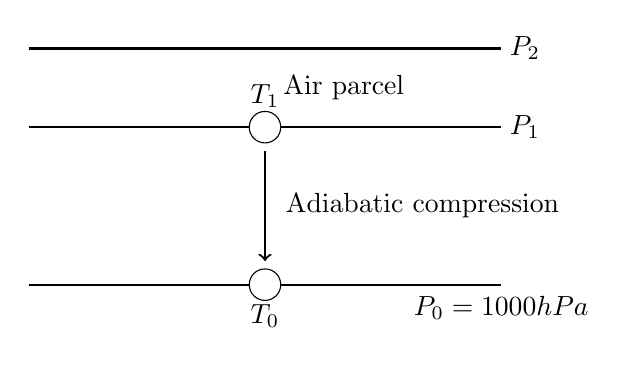
\begin{tikzpicture}
    % Draw three horizontal lines
    \draw[thick] (0,0) -- (6,0);   % First line
    \draw[thick] (0,-1) -- (6,-1); % Second line
    \draw[thick] (0,-3) -- (6,-3); % Third line

    % Draw circles on the second and third lines
    \draw[fill=white] (3,-1) circle [radius=0.2]; % Circle at (3, -1)
    \draw[fill=white] (3,-3) circle [radius=0.2]; % Circle at (3, -3)

    % Label the circles
    \node at (4,-0.5) {$\text{Air parcel}$};
    \node at (5,-2) {$\text{Adiabatic compression}$};
    \node at (3,-0.6) {$T_1$};
    \node at (3,-3.4) {$T_0$};
    \node at (6.3,-0) {$P_2$};
    \node at (6.3,-1) {$P_1$};
    \node at (6,-3.3) {$P_0 = 1000 hPa$};

    % Draw downward arrow from second to third line
    \draw[->, thick] (3,-1.3) -- (3,-2.7);
\end{tikzpicture}

Let us assume that 

\begin{align}
    \theta &= ATP^{-k}
\end{align}
taking logorithm on both sides
\begin{align}
    d(\ln \theta) &= d(\ln A) + d(\ln T) - kd(\ln P) \\
    d(\ln \theta) &= d(\ln T) - \frac{R_d}{C_p}d(\ln P) \label{eq:potential_temperature_1}
\end{align}
where $A = (P_0)^k = (1000)^{0.286}$

Consider $1^{st}$ law of thermodynamics
\begin{align}
    \delta q &= C_p dT - \alpha dP \\
    \frac{\delta q}{T} &= C_p\frac{dT}{T} - \alpha\frac{dP}{T} \\
    \frac{\delta q}{C_p T} &= \frac{dT}{T} - \frac{R_d T dP}{C_p PT} \\
    \frac{\delta q}{C_p T} &= \frac{dT}{T} - \frac{R_d dP}{C_p P} \\
    \frac{\delta q}{C_p T} &= d(\ln T) - \frac{R_d}{C_p} d(\ln P) \label{eq:potential_temperature_2}
\end{align}

from Eq.\myeqref{eq:potential_temperature_1} and Eq,\myeqref{eq:potential_temperature_2}
\begin{align}
    d(\ln \theta) = \frac{\delta q}{C_p T}
\end{align}

For adiabatic process $\delta q=0$
\begin{align}
    d(\ln \theta) = 0
\end{align}
$\theta$ is constant, conserved for adiabatic process.

\begin{question}[q:12.1]{Transcontinental airline flys at an altitude of 12km where the temperature outside is $-55^{\circ}C$ and the pressure is approxiately 200hPa \newline
    a. Compute the potential temperature of air at this altitude. \newline
    b. Cabin pressure is typically mentioned of $750 hPa$ corresponding to pressure alttitude of $2.24$km. when outside air is adiabatically compressed to cabin pressure, compute the air temperature if no corrective operation where taken.
}
$\Rightarrow$ Solution:

a. \begin{align*}
    \theta &= T \Big(\frac{1000}{P}\Big)^k \\ 
           &= 218 \Big(\frac{1000}{200}\Big)^{0.286}\\ 
           &= 218 (5)^{0.286}\\ 
           &= 345.4317 K \\
           &= 72.43 ^\circ C
\end{align*}

b. \begin{align*}
    \theta &= T \Big(\frac{1000}{P}\Big)^k \\ 
           &= 218 \Big(\frac{750}{200}\Big)^{0.286}\\ 
           &= 218 \Big(\frac{4}{3}\Big)^{0.286}\\ 
           &= 318.14 K \\
           &= 45 ^\circ C
\end{align*}
\end{question}

% NOTE: COMPLETED L-12
% --------------------------------------------------------------------------------------
\clearpage

\section{Lecture 13 12/09/2024}
\subsection{. Adiabatic transformation - Poisson's equation}

\begin{enumerate}
    \item Case I. 
        \begin{align}
            C_p dT &= \alpha dP  \\
            C_p \frac{dT}{T} &= R_d \frac{dP}{P}  \\
            \frac{dT}{T} &= \Big(\frac{C_p - C_v}{C_p}\Big) \frac{dP}{P}  \\
            \frac{dT}{T} &= \Big(1 - \frac{C_v}{C_p}\Big) \frac{dP}{P}  \\
            \frac{dT}{T} &= \Big(1 - \frac{1}{\gamma}\Big) \frac{dP}{P}  \\
            \frac{dT}{T} &= \Big(\frac{\gamma - 1}{\gamma}\Big) \frac{dP}{P} \\
            \ln T &= \Big(\frac{\gamma - 1}{\gamma}\Big) \ln P + \ln C \\
            T &= CP^{\Big(\frac{\gamma - 1}{\gamma}\Big)} \\
            T P^{\Big(\frac{1 - \gamma}{\gamma}\Big)} &= C
        \end{align}
    \item Case II. 
        \begin{align}
            C_v dT &= -P d\alpha  \\
            C_v \frac{dT}{T} &= -R_d \frac{d\alpha}{\alpha}  \\
            \frac{dT}{T} &= -\Big(\frac{C_p - C_v}{C_v}\Big) \frac{d\alpha}{\alpha} \\
            \frac{dT}{T} &= \Big(1 - \frac{C_p}{C_v}\Big) \frac{d\alpha}{\alpha} \\
            \frac{dT}{T} &= \Big(1 - \gamma\Big) \frac{d\alpha}{\alpha} \\
            \ln T &= (1 - \gamma)\ln \alpha + \ln C \\
            \ln T &= \ln \alpha^{(1 - \gamma)} + \ln C \\
            T &= C\alpha^{(1-\gamma)} \\
            T\alpha^{(\gamma - 1)} &= C
\end{align}
\end{enumerate}

\subsection{. Adiabatic Lapse Rate}
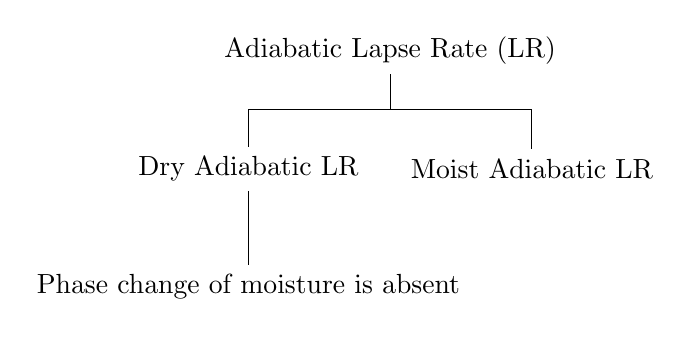
\begin{tikzpicture}[
  edge from parent fork down,
  sibling distance=2cm, % Adjust sibling distance
  level 1/.style={sibling distance=3.6cm, level distance=1.5cm}, % First level
  level 2/.style={sibling distance=1cm} % Second level
]
% Define the tree structure
\node {Adiabatic Lapse Rate (LR)}
    child { node {Dry Adiabatic LR}
        child {node {Phase change of moisture is absent}}
    }
    child { node {Moist Adiabatic LR} };
\end{tikzpicture}
\end{center}

\textbf{Note:} Moisture is present in dry air parcel but it is assumed that it does not show any phase chage.

\subsection{. Dry Adiabatic Lapse Rate (DALR)}
Using the $1^{st}$ law of thermodynamics 
\begin{equation}
    \delta q = C_pdT - \alpha dP 
\end{equation}

Adiabatic process
\begin{align}
    \delta q &= 0 \\
    C_p dT &= \alpha dP \label{eq:C_pdT=adp}
\end{align}

Lapse rate
\begin{align}
    \frac{dT}{dz} &= \frac{dT}{dP} \frac{dP}{dz} \label{eq:dTdz=dtdpdpdz}
\end{align}

From Eq.\myeqref{eq:C_pdT=adp} and \myeqref{eq:dTdz=dtdpdpdz}
\begin{align}
    \frac{dT}{dz} &= \frac{R_d T}{C_p P} \frac{dP}{dz} \label{eq:dTdz}
\end{align}

\textbf{Note:} Hydrostatic balance is applied to surrounding not on parcel.

Appling hydrostatic approximaion, The pressure of unconfined air pacel is same as that of the envirnoment, we get:
\begin{align}
    \frac{dP}{dz} = \frac{dP'}{dz} = \rho'g = -\frac{P'g}{R_d T'} \label{eq:dPdz}
\end{align}
where $P'$ and $T'$ are ambient pressure and temperature.

From Eq.\myeqref{eq:C_pdT=adp}, Eq.\myeqref{eq:dTdz=dtdpdpdz} and \myeqref{eq:dPdz}
\begin{align}
    \frac{dT}{dz} &= \frac{R_dT}{C_pP} \times \Big(- \frac{P'g}{R_dT'} \Big) \\
    \frac{dT}{dz} &= \frac{g}{C_p} \times \Big(- \frac{TP'}{T'P} \Big)\\
    \frac{dT}{dz} &= -\frac{g}{C_p}\Big(\frac{T}{T'} \Big) \\
    \Gamma_d = -\frac{dT}{dz} &= \frac{g}{C_p}\Big(\frac{T}{T'} \Big) \\
    \Gamma_d = -\frac{dT}{dz} &\approx \frac{g}{C_p}\\
    \Gamma_d = -\frac{dT}{dz} &\approx 9.8\times 10^{-3}^{\circ}C/m \\
    \Rightarrow \Gamma_d = -\frac{dT}{dz} &\approx 9.8^{\circ}C/km
\end{align}
where $\Gamma_d$ is \textbf{Dry Adiabatic Lapse Rate (DALR)} which is aproximately equal to $9.8^{\circ}C/km$, also $T$ and $T'$ are comparably equal.

\subsection{. Possion's equations}
From Eq.\myeqref{eq:poissonsEq}
\begin{align}
    \theta &= T\Big(\frac{1000}{P}\Big)^k \\
    \Rightarrow P^k &= \Big(\frac{P_0^k}{\theta}\Big)T
\end{align}

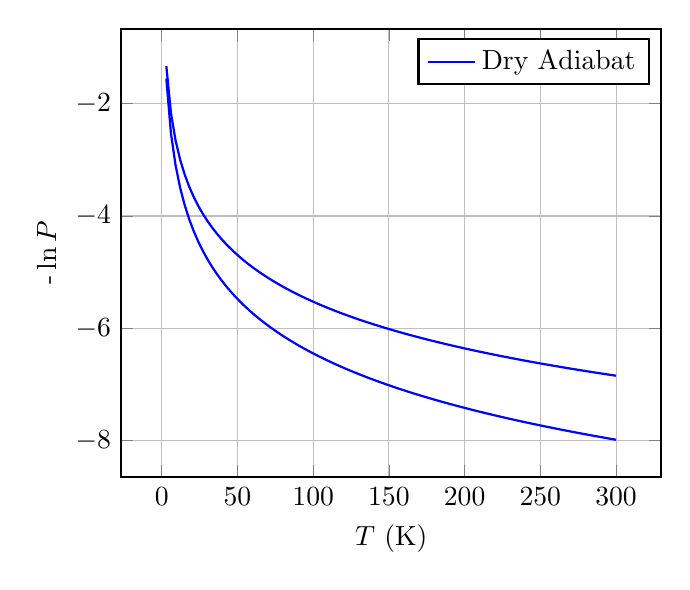
\begin{tikzpicture}
  \begin{axis}[
    xlabel={$T$ (K)},
    ylabel={$\text{-}\ln P$},
    domain=0:300, % Temperature range
    samples=100,
    grid=both,
    minor grid style={gray!25},
    major grid style={gray!50},
    thick
  ]
    % Equation for dry adiabat, approximated here
    \addplot[blue, thick] {ln(x^(-1.4))};
    \addplot[blue, thick] {ln(x^(-1.2))};
    \addlegendentry{Dry Adiabat}
  \end{axis}
\end{tikzpicture}

% NOTE: COMPLETED L-13
% --------------------------------------------------------------------------------------
\clearpage

\section{Lecture 14 20/09/2024}

\subsection{. Heat Engines}
\begin{enumerate}
    \item Construct closed cycle of compression and expansion to produce net work.
    \item Production of work required expenditure of internal energy on heat supplied by the environment.
\end{enumerate}

From 1$^{st}$ law of thermodynamics
\begin{align}
    \delta q &= du + \delta w \\
    \oint \delta q &= \oint du + \oint \delta w \\
    \oint \delta q &= \oint \overset{0}{\cancel{du}} + \oint \delta w \quad \text{(} \because u_i = u_f\text{)} \\
    \oint \delta q &= \oint \delta w \\
    \Rightarrow q_{\text{net}} &= w_{\text{net}} \quad \text{(Theoritically)}
\end{align}

In theory, the equality \( q_{\text{net}} = w_{\text{net}} \) arises from the assumption of a perfect heat engine operating in a closed cycle. This idealized scenario implies that all the heat energy supplied to the engine is converted into mechanical work without any losses due to friction, heat dissipation, or other irreversibilities.

However, no physical engine can achieve this ideal efficiency. Real engines inevitably encounter energy losses through various mechanisms, such as:

\begin{enumerate}
    \item \textbf{Heat Loss:} Part of the input heat is lost to the surroundings, decreasing the effective energy available for work.
    \item \textbf{Friction:} Mechanical losses due to friction in moving parts result in energy dissipation as heat, further reducing the net work output.
    \item \textbf{Non-ideal Processes:} Real thermodynamic processes often involve irreversible changes, which lead to additional energy losses that are not accounted for in the ideal model.
\end{enumerate}

Thus, while \( q_{\text{net}} = w_{\text{net}} \) serves as a theoretical benchmark, practical engines operate with efficiencies below this ideal, governed by real-world constraints and inefficiencies.

\subsection{. Efficiency}
Efficiency of heat engine,
\begin{equation}
\eta = \frac{q_\text{in}-q_{\text{out}}}{q_{\text{in}}} = \frac{w}{q_{\text{in}}}
    \label{eq:effiency}
\end{equation}

\subsection{. Carnot Cycle}

The Carnot cycle consists of the following four steps, whcih can be seen in figure:
\begin{enumerate}[noitemsep]
    \item \textbf{Step 1:} Reversible isothermal expansion.
    \item \textbf{Step 2:} Reversible adiabatic expansion.
    \item \textbf{Step 3:} Reversible isothermal compression.
    \item \textbf{Step 4:} Reversible adiabatic compression.
\end{enumerate}

\begin{figure}[ht]
    \begin{center}
        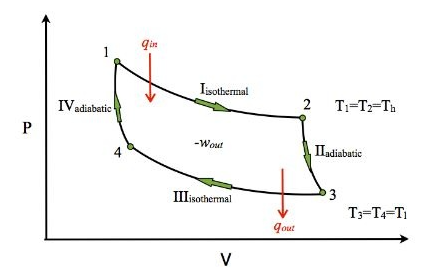
\includegraphics[width=0.5\textwidth]{Figures/Carnot_cycle.png}
    \end{center}
    \caption{Carnot Cycle}\label{fig:carnot_cycle}
\end{figure}

\textbf{Step 1: Reversible Isothermal Expansion}

During this process, the temperature remains constant, i.e., \( \Delta T = 0 \), which implies that the internal energy change is zero, \( \Delta u = 0 \).

The work done during this process is given by:
\begin{align}
    w_{12} &= \int \delta w = \int_{\alpha_1}^{\alpha_2} p \, d\alpha \\
    &= \int_{\alpha_1}^{\alpha_2} \frac{R_d T_1}{\alpha} \, d\alpha \\
    &= R_d T_1 \ln \frac{\alpha_2}{\alpha_1} \label{eq:w12}
\end{align}

Since $du = 0$ (because $dT = 0$), we have:
$$
du_{12} = dw_{12} \quad \Rightarrow \quad Q_{12} = W_{12}
$$ 

\textbf{Step 2: Reversible Adiabatic Expansion}

In this step, the gas expands without heat exchange, leading to a change in internal energy. The change in internal energy is given by:
\begin{align}
    \Delta u_{23} &= C_v(T_2 - T_1) \\
    -\Delta u_{23} &= w_{23} \\
    w_{23} &= -C_v(T_2 - T_1) \label{eq:w23}
\end{align}

\textbf{Step 3: Reversible Isothermal Compression}

In this process, the gas is compressed isothermally, maintaining a constant temperature:
\begin{align}
    w_{34} &= \int \delta w = \int_{\alpha_3}^{\alpha_4} p \, d\alpha \\
    &= \int_{\alpha_3}^{\alpha_4} \frac{R_d T_2}{\alpha} \, d\alpha \\
    &= R_d T_2 \ln \frac{\alpha_4}{\alpha_3} \label{eq:w34}
\end{align}

\textbf{Step 4: Reversible Adiabatic Compression}

During this step, the gas is compressed adiabatically, resulting in a temperature increase and work done on the gas. The work can be expressed as:
\begin{align}
    w_{41} &= C_v(T_2 - T_1) \label{eq:w41}
\end{align}

From Poisson's equation \myeqref{eq:poissonsEq}, we have the following relations for the Carnot cycle:
\begin{align}
    T_1 \alpha_2^{\gamma - 1} &= T_2 \alpha_3^{\gamma - 1} \\
    \frac{T_1}{T_2} &= \left(\frac{\alpha_3}{\alpha_2}\right)^{\gamma - 1}
\end{align}

Similarly, for the other isentropic process:

\begin{align}
    T_1 \alpha_1^{\gamma - 1} &= T_2 \alpha_4^{\gamma - 1} \\
    \frac{T_1}{T_2} &= \left(\frac{\alpha_4}{\alpha_1}\right)^{\gamma - 1}
\end{align}

From these two equations, we can equate the temperature ratios:

\begin{align}
    \left(\frac{\alpha_3}{\alpha_2}\right)^{\gamma - 1} &= \left(\frac{\alpha_4}{\alpha_1}\right)^{\gamma - 1} \\
    \frac{\alpha_3}{\alpha_4} &= \frac{\alpha_2}{\alpha_1} \label{eq:volume_ratio}
\end{align} \\
\textbf{Total Work:}

From Eq.\myeqref{eq:w12}, \myeqref{eq:w23}, \myeqref{eq:w34}, and \myeqref{eq:w41}, the total work done in the cycle is:
\begin{align}
    W_{\text{Total}} &= w_{12} + w_{23} + w_{34} + w_{41} \\
                     &= R_d T_1 \ln \frac{\alpha_2}{\alpha_1} - C_v(T_2 - T_1) + \\ 
                     & \quad  R_d T_2 \ln \frac{\alpha_4}{\alpha_3} + C_v(T_2 - T_1) \\
                     &=  R_d T_1 \ln \frac{\alpha_2}{\alpha_1} + R_d T_2 \ln \frac{\alpha_4}{\alpha_3} \\
                     &= R_d \Big[T_1 \ln \frac{\alpha_2}{\alpha_1} + T_2 \ln \frac{\alpha_4}{\alpha_3} \Big] \\
                     &= R_d(T_1 - T_2) \ln\Big(\frac{\alpha_2}{\alpha_1}\Big) \quad \text{From Eq.\myeqref{eq:volume_ratio}} \label{eq:TotalWorkDone}
\end{align}

Finding the effeincy of carnot cycle using Eq.\myeqref{eq:effiency} and Eq\myeqref{eq:TotalWorkDone}
\begin{align}
    \eta & = \frac{Q_1 + Q_2}{Q_1} \\
        &= 1 + \frac{Q_2}{Q_1} \\
        &= 1 + \frac{R_d T_2 \ln\frac{\alpha_3}{\alpha_4}}{R_d T_1 \ln\frac{\alpha_2}{\alpha_1}} \\
        &= 1 - \frac{T_2 \ln\frac{\alpha_2}{\alpha_1}}{T_1 \ln\frac{\alpha_2}{\alpha_1}} \\
     \Rightarrow \eta &= 1 - \frac{T_2}{T_1} \label{eq:eff_carnot}
\end{align}

The temperature at which carnot engine becomes $100\%$ efficient (i.e.$\eta=1$) is called \textbf{Absolute temeperature ($0K$)} 

In real world scenarios $0K$ is not acheivable and there is no process which is ideally reversible.

\begin{question}[\label=14.1]{For a potential temperature of $290K$ compute the corresponding temperature at $700hPa$ and $500hPa$. Sketch the corresponding adiabat in skew-T diagram.}
    \Rightarrow 
        \theta &= T\Big(\frac{1000}{P_0}\Big)^k  \quad ,\text{where } k=\frac{R_d}{C_p}=\frac{287}{1004}=0.286 \\
        T     &= \theta \Big(\frac{P_0}{1000}\Big)^k \\
        T_1   &= \theta \Big(\frac{700}{1000}\Big)^{0.286} = 261.87K \approx -11.2^\circ C \\
        T_2   &= \theta \Big(\frac{500}{1000}\Big)^{0.286} = 237.88K \approx -35.15^\circ C
\end{question}

\subsection{. Skew T - log P diagram}
\myhref{https://www.noaa.gov/jetstream/upperair/skew-t-log-p-diagrams}{Skew-T plot} shows combined and also seperate plots for Full Skew-T, Isothermal lines, Isobars, Dry Adiabats, Moist Adiabats, Mixing Ratio and Wind Staff.

% \begin{figure*}[ht]\centering
% 	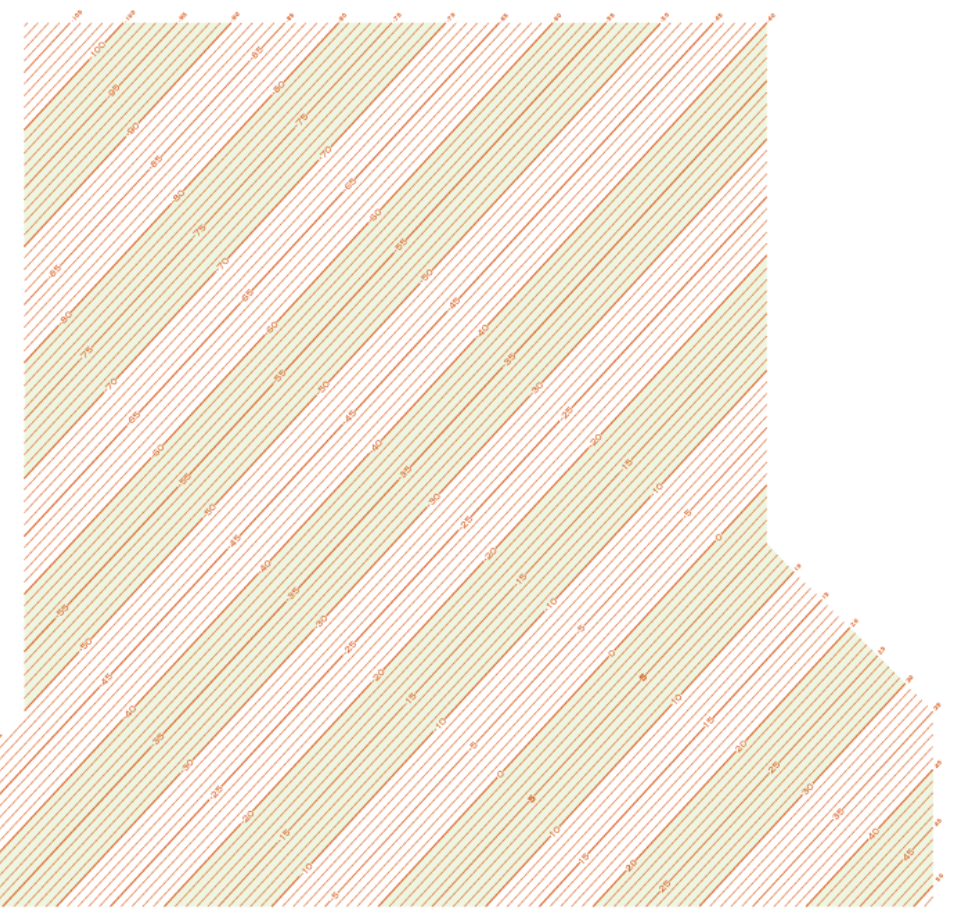
\includegraphics[width=0.6\textwidth]{Figures/Iso-thermal-lines.png}
%         \caption{Isothermal lines in Skew-T diagram}
% \end{figure*}
% \begin{figure*}[ht]\centering
% 	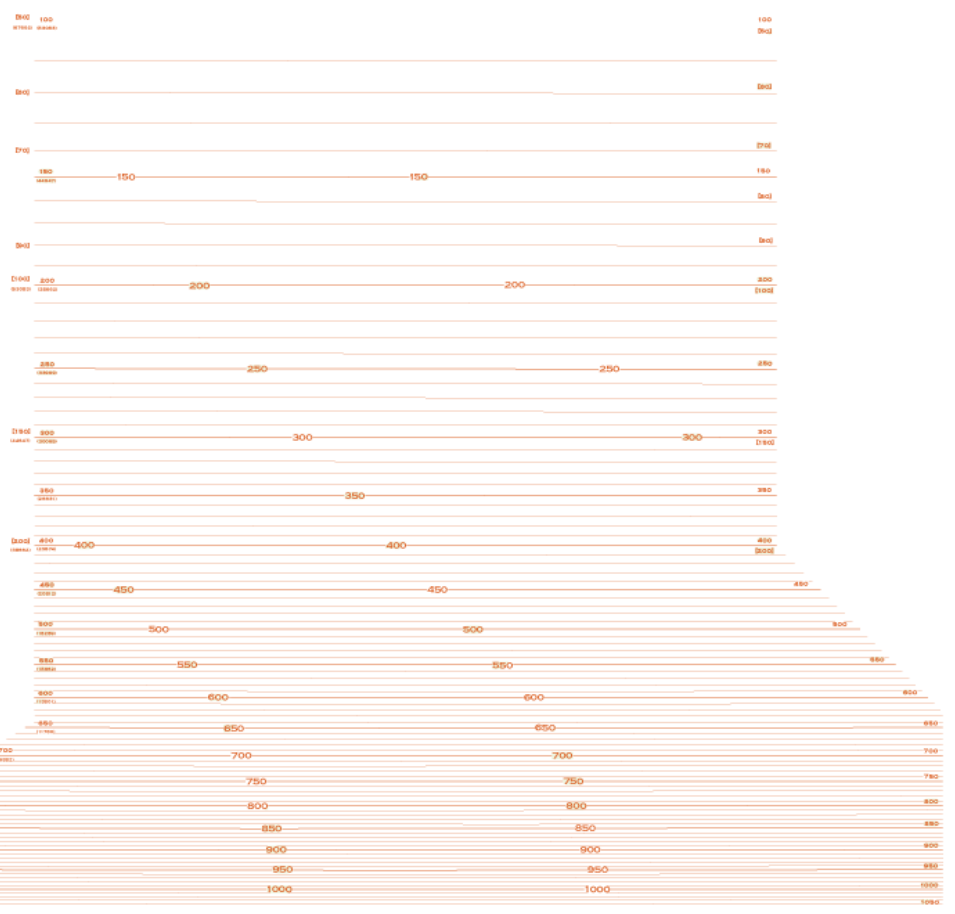
\includegraphics[width=0.6\textwidth]{Figures/Iso-baric-lines.png}
%         \caption{Isobaric lines in Skew-T diagram}
% \end{figure*}
% \begin{figure*}[ht]\centering
% 	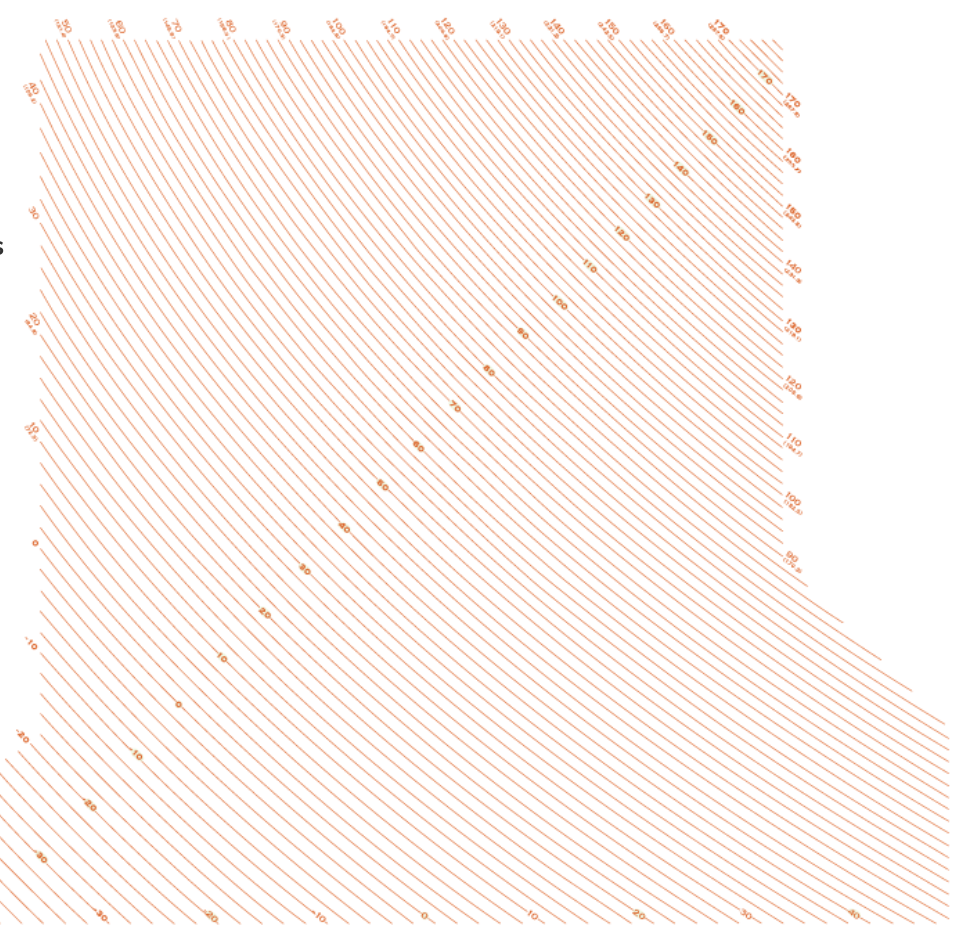
\includegraphics[width=0.6\textwidth]{Figures/Dry-adiabat-lines.png}
%         \caption{Dry-adiabat lines in Skew-T diagram}
% \end{figure*}
% \begin{figure*}[ht]\centering
% 	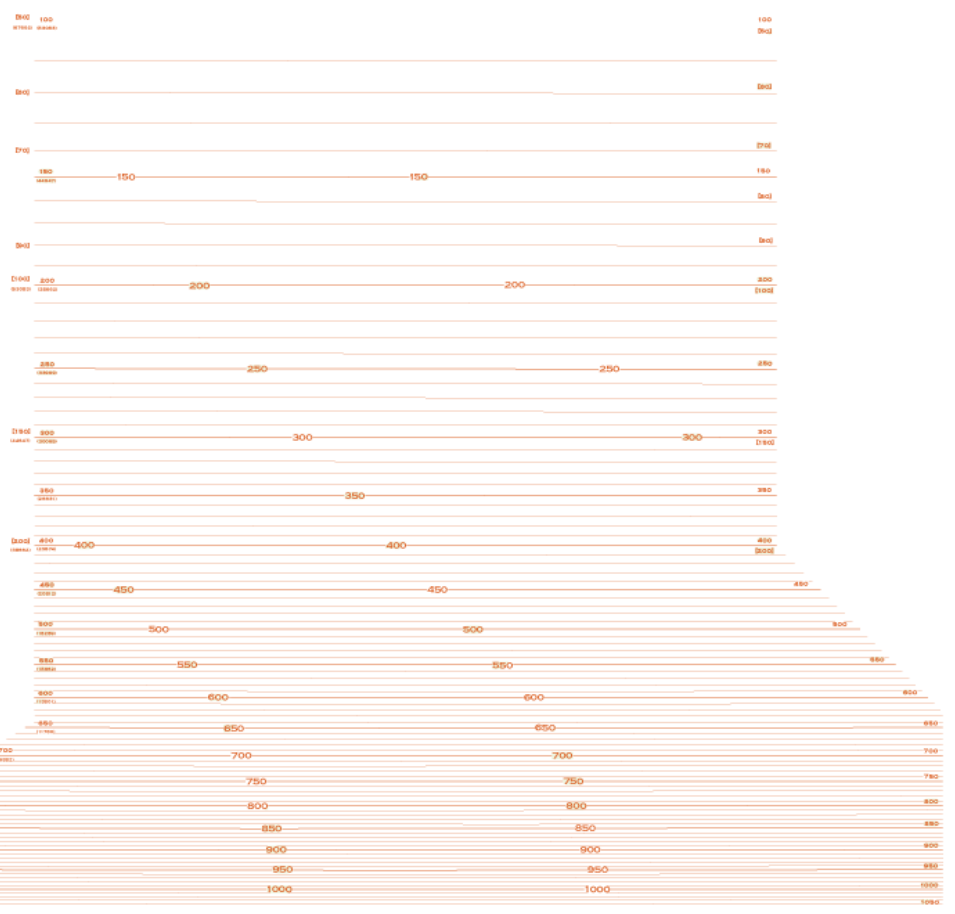
\includegraphics[width=0.6\textwidth]{Figures/Iso-baric-lines.png}
%         \caption{Isobaric lines in Skew-T diagram}
% \end{figure*}
% \begin{figure*}[ht]\centering
% 	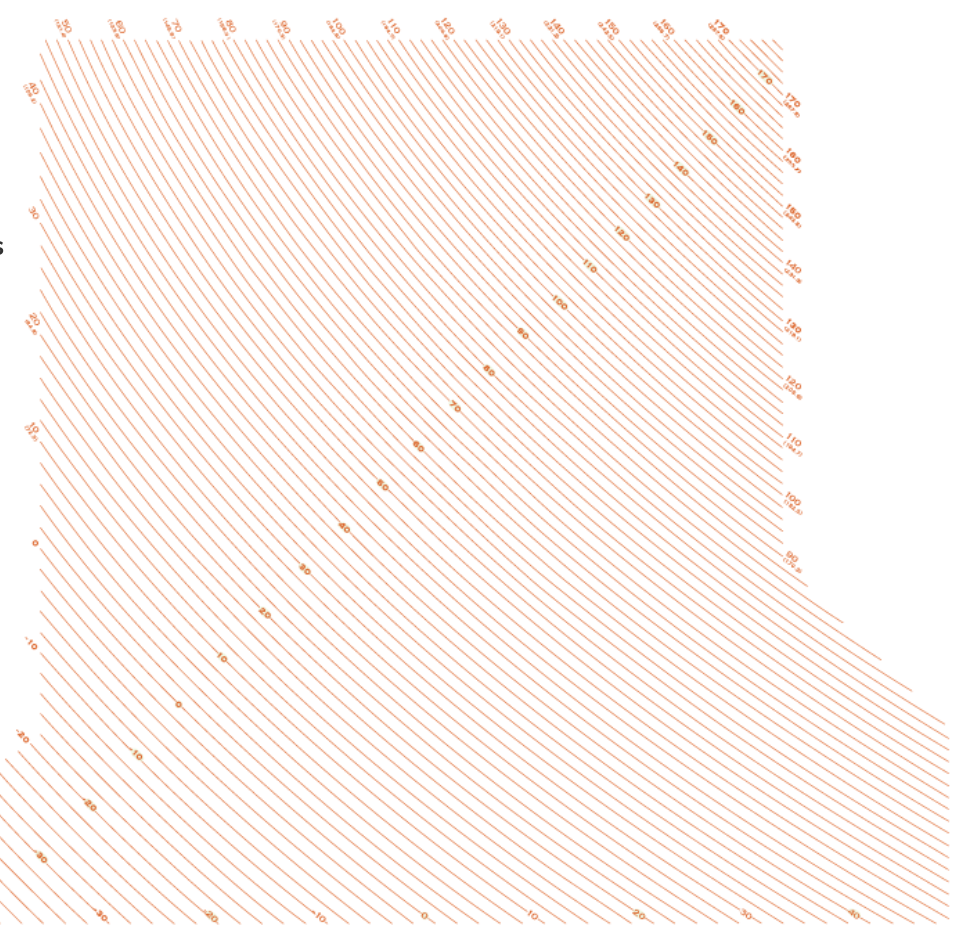
\includegraphics[width=0.6\textwidth]{Figures/Dry-adiabat-lines.png}
%         \caption{Dry-adiabat lines in Skew-T diagram}
% \end{figure*}

\begin{figure*}[ht]
    \centering
    \begin{minipage}[b]{0.48\textwidth}
        \centering
        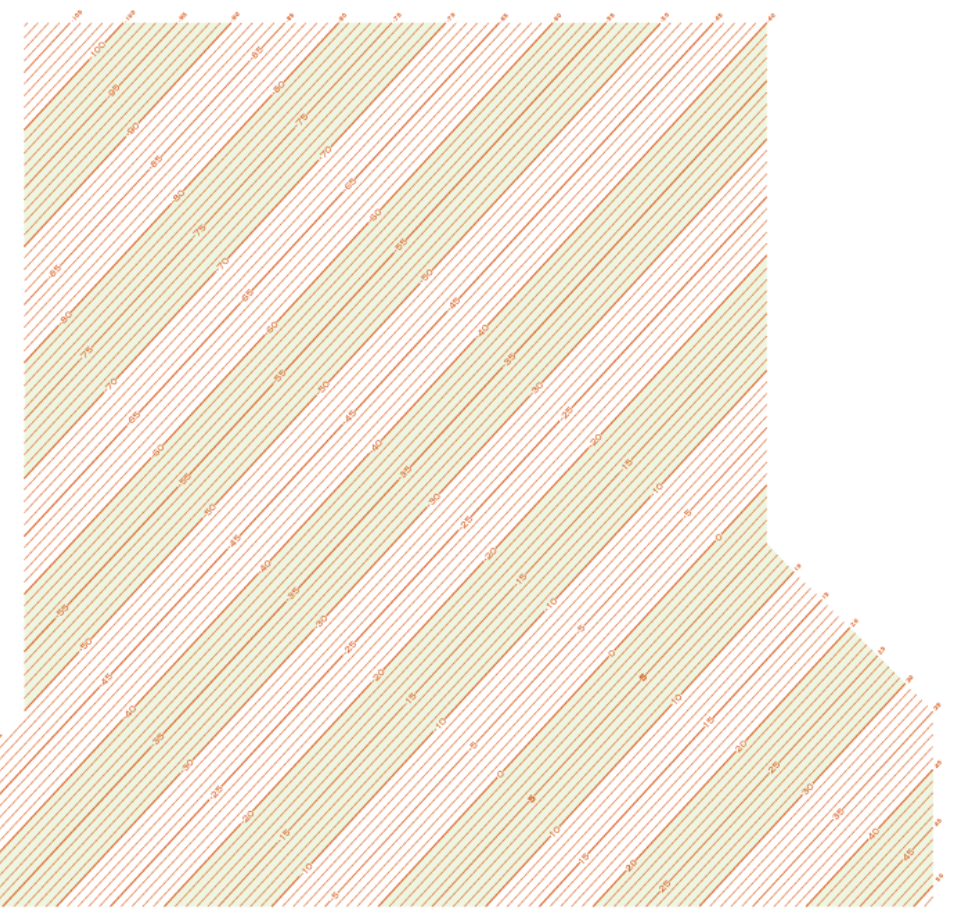
\includegraphics[width=\textwidth]{Figures/Iso-thermal-lines.png}
        \caption{Isothermal lines in Skew-T diagram}
    \end{minipage}
    \hfill
    \begin{minipage}[b]{0.48\textwidth}
        \centering
        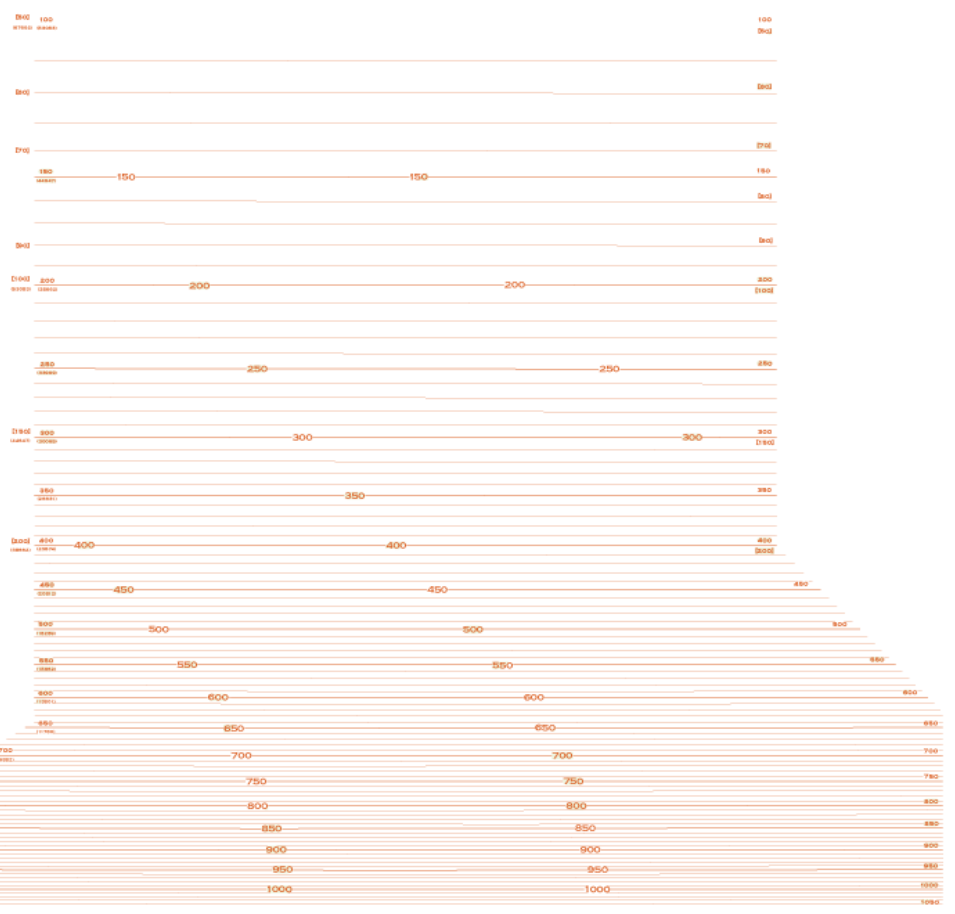
\includegraphics[width=\textwidth]{Figures/Iso-baric-lines.png}
        \caption{Isobaric lines in Skew-T diagram}
    \end{minipage}
\end{figure*}

\begin{figure*}[ht]
    \centering
    \begin{minipage}[b]{0.48\textwidth}
        \centering
        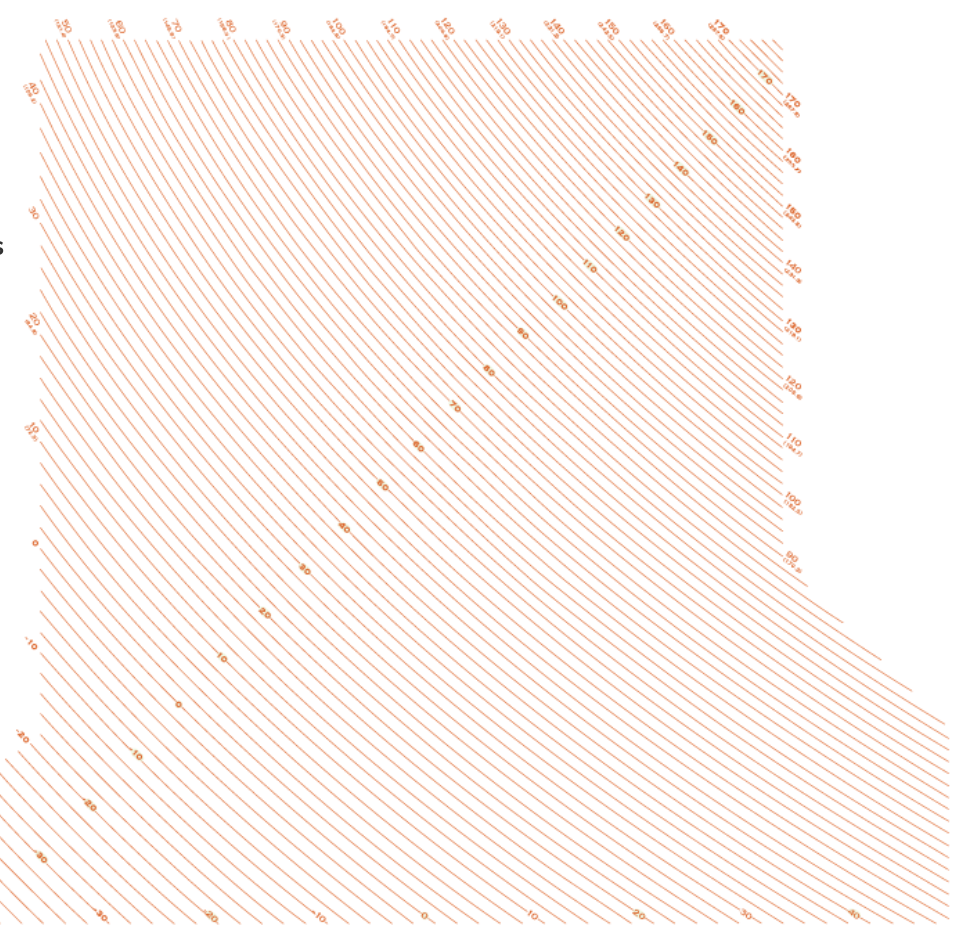
\includegraphics[width=\textwidth]{Figures/Dry-adiabat-lines.png}
        \caption{Dry-adiabat lines in Skew-T diagram}
    \end{minipage}
    \hfill
    \begin{minipage}[b]{0.48\textwidth}
        \centering
        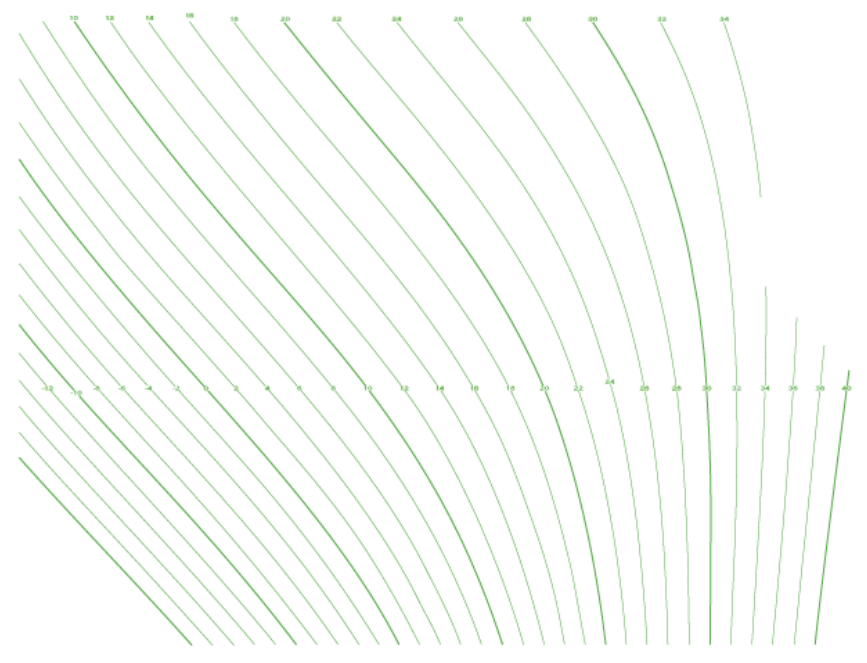
\includegraphics[width=\textwidth]{Figures/Moist-adiabat-lines.png}
        \caption{Moist-adiabat lines in Skew-T diagram}
    \end{minipage}
\end{figure*}

\begin{figure*}[ht]
    \centering
    \begin{minipage}[b]{0.48\textwidth}
        \centering
        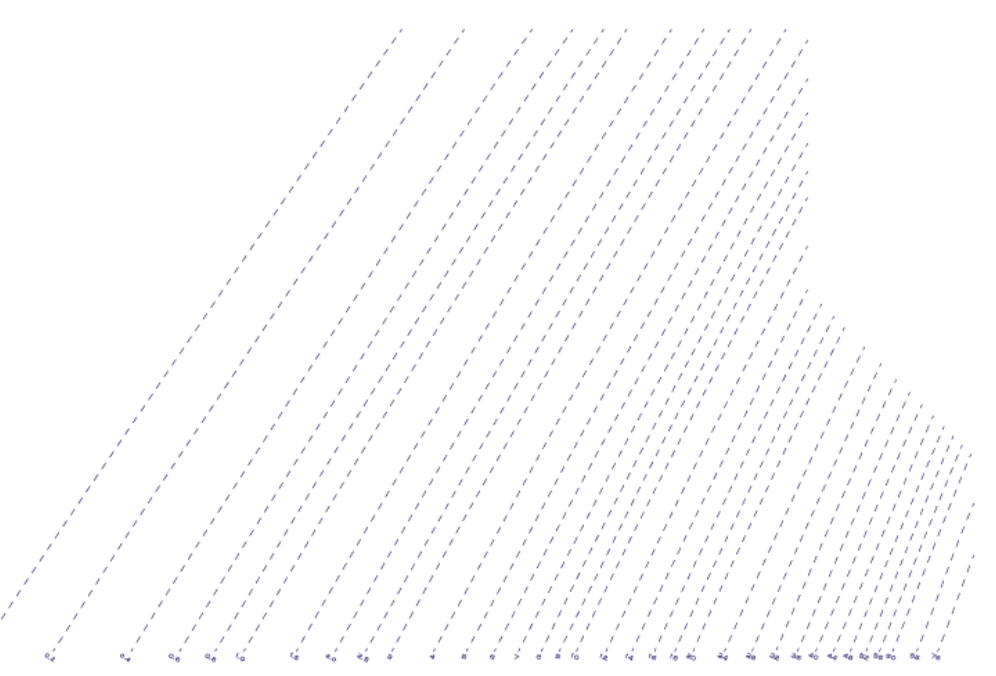
\includegraphics[width=\textwidth]{Figures/Mixing-ratio-lines.png}
        \caption{Mixing ratio lines in Skew-T diagram}
    \end{minipage}
\end{figure*}

\clearpage
\begin{figure*}[ht]\centering
	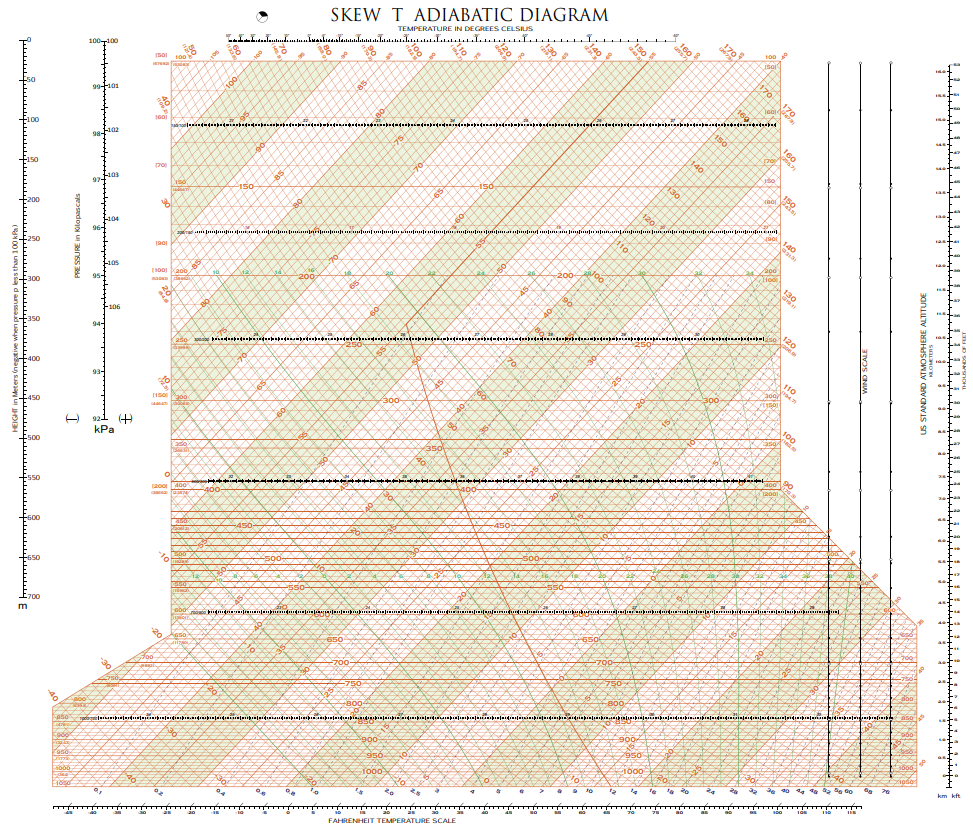
\includegraphics[width=\linewidth]{Figures/skew_t.png}
        \caption{Skew-T diagram}
        \label{fig:Skew-T_diagram}
\end{figure*}

% NOTE: COMPLETED L-14
% --------------------------------------------------------------------------------------
\clearpage

\section{Lecture 15 03/10/2024}

\subsection{. Cyclones}
\textbf{Properties of cyclones}
\begin{enumerate}[noitemsep]
    \item Centre of cylce is called Eye of cyclone.
    \item Cumulonimbus clouds forms the eye ball of cyclone.
    \item Maximum height to where it can reaches is Tropopause
\end{enumerate}

\begin{figure}[ht]
    \begin{center}
        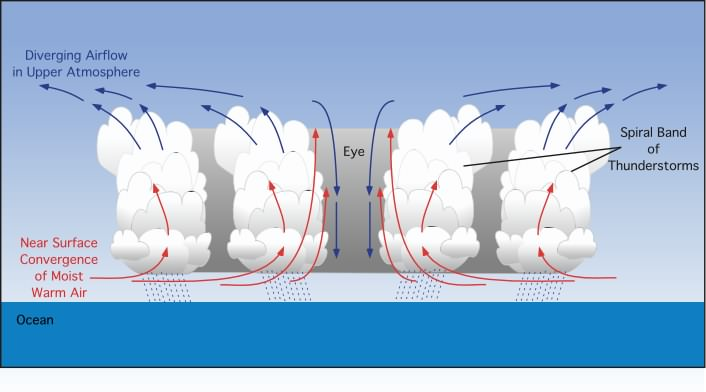
\includegraphics[width=0.45\textwidth]{Figures/hurricane_structure.jpg}
    \end{center}
    \caption{Internal Structure of cyclone}\label{fig:cyclone_structure}
\end{figure}
Image source: \myhref{https://web.mit.edu/~twcronin/Public/Lupit_Cross_Sections.html}{Internal Structure of cyclone}

\begin{figure}[ht]
    \begin{center}
        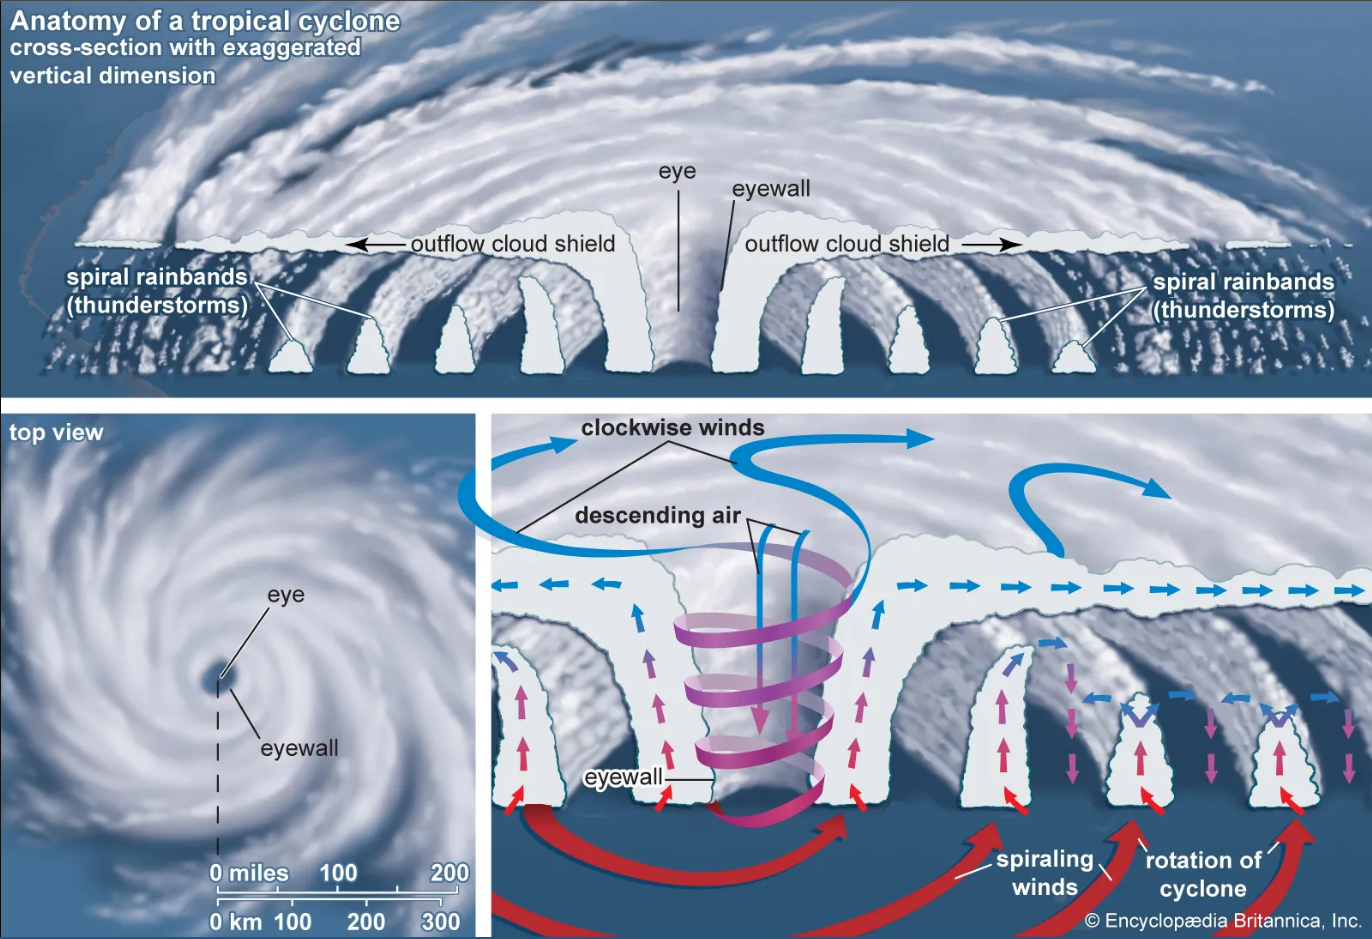
\includegraphics[width=0.45\textwidth]{Figures/cyclone_air_circulation.png}
    \end{center}
    \caption{ Air circulation in cyclone}\label{fig:cyclone_air_circulation}
\end{figure}
Image source: \myhref{https://www.britannica.com/science/tropical-cyclone}{ Air circulation in cyclone}

\subsection{. Specific enthaphy}
Enthaphy is heat content of state.
\begin{align}
    H        & = U + PV \\
    \Delta H & = \Delta U + \Delta (PV) \\
    \Delta H & = \Delta U + P \Delta V + V \Delta P \\
    \Delta H & = Q - W + P \Delta V + V \Delta P \\
    \Delta H & = Q - \cancel{P \Delta V} + \cancel{P \Delta V} + V \Delta P \\
    \Delta H & = Q + V \Delta P \\
    \text{ At const. Pressure} \\
    \Delta H & = Q \\
    h        & = u+ P \alpha \\
    dh       & = du + d(PV) \\
    dh       & = du + P d\alpha + \alpha dP \\
    dh       & = \delta q + \alpha dP \\
    \delta q &= dh - \alpha dP  \label{eq:enthalphy_heat}
    \text{ also,} \\
    \delta q &= C_p dT - \alpha dP  \label{eq:enthalphy_heat_1}
\end{align}
From Eq\myeqref{eq:enthalphy_heat} and Eq\myeqref{eq:enthalphy_heat_1}
\begin{align}
    dh - \alpha dP &= C_p -\alpha dP \\
    \text{ At const. Pressure} \\
    dh & = C_p dT
\end{align}
Enthalphy is "sensible heat" \\

\textbf{Conservative property}\\
For a hydrostatic atmosphere:
\begin{align}
    \frac{dp}{dz} = \rho g \Rightarrow dp = -\rho gdz \label{eq:hydrostaticeq}
\end{align}
Substitute Eq\myeqref{eq:enthalphy_heat_1} in Eq\myeqref{eq:hydrostaticeq}
\begin{align}
    \delta q &= C_p dT - \cancel{\alpha} \cancel{\rho} gdz \\
    \delta q &= C_p dT + gdz \\
    \delta q &= dh + d\phi \\
    \delta q &= d(h + \phi)
\end{align}
If process is adiabatic $\delta q=0$
\begin{align}
    h + \phi = \text{const} \label{eq:dry_static_equation}
\end{align}
Eq\myeqref{eq:dry_static_equation} called dry static equation.

This implies that when air parcel goes up (in geopotential) by the expense of heat content (enthalphy), i.e. [$h \uparrow \phi \downarrow$]. \\

\begin{center}
    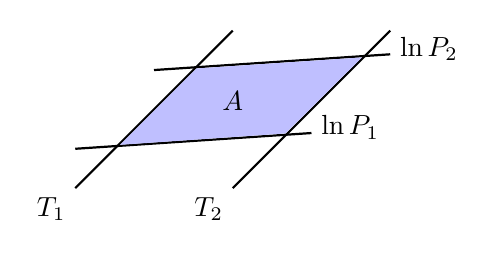
\begin{tikzpicture}
        % Draw the lines
        \draw[thick] (0, 0) -- (2, 2);       % Line 1
        \draw[thick] (0, 0.5) -- (3, 0.7);   % Line 2
        \draw[thick] (2, 0) -- (4, 2);       % Line 3
        \draw[thick] (1, 1.5) -- (4, 1.7);   % Line 4
        
        % Fill the area enclosed by the lines
        \begin{scope}
            \fill[blue!25] (0.57, 0.55) -- (2.67, 0.695) -- (3.64, 1.66) -- (1.54, 1.52) -- (0.57, 0.55);
        \end{scope}

        % Label the endpoints
        \node at (0, 0) [below left] {$T_1$};
        \node at (3, 0.5) [above right] {$\ln P_1$};
        \node at (2, 0) [below left] {$T_2$};
        \node at (4, 1.5) [above right] {$\ln P_2$};
        \node at (2, 1.1)  {$A$};
    \end{tikzpicture}
\end{center}

\begin{align}
    \text{Area } A &\propto (T_2-T_1)(\ln P_2 - \ln P_1) \\
                  &\propto (T_2-T_1)\ln \Big(\frac{P_2}{P_1}\Big)
\end{align}

\textbf{Cycle 1:}
\begin{align*}
    w_1 &= \int P d\alpha  \\
        &= P \int_{\alpha_1}^{\alpha_2} d\alpha \\
        &= P(\alpha_2 - \alpha_1) \\
        &= R_d(T_2-T_1)
\end{align*}

\textbf{Cycle 2:}
\begin{align*}
    w_2 &= \int P d\alpha  \\
        &= \int_{\alpha_1}^{\alpha_2} \frac{R_d T}{\alpha} d\alpha \\
        &= R_d T_2 \ln \Big(\frac{\alpha_2}{\alpha_1}\Big) \\
        &= R_d T_2 \ln \Big(\frac{P_1}{P_2}\Big)
\end{align*}

\textbf{Cycle 3:}
\begin{align*}
    w_3 &= \int P d\alpha  \\
        &= P \int_{\alpha_2}^{\alpha_1} d\alpha \\
        &= P(\alpha_1 - \alpha_2) \\
        &= R_d(T_1-T_2) \\
        &= - R_d(T_2-T_1)
\end{align*}

\textbf{Cycle 4:}
\begin{align*}
    w_4 &= \int P d\alpha  \\
        &= \int_{\alpha_2}^{\alpha_1} \frac{R_d T}{\alpha} d\alpha \\
        &= R_d T_1 \ln \Big(\frac{\alpha_1}{\alpha_2}\Big) \\
        &= R_d T_1 \ln \Big(\frac{P_2}{P_1}\Big) \\
        &= - R_d T_1 \ln \Big(\frac{P_1}{P_2}\Big)
\end{align*}

\begin{align*}
    w_{\text{net}} &= w_1 + w_2 + w_3 + w_4 \\
                   &= R_d(T_2-T_1) + R_d T_2 \ln \Big(\frac{P_1}{P_2}\Big) - R_d(T_2-T_1) - R_d T_1 \ln \Big(\frac{P_1}{P_2}\Big) \\
    \Rightarrow w_{\text{net}} &= 0
\end{align*}

% NOTE: COMPLETE L-15
% --------------------------------------------------------------------------------------
\clearpage

\section{Lecture 16 07/10/2024}

\subsection{. Lesson learnt from carnot cycle}
\begin{enumerate}[I]
    \item Thermodynamic effeciency of cyclone depends on sources, given by Eq\myeqref{eq:eff_carnot}

    When $T_1 =T_2$, carnot cycle does not exist called \textbf{Kelvin's Postulate}.

    Carnot engine is most effiecent at winter because of difference in termperature, casues diverse climate change.

    \item Transformation of heat is not possible from cold body to hot body called \textbf{Clausius postulate}

    \item Carnot cycle could give us definition for absolute zero temperature.

    \item All process are irreversible, however, slow process can be considered to be reversible.
\end{enumerate}

\subsection{. Entropy}
Let's recall that, 
\begin{align}
    q_1 &= R_dT_1\ln \Big(\frac{\alpha_2}{\alpha_1}\Big) \\
    \frac{q_1}{T_1} &= R_d\ln \Big(\frac{\alpha_2}{\alpha_1}\Big)
\end{align}

Similiarly,
\begin{align}
    q_2 &= -R_dT_2\ln \Big(\frac{\alpha_2}{\alpha_1}\Big) \\
    \frac{q_2}{T_2} &= R_d\ln \Big(\frac{\alpha_2}{\alpha_1}\Big) 
\end{align}

\begin{align}
    \frac{q_1}{T_1} + \frac{q_2}{T_2}=0, \label{eq:q1t1+q2t2} \quad \quad \quad q_1>0, q_2<0 
\end{align}

Efficency of heat engine:
\begin{align}
    \eta_{\text{rev}} = 1- \frac{T_2}{T_1} \\
    \eta_{\text{rev}} = \frac{T_1 - T_2}{T_1} \\
    T_1 \eta_{\text{rev}} = T_1 - T_2 \label{eq:eff_of_heat_engine}
\end{align}

Multiply and divide Eq\myeqref{eq:q1t1+q2t2} by $\eta_{\text{rev}}$ 
\begin{align}
    \frac{q_1}{T_1}\frac{\eta_\text{rev}}{\eta_\text{rev}} + \frac{q_2}{T_2}=0
\end{align}

From Eq\myeqref{eq:eff_of_heat_engine},
\begin{align}
    \frac{q_1}{T_1}\frac{\eta_\text{rev}}{(T_1-T_2)} + \frac{q_2}{T_2}=0
\end{align}
The above expression is applicable only if process is \textbf{perfectly reversible}.

If process is not prefrectly reversible, i.e., irreversible
\begin{align}
    \frac{q_1}{T_1}\frac{\eta_\text{irrev}}{(T_1-T_2)} + \frac{q_2}{T_2}<0
\end{align}

In general,
\begin{align}
    \sum_{i=1}^2 \frac{q_i}{T_i} & \leq 0,
    \begin{cases}
        = 0 & \text{if perfectly reversible}, \\
        < 0 & \text{if irreversible}
    \end{cases}\\
    \Rightarrow \sum_{i=1}^N \frac{q_i}{T_i} & \leq 0, \quad \text{for $N$ number of sources.}
\end{align}

If $N$ \rightarrow $\infty$ 
\begin{align}
    \underset{\substack{\text{cyclic}\\ \text{process}}}\oint \frac{\delta q}{T} \leq 0 \rightarrow \text{Entropy}
\end{align}

\begin{align}
    \delta q &= C_v dT +Pd\alpha \\
    \frac{\delta q}{T} &= C_v \frac{dT}{T} +P \frac{d\alpha}{T} \\
    \oint \frac{\delta q}{T} &= C_v \oint \frac{dT}{T} + \oint \frac{R T}{\alpha T} d\alpha \\
    ds = \oint \frac{\delta q}{T} &= C_v \oint \frac{dT}{T} + R \oint d\ln \alpha \\
    ds = \oint \frac{\delta q}{T} &= C_v \oint d\ln T + R \oint d\ln \alpha \\
    \Rightarrow ds = s_f - s_i &= \oint_i^f \frac{\delta q}{T} 
\end{align}

Number of states in which the system can have large disorder hence higher entropy.

(No. of molecule $\uparrow$) (No. of possible system states $\uparrow$) $\rightarrow$ (Entropy$\uparrow$)

\begin{question}[\label=16.1]{Show that entropy of ideal gas depends on intial and final state of temperature and volume.}
    \Rightarrow 
    ds = \oint \frac{dq}{T} = C_v \oint d(\ln T) + R \oint d(\ln \alpha) \\

    \Delta S = \int^f_i ds = S_f - S_i = C_v \ln \Big(\frac{T_f}{T_i}\Big) + R\ln\Big(\frac{\alpha_f}{\alpha_i}\Big) \\

    S_f = S_i + C_v \ln \Big(\frac{T_f}{T_i}\Big) + R\ln\Big(\frac{\alpha_f}{\alpha_i}\Big) \\

    S_f = S_i + C_v \ln \Big(\frac{T_f}{T_i}\Big) + C_v (\frac{R}{C_v})\ln\Big(\frac{\alpha_f}{\alpha_i}\Big) \\

    S_f = S_i + C_v \Big[ \ln\Big(\frac{T_f}{T_i}\Big) \times \Big(\frac{\alpha_f}{\alpha_i}\Big)^{\big(\frac{C_p-C_v}{C_v}\big)}\Big] \\

    S_f = S_i + C_v \Big[ \ln\Big(\frac{T_f}{T_i}\Big) \times \Big(\frac{\alpha_f}{\alpha_i}\Big)^{(\gamma - 1)}\Big] \text{where $\gamma= C_p/C_v$} 
\end{question}

% NOTE: COMPLETE L-16
% --------------------------------------------------------------------------------------
\clearpage

\section{Lecture 17 10/10/2024}

\subsection{. Entropy}
In last lecture we derived expression of entropy, i.e.
\begin{align*}
\oint \frac{q}{T} \leq 0 
\end{align*}

$\rightarrow$ Depends on the final and initial states of temperature and volume.

Let us consider a cyclic process with initial state $i$ and final state $f$, the path through which process occur be denoted by $R$ and $I$ representing reversible and irrreversible processes.
\begin{align*}
    i &\overset{R}{\longrightarrow} f \quad \text{Reversible} \\
    i &\overset{I}{\longrightarrow} f \quad \text{Irreversible}
\end{align*}

\begin{center}
    \begin{tikzpicture}
        % Place the points 1 and 2
        \draw (1,4) node[above left]{$i$};
        \draw (4,7) node[above right]{$f$};

        % Draw the almond shape using two arcs
        \draw[midar] (1,4) arc[start angle=180, end angle=90, x radius=3, y radius=3] 
            node[midway, above] {$I$};
        \draw[midar] (4,7) arc[start angle=360, end angle=270, x radius=3, y radius=3] 
            node[midway, below] {$R$};
    \end{tikzpicture}
\end{center}

As we know from any cyclic process
\begin{align}
    \oint \frac{q}{T} &\leq 0 \\
    \Big[\int^f_i \frac{q}{T}\Big]_R + \Big[\int^i_f \frac{q}{T}\Big]_I &\leq 0
\end{align}

Since, 
\begin{align}
    ds = \frac{\delta q}{T}
\end{align}
\begin{align}
    S_f - S_i + \Big[\int^i_f \frac{q}{T}\Big]_I &\leq 0 \\
    S_f - S_i &\geq \Big[\int^i_f \frac{q}{T}\Big]_I \\
    ds &\geq \Big[\int^i_f \frac{q}{T}\Big]_I \\
    Tds &\geq \delta q
\end{align}

It indicates that the upperbound of the heat abosorbedby the system during a given changes.

For an isolated system,
\begin{align}
    \delta q &= 0 \\
    S_f - S_i &\geq 0 \\ 
    S_f &\geq S_i 
\end{align}

For a spontaneous irreversible transformation, occuring in an isolated system, the final entropy is greater then initial entropy. 

\subsection{. 2$^{nd}$ law of themodynamics}
2$^{nd}$ law of themodynamics can be stated as:
\begin{enumerate}
    \item For reversible transformation, there is no change in entropy of universe.
    \item The entropy of universe increase as a result of irreversible transformation.
\end{enumerate}

\begin{align*}
    \Delta S_{\text{universe}} &= \Delta S_{\text{system}} +\Delta S_{\text{surrounding}} \\
    \Delta S_{\text{surrounding}} &= 0 \quad \text{For reversible transformation} \\
    \Delta S_{\text{surrounding}} &> 0 \quad \text{For irreversible transformation}
\end{align*}

% FIX: solve the question
\begin{question}[\label=17.1]{Calculate the change in air pressure if the specific entropy decrease by $0.05 Jg^{-1}K^{-1}$ and the ait temperature decrases by $5\%$.}
\Rightarrow  \text{To calculate the change in air pressure given the}

\text{specific entropy decrease and temperature change}

    \textbf{Given:}
    \begin{itemize}[noitemsep]
        \item Change in specific entropy: \( ds = -0.05 \, \mathrm{Jg^{-1}K^{-1}} \)
        \item Temperature decrease: \( dT = -0.05T \) (a decrease of \( 5\% \))
    \end{itemize}
\text{Assuming the process to be reversible} \\
    \textbf{Using the equation:}
    \begin{align*}
        ds &= C_p \, d\ln(T) - R \, d\ln(P)
    \end{align*}

    \textbf{Substituting values:}
    \begin{align*}
        dT &= -0.05T \Rightarrow d\ln(T) = \frac{dT}{T} = -0.05 \\
        ds &= C_p \, (-0.05) - R \, d\ln(P) \\
        -0.05 &= 1005 \, (-0.05) - 287 \, d\ln(P) \\
        -0.05 &= -50.25 - 287 \, d\ln(P) \\
        287 \, d\ln(P) &= -50.25 + 0.05 \\
        287 \, d\ln(P) &= -50.20 \\
        d\ln(P) &= \frac{-50.20}{287} \approx -0.174
    \end{align*}

    \textbf{Integrating:}
    \[
    P_f = P_i e^{-0.174}
    \]
    where \( P_f \) is the final pressure and \( P_i \) is the initial pressure.   ds &= C_p d\ln(T) - R d\ln(P)
\end{question}

Recall that,
\begin{align}
    \theta &= T\Big(\frac{1000}{P}\Big)^{\frac{R_d}{C_p}} \\
    \ln \theta &= \ln T + \frac{R_d}{C_p}\ln(1000) - \frac{R_d}{C_p}\ln P \\ 
    C_p d(\ln \theta) &= C_p d(\ln T) - R_d d(\ln P) \label{eq:2ndLaw1}
\end{align}

From 1$^{st}$ law of thermodynamic,
\begin{align}
    \delta q &= C_p dT - \alpha dP \\
    ds &= \frac{C_p dT}{T} - \frac{\alpha dP}{T} \\
    ds &= \frac{C_p dT}{T} - \frac{R_d dP}{P} \\
    ds &= C_p d\ln(T) - R d\ln(P) \label{eq:2ndLaw2}
\end{align}

Comparing Eq\myeqref{eq:2ndLaw1} and Eq\myeqref{eq:2ndLaw1} we can find that,
\begin{align}
    ds &= C_pd(\ln \theta) \\
    S &= C_p \ln \theta + \text{const.} 
\end{align}

Therefore, lines of constant potential temperature are lines of constant entropy, but not if process becomes irreversible.
Specific entropy is given by logarithm of potential temperature, when $\theta$ remains constant $\implies$ entropy remains constant.\\
For irreversible transformation $$ds >0 \quad d\theta=0$$

All isentropic process are adiabatic but all adiabatic process are not isentropic.

\newpage

\begin{question}[\label=17.1]{During a process a parcel of dry air decent from 900 to 950$hPa$ and if specific entropy decreases by 30$Jkg^{-1}K^{-1}$. If it's initial temperature is 273$K$; What is it's final temperature and potential temperature?}
\Rightarrow \text{The relationship between specific entropy S,} \\ \text{temperature T, and pressure P for an ideal gas assuming} \\ \text{the process to be reversible can be expressed as:}

    \begin{align*}
        ds &= C_p \, d\ln(T) - R \, d\ln(P)
    \end{align*}

    \textbf{Given:}
    \begin{align*}
        P_i&=900hPa, \\
        P_f&=950hPa, \\
        T_i&=273K,
    \end{align*}
    \textbf{Substituting values:}
    \begin{align*}
        -30&=1005 \ln\Big(\frac{T_f}{273}\Big) - 287 \ln\Big(\frac{950}{900}\Big) \\
        -14.4827&=1005 \ln\Big(\frac{T_f}{273}\Big) \\
        T_f&=273 \times e^{-0.0144} \\
        T_f&=269.094K
    \end{align*}
    \textbf{Potential Temperature:}
    \begin{align*}
        \theta &= T_f \left(\frac{P_0}{P_f}\right)^{R/C_p}
    \end{align*}
    \text{Substituting the values:}
    \begin{align*}
        \theta = 269.7 \times \Big(\frac{950}{900}\Big)^{0.2855} \approx 273.6K
    \end{align*}

\therefore \text{The final temperature is 269$K$ and potential}\\ \text{temperature is 273.6$K$}
\end{question}

% NOTE: COMPLETE L-17
% --------------------------------------------------------------------------------------
\clearpage

\section{Lecture 18 10/10/2024}
\subsection{. Special Forms of 2$^{rd}$ law of Thermodynamics}

\begin{enumerate}
    \item For finite isothermal transformation
            \begin{align}
                \Delta U &= 0 \\
                \Delta S &\geq \int \frac{\delta q}{T} \\
                \Delta S &\geq \frac{1}{T} \int \delta q \\
                \Delta S &\geq \frac{q}{T} \\
                \Delta S &\geq \frac{w}{T}
            \end{align}

    \item For adiabatic transformation
            \begin{align}
                \Delta S &\geq 0
            \end{align}

    \item For Isochoric transformation
            \begin{align}
                \Delta S &\geq C_v \frac{d T}{T} \\
                \Delta S &\geq C_v \ln\Big(\frac{T_f}{T_i}\Big)
            \end{align}

    \item For Isobaric transformation
            \begin{align}
                \Delta S &\geq C_p \frac{d T}{T} \\
                \Delta S &\geq C_p \ln\Big(\frac{T_f}{T_i}\Big)
            \end{align}

    \item Combination of 1$^{st}$ and 2$^{nd}$ law
        \begin{align}
            \delta q &= C_p dT - \alpha dp \\
            ds &\geq \frac{q}{T} \\
            Tds &\geq C_p dT - \alpha dp \\
            Tds &\geq dh - \alpha dp \\
        \end{align}
        similiarlly,
        \begin{align}
            \delta q &= C_v dT - \alpha dp \\
            ds &\geq \frac{q}{T} \\
            Tds &\geq C_v dT - \alpha dp \\
            Tds &\geq du - \alpha dp
        \end{align}
\end{enumerate}

\subsection{. Moist Processes}
There are three processes in moist gases:
\begin{itemize}[noitemsep]
    \item Saturation
    \item Sub-saturation
    \item Supersaturation
\end{itemize}

\textbf{Evaporation:} Some water molecules have sufficient kinetic energy to break free from the intermolecular forces of attraction.

\textbf{Condensation:} When water vapor cools down, molecules lose kinetic energy and form liquid droplets due to intermolecular attractions.

\begin{figure}[h!]
    \centering
    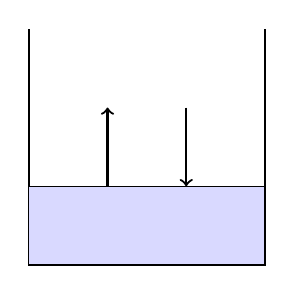
\begin{tikzpicture}
        % Draw the container using three solid lines
        \draw[thick] (0,0) -- (0,3); % left line of the container
        \draw[thick] (3,0) -- (3,3); % right line of the container
        \draw[thick] (0,0) -- (3,0); % bottom line of the container

        \draw[fill=blue!15] (0,0) rectangle (3,1); % square representing the object

        \draw[->][thick] (1, 1) -- (1, 2); % upward arrow (evaporation)
        \draw[->][thick] (2, 2) -- (2, 1); % downward arrow (condensation)
    \end{tikzpicture}
    \caption{Saturated state}
\end{figure}

\begin{figure}[h!]
    \centering
    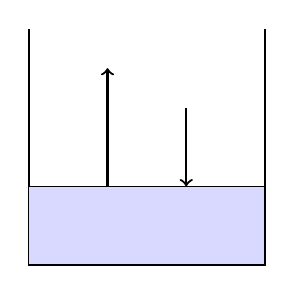
\begin{tikzpicture}
        % Draw the container using three solid lines
        \draw[thick] (0,0) -- (0,3); % left line of the container
        \draw[thick] (3,0) -- (3,3); % right line of the container
        \draw[thick] (0,0) -- (3,0); % bottom line of the container

        \draw[fill=blue!15] (0,0) rectangle (3,1); % square representing the object

        \draw[->][thick] (1, 1) -- (1, 2.5); % upward arrow (evaporation)
        \draw[->][thick] (2, 2) -- (2, 1); % downward arrow (condensation)
    \end{tikzpicture}
    \caption{Sub-Saturated state}
\end{figure}

\begin{figure}[h!]
    \centering
    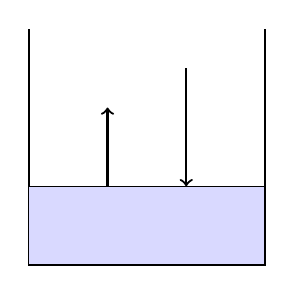
\begin{tikzpicture}
        % Draw the container using three solid lines
        \draw[thick] (0,0) -- (0,3); % left line of the container
        \draw[thick] (3,0) -- (3,3); % right line of the container
        \draw[thick] (0,0) -- (3,0); % bottom line of the container

        \draw[fill=blue!15] (0,0) rectangle (3,1); % square representing the object

        \draw[->][thick] (1, 1) -- (1, 2); % upward arrow (evaporation)
        \draw[->][thick](2, 2.5) -- (2, 1); % downward arrow (condensation)
    \end{tikzpicture}
    \caption{Super-Saturated state}
\end{figure}
For saturated state rate of evaporation is equals to rate of condensation.

\textbf{Saturation vapor pressure($e_s$)} depends only on temperature.

\begin{figure}[htb!]
    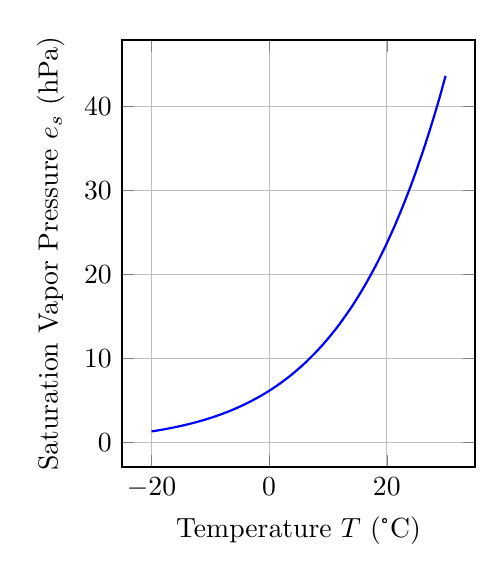
\begin{tikzpicture}
        \begin{axis}[
            width=0.5*\textwidth, height=7cm,
            xlabel={Temperature $T$ (°C)},
            ylabel={Saturation Vapor Pressure $e_s$ (hPa)},
            grid=major,
            domain=-20:30,
            samples=100,
            thick
        ]
        % Clausius-Clapeyron equation parameters
        \addplot [
            blue,
            domain=-20:30,
        ] 
        {6.11 * exp((2.5e6 / 461) * (1 / 273.15 - 1 / (x + 273.15)))};
        \end{axis}
    \end{tikzpicture}
    \caption{Saturation Vapor Pressure $e_s$ vs Temperature $T$}
\end{figure}

\textbf{Boiling Point:} The temperature at which vapor pressure is equal to atmospheric temperature at the pressure of $1013 hPa$.

\subsection{. Relative humidity}
Relative humidity is defined as ratio of vapor pressure to saturation vapor pressure.
\begin{align}
    \text{Relative humidity (RH)} = \frac{e}{e_s} \times 100\%
\end{align}
\begin{align}
    e &< e_s(T) \rightarrow \text{Sub-Saturation} \\
    e &= e_s(T) \rightarrow \text{Saturation} \\
    e &> e_s(T) \rightarrow \text{Super-Saturation}
\end{align}

\textbf{\textit{Note:} Specific humidity is associated with mass}

\subsection{. Dew point temperature}
There are 2 ways to make sub-saturated to saturated:
\begin{enumerate}[noitemsep]
    \item Reduce temperature
    \item Add moisture, so that vapor pressure increase.
\end{enumerate}

If moisture amount remains constant and temperature is reduced, thus saturation is achieved and this temperature is called \textbf{Dew point temperature}.

\subsection{. Latent heat}
Total energy required to convert unit mass from one phase to another.

Specific enthapy of phase change.

Latent heat of water at STP is $\approx 10^6 J/Kg$ (Depends on temperature)

\subsubsection*{Latent heat of evaporation}
Latent heat of evaporaton of water at:
\begin{itemize}[noitemsep]
    \item $T=-40^\circ C$, \quad Latent heat $=2.6 \times 10^6J/Kg$ 
    \item $T=0^\circ C$, \quad Latent heat $=2.5 \times 10^6J/Kg$ 
    \item $T=40^\circ C$, \quad Latent heat $=2.26 \times 10^6J/Kg$ 
\end{itemize} 

\subsubsection*{Latent heat of fusion}
Latent heat of fusion of water at STP $=3.3 \times 10^6 J/Kg$

\subsubsection*{Latent heat of sublimation}
Latent heat of sublimation of water at STP $=2.83 \times 10^6 J/Kg$

\begin{question}[\lable=18.1]{On a winter day the ouside air have temperature of -15$^\circ$C and relative humidity of $70\%$.\newline
    a. If the outside air is brought inside and heated to room temperature of 20$^\circ$C without adding moisture. What is new relative humidity?\newline
    b. If the room volume is 60m$^3$ then what mass of water must be added to the air by the humidifier to raise the relative humidity to 40\%?\newline
    c. How heating is needed to accomplish a. and b.?
    }
    \Rightarrow
        \Rightarrow a. \text{The saturation vapor pressure at -15$^\circ$C can be} \\ \text{found using} \text{lookup tables.}\\ \text{For $T=$ −15$^\circ$C, the saturation vapor pressure,}

            $$e_s(-15^\circ C) \approx 1.93 hPa$$
        \text{Given the relative humidity is 70\%, the actual vapor} \\ \text{pressure at −15$^\circ$C is:}

            $$e =\frac{70}{100}\times 1.93 hPa \approx 1.35hPa$$
        \text{For $T=$ 20$^\circ$C, the saturation vapor pressure,}
            $$e_s(20^\circ C) \approx 23.37 hPa$$
        \text{Using the actual vapor pressure calculated earlier} \\ \text{$e=1.35$hPa and the new saturation vapor pressure} \\ \text{$e_s(20^\circ C)$}:
        $$RH at 20^\circ C = \frac{e}{e_s} \times 100\% = \Big(\frac{1.35 hPa}{23.37hPa}\Big) \times 100\% \approx 5.8\%$$

        \Rightarrow b. \text{To find mass of water needed to raise RH to 40\%}

        $$e= \frac{40}{100} \times 23.37hPa = 9.35hPa$$
        \text{The amount of water vapor needed to raise the humidity} \\ \text{is proportional to the difference in vapor pressure:}
            $$\Delta e=9.35hPa - 1.35hPa = 8.00hPa$$
        \text{The mass of water vapor can be calculated using the}\\ \text{ideal gas law:}
            $$m= \frac{\Delta eV}{R_v T}$$
            $$m= \frac{800Pa \times 60 m^3}{461.5Jkg^{-1} K^{-1} \times 293K} \approx 0.35kg$$

    \Rightarrow c. \text{Heating Needed to Accomplish (a) and (b)}

    \begin{align*}
        m_{\text{air}} &= \frac{95000 \, \mathrm{Pa} \times 60 \, \mathrm{m^3}}{287 \, \mathrm{Jkg^{-1}K^{-1}} \times 258 \, \mathrm{K}} \approx 77.7 \, \mathrm{kg} \\
        Q_{\text{air}} &= 77.7 \times 1005 \times 35 \approx 2.73 \times 10^6 J \\
        Q_{\text{water}} &= 0.35 \times 2.5 \times 10^6 = 0.875 \times 10^6 J\\
        Q_{\text{total}} &= 2.73 \times 10^6 + 0.875 \times 10^6 \approx 3.61 \times 10^6 J
    \end{align*}
\end{question}

% WARN: INCOMPLETE L-18 que.
% NOTE: COMPLETE L-18
% --------------------------------------------------------------------------------------
\clearpage

\section{Leture 19 21/10/2024}
\subsection{The Clausius-Clapeyron equation}
Let $L$ is latent heat associated with phase change of a liquid($i$) to vapor($f$) state:
\begin{align}
    L &= \int dq \\
    L &= \int^f_i du + \int^f_i Pd\alpha \\
    L &= u_f - u_i + e_s(\alpha_f - \alpha_i) \label{eq:latent_heat_1}
\end{align}
where $e_s \rightarrow$ saturation vapor pressure

When phase cahnge happen, temperature remains constant, therefore
\begin{align} 
    L &= T\int \frac{\delta q}{T} \\
    L &= T \int^f_i ds \\
    L &= T (S_f -S_i) \label{eq:latent_heat_2}
\end{align}

From Eq\myeqref{eq:latent_heat_1} and Eq\myeqref{eq:latent_heat_2}
\begin{align}
    T(S_f-S_i) &= U_f-U_i + e_s(\alpha_f - \alpha_i) \\
    TS_f - U_f - e_s\alpha_f &= TS_i - U_i - e_s\alpha_i \\
    U + e_s\alpha - TS &= \text{Const.} = G
\end{align}
where $G$ is Gibbs energy

However, Gibbs energy is not constant when pressure and temperature changes.
\begin{align}
    dG &= du + e_s d\alpha + \alpha de_s - Tds - sdT \\
    dG &= \cancel{Tds} + \alpha de_s - \cancel{Tds} -sdT \\
    dG &= \alpha de_s - sdT
\end{align}

consider a situation when liquid phase and vapor phase are in equilibrium 
\begin{align}
    dG_1 &=dG_2 \\
    \alpha_i de_s - S_idT &= \alpha_f de_s - S_fdT \\
    \frac{S_f - S_i}{\alpha_f - \alpha_i} &= \frac{de_s}{dT}\\
    \frac{L}{T(\alpha_f-\alpha_i)} &= \frac{de_s}{dT} \label{eq:clasuius-clapeyron}
\end{align}
Eq \myeqref{eq:clasuius-clapeyron} is called Clasuius-Clapeyron equation.

Let initial state($i$) be liquid state and final state($f$) be vapor state (evaporation)
\begin{align}
    \frac{e_s}{dT} &= \frac{L}{T(\alpha_v - \alpha_l)}
\end{align}
For atmosphere $\alpha_v \ll \alpha_l$. therefore,
\begin{align}
    \frac{e_s}{dT} &\approx \frac{L}{T\alpha_v}
\end{align}
Using ideal gas equation $e_s\alpha_v = R_vT$,
\begin{align}
    \frac{de_s}{dT} &= \frac{Le_s}{R_vT^2} \label{eq:clasuius-clapeyron_0}
\end{align}

Integrate form of Clausius-Clapeyron equation:
\begin{align}
    \int^{e_s}_{e_0}\frac{e_s}{e_s} &= \int^{T}_{T_0}\frac{LdT}{R_vT^2} \\
    \ln\frac{e_s}{e_0} &= \frac{L}{R_v} \Big[\frac{1}{T_0} - \frac{1}{T}\Big] \\
    e_s &= e_0\exp\Big(\frac{L}{R_v} \Big[\frac{1}{T_0} - \frac{1}{T}\Big]\Big)
\end{align}

Standard values $T_0 = 273$ K, $e_0=611$ Pa or $6.11$ hPa,

$L= 2.5 \times 10^6$ J/kg, $R_v=461$ JK$^{-1}$kg

$e_s(T)\approx Ae^{-B/T}$, where $A=2.53\times10^{11}$Pa, $B=5420$K.

This gives more accurate equation for temperature range from $-30^\circ$C \leqslant T \leqslant $35^\circ$C
\begin{align}
    e_s(T) = 611.2\Big[\frac{17.69T_c}{T_c_243.5}\Big]
\end{align}
where $T_c$ is temperature in celcius scale

For Ice,
\begin{align}
    e_i(T) &= e_{i0}\exp\Big(\frac{L_s}{R_v} \Big[\frac{1}{T_0} - \frac{1}{T}\Big]\Big)
\end{align}
where $T_c$ is temperature in celcius scale and $L_s$ is latent heat of sublimation.

$e_s(T)\approx A_ie^{-B_i/T}$, where $A=3.41\times10^{12}$Pa, $B=6130$K.

\begin{question}[\labe:19.1]{For T of $265$K; find the value of $e_i$ and $e_s$.}
    \Rightarrow e_i(T) &= 611.2 \times 10^{12} \times e^{-\frac{6130}{265}} \\
                       &= 3060.65 Pa

    \Rightarrow e_s(T) &= 2.53 \times 10^{11} \times e^{-\frac{5420}{265}} \\
                       &= 331.56 Pa
\end{question}

$e_i < e_s \rightarrow$ at subfreezing temperatures, the environment that is saturated w.r.t liquid water is supersaturated w.r.t ice.

% NOTE: COMPLETE L-19
% --------------------------------------------------------------------------------------
\clearpage

\section{Lecture 20 23/10/2024}
\subsection{Saturation mixing ratio}

\textbf{Mixing ratio:}
\begin{align}
    \omega &= \frac{m_v}{m_d} \\
    \omega &= \frac{\rho_v}{\rho_d}
\end{align}

\begin{align}
    \omega &= \frac{\epsilon e}{P - e} \\
    \omega &\approx \frac{\epsilon e}{P}
\end{align}
where $e=\frac{R_d}{R_v}=$ 0.622 \\
\newline
\textbf{Saturation mixing ratio:}
\begin{align}
    \omega_s(T,P) &\approx \frac{\epsilon e_s(T)}{P} \quad \text{Unit: g/kg} \\
    \omega_s(T,P=622\text{hPa}) &\approx \frac{0.622 e_s(T)}{622} = 0.001 \; \text{kg/kg} \\
    \omega_s(T,P=622\text{hPa}) &\approx 0.001 \; \text{kg/kg} \\
    \omega_s(T,P=622\text{hPa}) &\approx e_s(T) \; \text{g/kg} 
\end{align}

\begin{question}[\label:20.1]{Using skew-T diagram determine the saturation vapor pressure at -10$^\circ$C.}
    \Rightarrow $e_s=$2.75hPa
\end{question}
\begin{figure}[!ht]
    \centering
    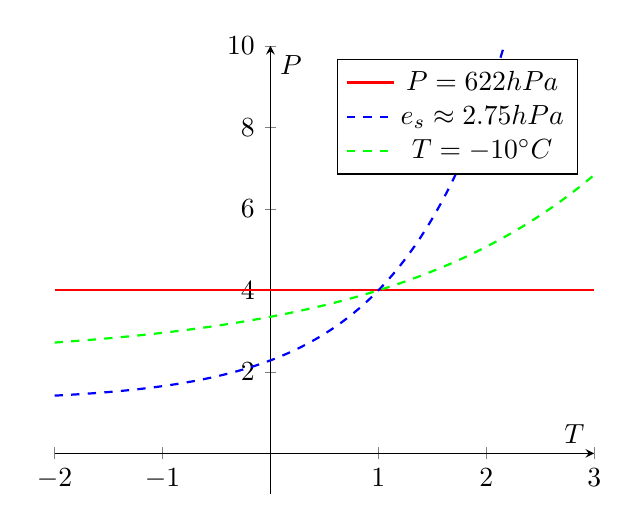
\begin{tikzpicture}
        \begin{axis}[
            axis lines=middle,
            xlabel=$T$, ylabel=$P$,
            domain=-2:3,
            samples=100,
            xmin=-2, xmax=3, ymin=-1, ymax=10,
            legend pos=north east
        ]

        % Horizontal line at y = 4
        \addplot[red, thick] {4};
        \addlegendentry{$P = 622hPa$}

        % Exponential functions
        \addplot[blue, thick, dashed] {exp(x) - exp(1) + 4};
        \addlegendentry{$e_s \approx 2.75hPa$}

        \addplot[green, thick, dashed] {exp(0.5*x) - exp(0.5) + 4};
        \addlegendentry{$T = -10^\circ C$}
        \end{axis}
    \end{tikzpicture}
\end{figure}

\begin{question}[\label:20.2]{Using Skew-T diagram determine the relative humidity of air parcel having temperature 20$^\circ$C and dew point  Temperature of 10$^\circ$C at presssure 850hPa}
    \Rightarrow \omega_s(20$^\circ$C,850\;hPa) = 18\;hPa \\
    \omega_s= \frac{\epsilon e_s(T)}{P} \\
    \frac{\omega}{\omega_s} \approx \frac{e}{e_s(T)}\\
    RH = \frac{e}{e_s(T)}\times 100 \% \\
    RH = \frac{\omega}{\omega_s}\times 100 \% \\
    RH = \frac{9}{18}\times 100 \% \\
    RH = 50\%
\end{question}

% NOTE: COMPLETE L-20
% --------------------------------------------------------------------------------------
\clearpage

\section{Lecture 21 24/102024}
\subsection{Lifting Conduction Level (LCL)}
\begin{align*}
    \omega_s &= \frac{\epsilon e_s(T)}{P}
\end{align*}

As $P$ decrease $T$ decrease.

$\frac{d\omega_s}{dp}$ decides how saturation vapor pressuredepends on pressure only (not on both Temperature and Pressure)

\begin{align}
    \frac{d\omega_s}{dP} &= \frac{d}{dP}\Big[\frac{\epsilon e_s(T)}{P}\Big] \\
                         &= \epsilon\Big[\frac{1}{P}\frac{de_s(T)}{dP}-\frac{e_s}{P^2}\Big] \\
                         &= \frac{\epsilon e_s}{P}\Big[\frac{1}{e_s}\frac{de_s(T)}{dP}-\frac{1}{P}\Big] \\
                         &= \frac{\epsilon e_s}{P}\Big[\frac{1}{e_s}\frac{de_s(T)}{dT}\frac{dT}{dP}-\frac{1}{P}\Big]
\end{align}
Using Clausius-Clapeyron equation Eq\myeqref{eq:clasuius-clapeyron_0}
\begin{align}
    \frac{d\omega_s}{dP} &= \frac{\epsilon e_s}{P}\Big[\frac{1}{\cancel{e_s}}\frac{L\cancel{e_s}}{R_vT^2}\frac{dT}{dP}-\frac{1}{P}\Big] \\
    \frac{d\omega_s}{dP} &= \frac{\epsilon e_s}{P}\Big[\frac{L}{R_vT^2}\frac{dT}{dP}-\frac{1}{P}\Big] \label{eq:dwdp}
\end{align}
Since process is adiabatic (Lifting of moist air):
\begin{align}
    C_p dT-\alpha dP &= 0 \\
    C_p \frac{dT}{dP}-\alpha &= 0 \\
    \frac{dT}{dP} &= \frac{\alpha}{C_p} \\
    \frac{dT}{dP} &=\frac{R_dT}{C_pP} \label{eq:dTdP}
\end{align}
Substiting Eq\myeqref{eq:dTdP} in Eq\myeqref{eq:dwdp}, we get
\begin{align}
    \frac{d\omega_s}{dP} &= \frac{\epsilon e_s}{P}\Big[\frac{L}{R_vT^2}\frac{\alpha}{C_p}-\frac{1}{P}\Big] \\
    \frac{d\omega_s}{dP} &= \frac{\epsilon e_s}{P}\Big[\frac{L}{R_vT^{\cancel{2}}}\frac{R_d\cancel{T}}{C_pP}-\frac{1}{P}\Big] \\
    \frac{d\omega_s}{dP} &= \frac{\epsilon e_s}{P^2}\Big[\frac{L}{R_vT}\frac{R_d}{C_p}-1\Big] \\
    \frac{d\omega_s}{dP} &= \frac{\omega_s}{P}\Big[\frac{R_dL}{R_vC_pT}-1\Big] \\
    \frac{d\omega_s}{dP} &= \frac{\omega_s}{P}\Big[\frac{\epsilon L}{C_pT}-1\Big]
\end{align}

$\omega_s$ decreases w.r.t height (Since $P$ decrease with height). $\omega_s$ decreases for any adiabatic uplift of air parcel.

Lifting Conduction Level is at $\omega =\omega_s$ 

Lifting Conduction Level is a level at which cloud start forming. It could be either Presure level or Temperature level).

\begin{question}[\label=21.1]{Find out LCL for an air parcel which has a temperature of 30$^\circ$C and dew point temperature of 0$^\circ$C at 1000hPa.}
    \Rightarrow 650hPa
\end{question}

\begin{question}[\label=21.2]{Find out LCL for an air parcel which has a temperature of 25$^\circ$C and dew point temperature of 18$^\circ$C at 900hPa.}
    \Rightarrow 920hPa
\end{question}

\begin{align}
    \text{LCL(Km)} &\approx \frac{T-T_0}{8} \\
    \text{LCL(hPa)} &= p \exp(-0.044\Delta T_d)
\end{align}
where $\Delta T_d$ is dew point depression which is eequal to $(T-T_d)$.

Just above LCL $\rightarrow$ phase change happen $\rightarrow$ release of latent heat which provides extra amount of energy, therefore, parcel will no longer follow dry adibat , but \textbf{moist adiabatic lapse rate}. It depends upon moisture content present in air.

This process is called \textbf{pseudo-adiabatic process} because mass get lost in precipitation. \newline

Dry adiabat lapse rate (DALR):
\begin{align*}
    \Gamma_d = \frac{g}{c_p}= 9.8^\circ C/km
\end{align*}
Above LCL, parcel will follow \textbf{saturated adiabatic lapse rate $\Gamma_s$} which is always less than dry adiabatic lapse rate, i.e. ($\Gamma_s < \Gamma_d$)

% NOTE: COMPLETE L-21
% --------------------------------------------------------------------------------------
\clearpage

\section{Leture 22 25/10/2024}
\subsection{. Saturation Adiabatic Lapse Rate }
\begin{align}
    \delta q &= C_p dT - \alpha dP
\end{align}

$\delta q =0$ since process is adiabatic for dry adiabat $\Gamma_d$, but for aturation adiabatic ($\Gamma_s$) $\delta q \neq 0$

Additon of heat from latent heat of water vapor 
\begin{align}
    \delta q &= -Ld\omega_s
\end{align}
where $\omega_s$ is saturation mixing ratio.

Therefore,
\begin{align}
    -Ld\omega_s &= C_pdT - \alpha dP
\end{align}

The term $\omega_s$ changes w.r.t pressure and temperature,
\begin{align}
    d\omega_s = \frac{\patial \omega_s}{\partial P} dP +  \frac{\patial \omega_s}{\partial T} dT
\end{align}

Using the expression $\omega_s \approx \frac{\epsilon e_s}{P}$
\begin{align}
    d\omega_s &= -\frac{\epsilon e_s}{P^2} dP + \frac{\epsilon e_s}{P} \frac{1}{e_s}\frac{de_s}{dT}dT \\
    d\omega_s &= -\omega_s \frac{dP}{P} + \omega_s \frac{L}{R_v T^2}dT \\
    -Ld\omega_s &= L\omega_s\frac{dP}{P} - \omega_s \frac{L^2}{R_v T^2}dT \\
    c_pdT - \alpha dP &= L\omega_s \frac{dP}{P} - \frac{L^2\omega_s}{R_vT^2}dT
\end{align}

Invoking hydrostatic approximation
\begin{align}
    \frac{\partial P}{\partial z} &= -\rho g \\
    gdz &= -\alpha dP
\end{align}
\begin{align}
    \frac{c_pdT}{gdz} - \frac{\alpha dP}{-\alpha dP} &= \frac{L\omega_s \frac{dP}{P}}{-\alpha dP} - \frac{\frac{L^2\omega_s}{R_vT^2}dT}{gdz} \\
    \frac{c_pdT}{gdz} - \frac{\cancel{\alpha dP}}{-\cancel{\alpha dP}} &= \frac{L\omega_s \frac{\cancel{dP}}{P}}{-\alpha \cancel{dP}} - \frac{\frac{L^2\omega_s}{R_vT^2}dT}{gdz} \\
    \frac{c_pdT}{gdz} + 1 &= \frac{L\omega_s}{-\alpha P} - \frac{L^2\omega_sdT}{R_v T^2 gdz}\\
    \Big(\frac{L^2\omega_s}{R_v g T^2} + \frac{c_p}{g}\Big)\frac{dT}{dz} &= \frac{L\omega_s}{\alpha P} +1 \label{eq:lapse_rate}
\end{align}

Recall $\Gamma_d=\frac{g}{c_p}\frac{T'}{T} \approx \frac{g}{c_p}$

where $T'$ is temperature of parcel and $T$ is temperature of atmosphere.

Multipling $\frac{g}{c_p}$ to Eq\myeqref{eq:lapse_rate}
\begin{align}
    \Big(\frac{L^2\omega_s}{R_v g T^2}\frac{g}{c_p} + \frac{c_p}{g}\frac{g}{c_p} \Big)\frac{dT}{dz} &= \frac{L\omega_s}{\alpha P}\frac{g}{c_p} + \frac{g}{c_p}
\end{align}
Using ideal gas eq, $P\alpha = R_dT$
\begin{align}
    \Big(\frac{L^2\omega_s}{R_v c_p T^2} + 1\Big)\frac{dT}{dz} &= \frac{L\omega_s}{R_d T}\Gamma_d + \Gamma_d \\
   \Gamma_s = \frac{dT}{dz} &= \frac{\Gamma_d \Big(\frac{L\omega_s}{R_d T} + 1\Big)}{\Big(\frac{L^2\omega_s}{R_v c_p T^2} + 1\Big)}
\end{align}

If $\omega_s=0$, which mean air is not moist$\rightarrow$$\Gamma_s=\Gamma_d=9.8^\circ C/km$
\begin{align}
    \Gamma_s = \frac{d\ln T}{d\ln P} \approx \frac{\Big(\frac{L\omega_s}{R_dT} + 1\Big)}{\Big(\frac{L^2\omega_s}{R_v c_p T^2} + 1\Big)}\frac{R_d}{c_p}
\end{align}
$\Gamma_s \approx 6.5^\circ$ C/km which can vary between 4 to 7 depending on amount of moisture content in air.

\textbf{Note:} Potential temperature is no more conserved quantity above LCL. 

\subsection{. Equivalent potential temperature ($\theta_e$)}
$\theta_e$ is conserved during moist adiabatic process.
\begin{align}
    \theta_e = \theta \exp\Big(\frac{L\omega}{c_p T_{\text{LCL}}}\Big)
\end{align}

\begin{question}[\label:22.1]{Using skew-T estimate $\theta_s$ of air parcel which has 30$^\circ$C temperature and 10$^\circ$C dew point temperature at 900hPa; which then raises adiabatically.}
    \Rightarrow \text{770hPa and 650hPa}
\end{question}
% NOTE: COMPLETE L-22
% --------------------------------------------------------------------------------------
\clearpage
% \begin{tikzpicture}
%     [tdplot_main_coords,
%     grid/.style={very thin,gray},
%     axis/.style={->,blue,thick},
%     cube/.style={opacity=.5,very thick}, scale=2.15]
%     
%     % Draw a grid in the x-y plane
%     \foreach \x in {-0.5,0,...,2.5} {
%         \draw[grid] (\x,-0.5) -- (\x,2.5);
%     }
%     \foreach \y in {-0.5,0,...,2.5} {
%         \draw[grid] (-0.5,\y) -- (2.5,\y);
%     }
%
%     % Draw the bottom of the cube
%     \draw[cube,fill=gray!80] (0,0,0) -- (0,2,0) -- (2,2,0) -- (2,0,0) -- cycle;
%
%     % Draw the back-right of the cube
%     \draw[cube,fill=gray!80] (0,0,0) -- (0,2,0) -- (0,2,2) -- (0,0,2) -- cycle;
%
%     % Draw the back-left of the cube
%     \draw[cube,fill=gray!80] (0,0,0) -- (2,0,0) -- (2,0,2) -- (0,0,2) -- cycle;
%
%     % Draw the axes (removed invalid \pic command)
%     % (Add any content to the cube if needed)
%
%     % Draw the front-right of the cube
%     \draw[cube] (2,0,0) -- (2,2,0) -- (2,2,2) -- (2,0,2) -- cycle;
%
%     % Draw the front-left of the cube
%     \draw[cube] (0,2,0) -- (2,2,0) -- (2,2,2) -- (0,2,2) -- cycle;
%
%     % Draw the top of the cube
%     \draw[cube] (0,0,2) -- (0,2,2) -- (2,2,2) -- (2,0,2) -- cycle;
% \end{tikzpicture}

% \begin{tikzpicture}[scale=1]
%         \begin{axis}[
%                 axis lines=middle,
%                 xlabel=,
%                 ylabel={},
%                 legend style={
%                         fill=pag, draw=pag!60, % Red background with black border
%                         font=\small, % Smaller font size
%                         inner sep=2pt, % Inner spacing (padding around the text)
%                         outer sep=1pt  % Outer spacing (margin around the border)
%                 },
%                 domain=0:8000,
%                 xtick=\empty,
%                 ytick=\empty,
%                 grid=both,
%                 grid style={line width=.1pt, draw=gray!10},
%                 major grid style={line width=.2pt,draw=gray!50},
%                 minor tick num=5,
%                 width=1.15*\textwidth,
%                 height=5cm,
%                 clip=false,
%                 ticklabel style={font=\tiny,fill=white},
%                 xlabel style={at={(ticklabel* cs:1)},anchor=north west},
%                 ylabel style={at={(ticklabel* cs:1)},anchor=south west},
%                 ]
%                 % Function f(x) = 1/x
%
%
%                 \addplot[color=red1,ultra thick,samples=100]{\maxwellboltzmann{100}};
%
%                 \addplot[color=red2,ultra thick,samples=100]{\maxwellboltzmann{300}};
%
%                 \addplot[color=red3,ultra thick,samples=100]{\maxwellboltzmann{1000}};
%                 \legend{\SI{100}{\kelvin}, \SI{300}{\kelvin}, \SI{1000}{\kelvin}}
%         \end{axis}
%         \node at (3.5,-0.3) {Velocity};
%         \node[rotate=90] at (-0.3,1.65) {Probability};
%
% \end{tikzpicture}
%\end{minipage}
% \hspace{5pt}\begin{minipage}{0.55\textwidth}
% \tdplotsetmaincoords{70}{155}
% \vspace{5pt}

% \begin{tikzpicture}
%         [tdplot_main_coords,
%         grid/.style={very thin,gray},
%         axis/.style={->,blue,thick},
%         cube/.style={opacity=.5,very thick,},scale=2.15]
%         %draw a grid in the x-y plane
%         \foreach \x in {-0.5,0,...,2.5}
%         \foreach \y in {-0.5,0,...,2.5}
%         {
%                 \draw[grid] (\x,-0.5) -- (\x,2.5);
%                 \draw[grid] (-0.5,\y) -- (2.5,\y);
%         }
%         %draw the bottom of the cube
%         \draw[cube,fill=pag!80] (0,0,0) -- (0,2,0) -- (2,2,0) -- (2,0,0) -- cycle;
%
%         %draw the back-right of the cube
%         \draw[cube,fill=pag!80] (0,0,0) -- (0,2,0) -- (0,2,2) -- (0,0,2) -- cycle;
%
%         %draw the back-left of the cube
%         \draw[cube,fill=pag!80] (0,0,0) -- (2,0,0) -- (2,0,2) -- (0,0,2) -- cycle;
%
%         \foreach \z in {0,0.125,...,1}
%         \foreach \x in {0,0.125,...,1}
%         \foreach \y in {0,0.125,...,1}{\pgfmathsetmacro{\myangle}{360*rnd}
%                 \pic[rotate =\myangle] at ({(0*\x)+1+0.99*rand},{(0*\y)+1+0.99*rand},{(0*\z)+1+0.99*rand}) {threedballs}; }
%         %draw the axes
%
%         %draw the front-right of the cube
%         \draw[cube] (2,0,0) -- (2,2,0) -- (2,2,2) -- (2,0,2) -- cycle;
%
%         %draw the front-left of the cube
%         \draw[cube] (0,2,0) -- (2,2,0) -- (2,2,2) -- (0,2,2) -- cycle;
%
%         %draw the top of the cube
%         \draw[cube] (0,0,2) -- (0,2,2) -- (2,2,2) -- (2,0,2) -- cycle;
% \end{tikzpicture}
%\end{minipage}

%\begin{table}[hbt]
%	\caption{Table of Grades}
%	\centering
%	\begin{tabular}{llr}
%		\toprule
%		\multicolumn{2}{c}{Name} \\
%		\cmidrule(r){1-2}
%		First name & Last Name & Grade \\
%		\midrule
%		John & Doe & $7.5$ \\
%		Richard & Miles & $2$ \\
%		\bottomrule
%	\end{tabular}
%	\label{tab:label}
% \end{table}

% \begin{figure*}[ht]\centering % Using \begin{figure*} makes the figure take up the entire width of the page
% 	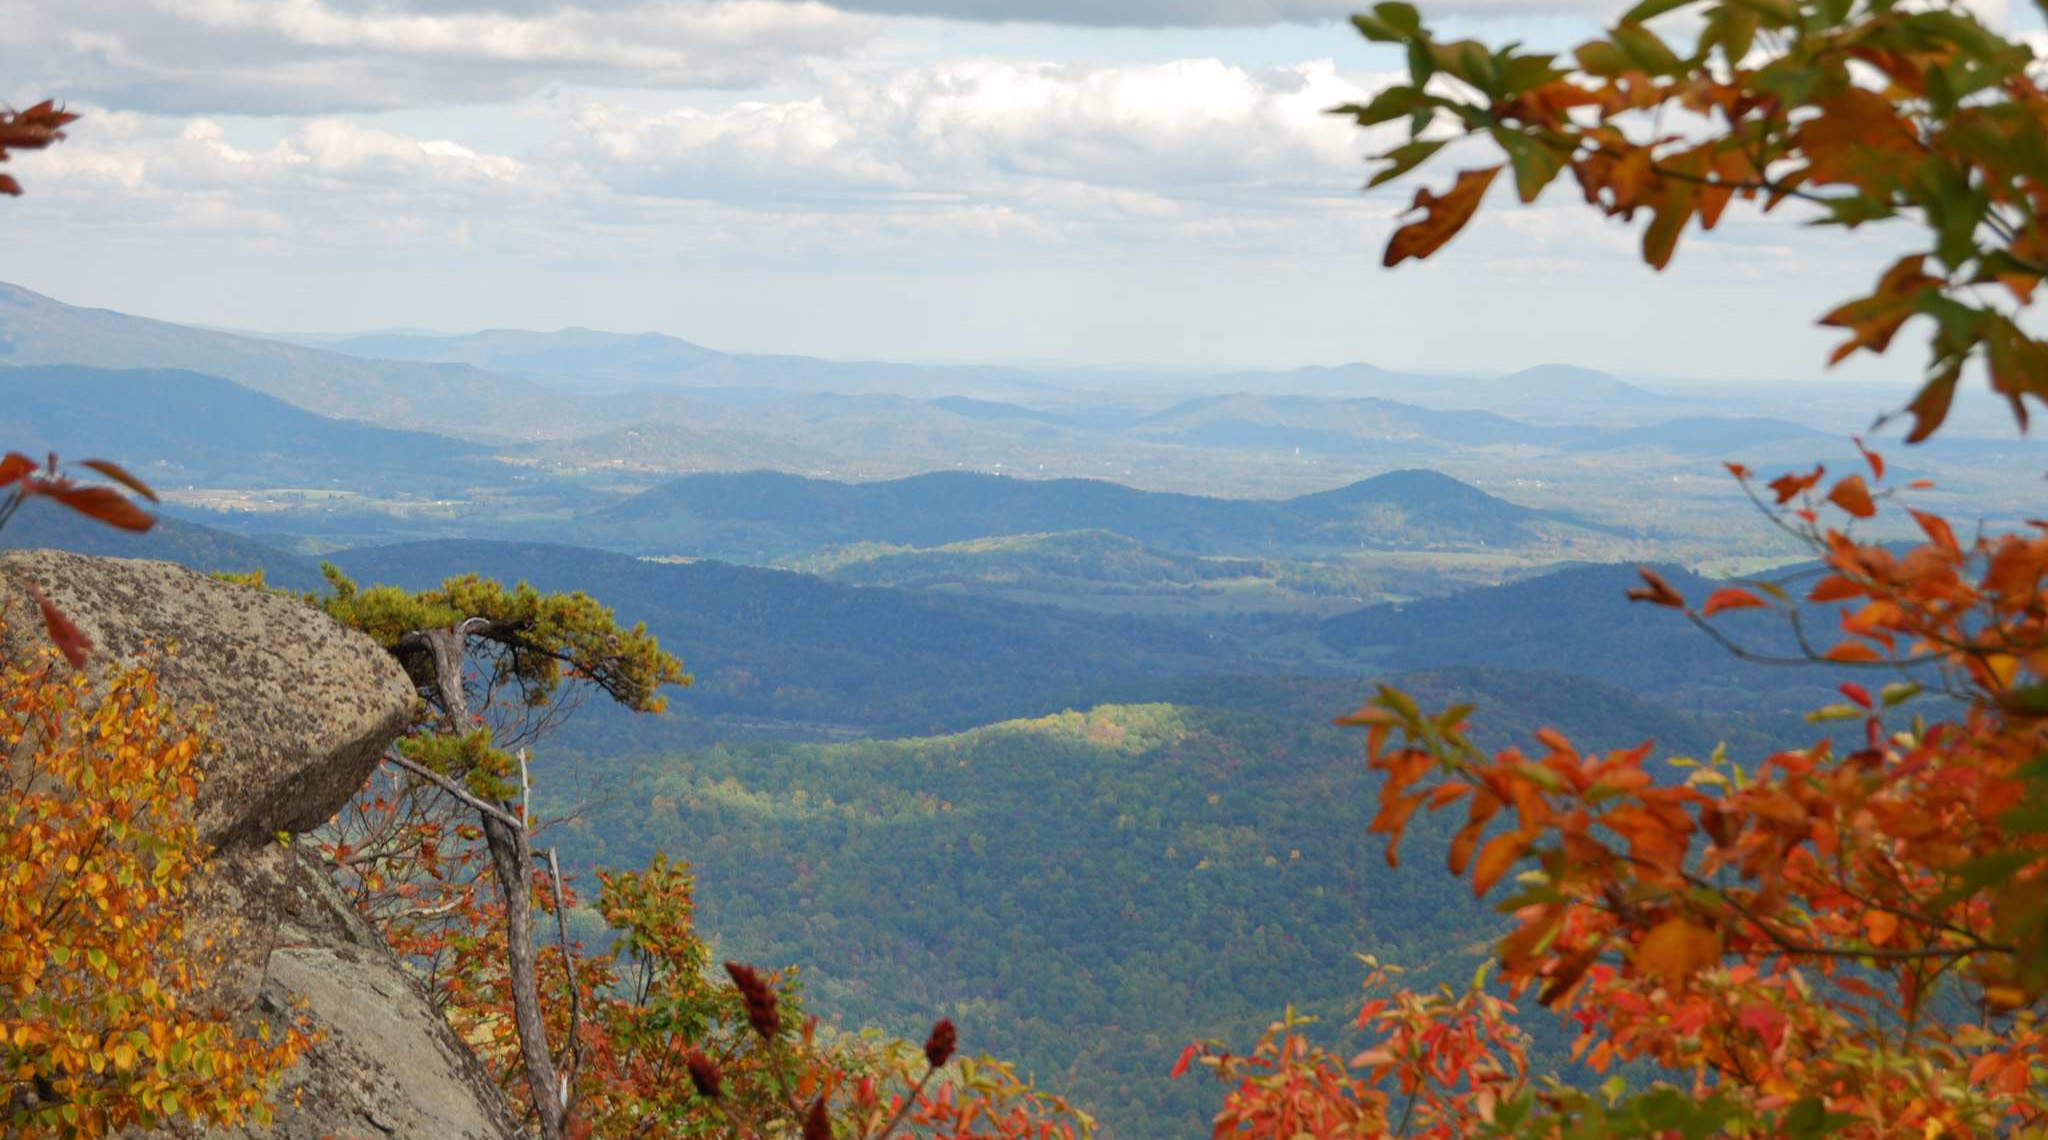
\includegraphics[width=\linewidth]{view}
% 	\caption{Wide Picture}
% 	\label{fig:view}
% \end{figure*}
%
% \begin{figure}[ht]\centering
% 	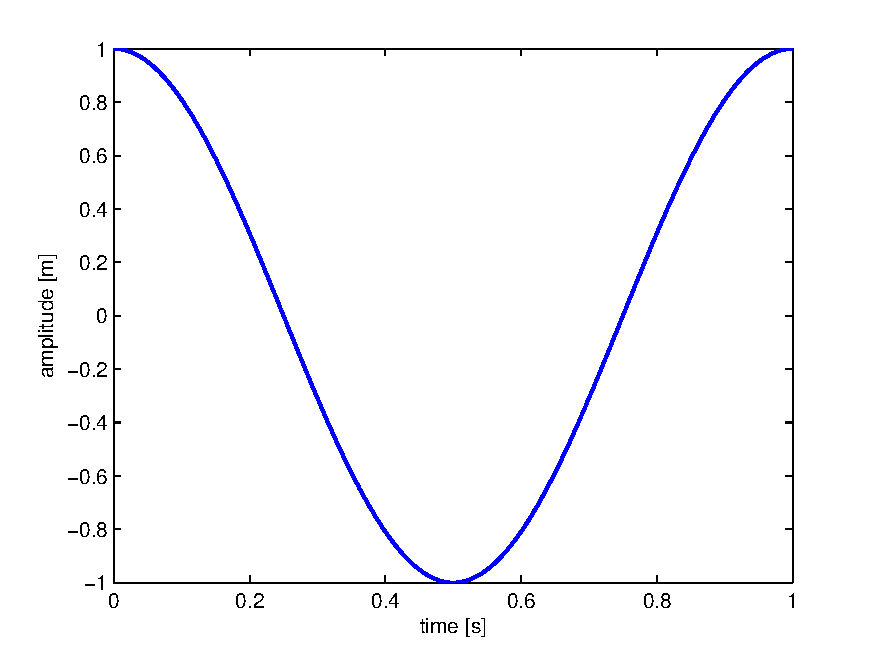
\includegraphics[width=\linewidth]{results}
% 	\caption{In-text Picture}
% 	\label{fig:results}
% \end{figure}
%
% \begin{tikzpicture}
%     % Axes
%     \draw[->] (0,0) -- (5.5,0) node[right] {V (Volume)};
%     \draw[->] (0,0) -- (0,4.5) node[above] {P (Pressure)};
%
%     % Curve y = sqrt(4x)
%     \draw[thick, blue, domain=0.5:4.5, smooth, variable=\x] 
%         plot ({\x}, {(4*\x)^(1/2)}) 
%         node[right] {$y = \sqrt{4x}$};
%
%     % Curve for backward path y = sqrt(4x)
%     \draw[thick, blue, domain=4.5:0.5, smooth, variable=\x] 
%         plot ({\x}, {(4*\x)^(1/2)});
%
%     % Shade the area under the curve (forward and backward)
%     \fill[blue!20, opacity=0.7] (0.5,0) -- plot[domain=0.5:4.5] 
%         ({\x}, {(4*\x)^(1/2)}) -- (4.5,0) -- cycle;
%
%     \fill[blue!20, opacity=0.7] (4.5,0) -- plot[domain=4.5:0.5] 
%         ({\x}, {(4*\x)^(1/2)}) -- (0.5,0) -- cycle;
%
%     % Labels for work (PdV)
%     \node[align=center] at (2.5,1.5) {$w = \int_i^f P dV + \int_f^i P dV$};
%     \node[align=left] at (0.5,1.75) {$i$};
%     \node[align=right] at (4.5,1.75) {$f$};
% \end{tikzpicture}
%
%
% \begin{tikzpicture}
%   % Define constants
%   \def\xmax{3}
%   \def\ymax{3}
%   \def\T{1.2}
%   \def\xa{0.2*\xmax}
%   \def\xb{0.8*\xmax}
%   \def\ya{\T/\xa}
%   \def\yb{\T/\xb}
%
%   % Define coordinates
%   \coordinate (A) at (\xa,\ya);
%   \coordinate (B) at (\xb,\yb);
%
%   % Draw the isotherm curve
%   \draw[myred, very thick, samples=50, domain=\xa:\xb]
%     plot (\x, {\T/\x}) 
%     node[right] {$T$};
%
%   % Fill the area under the curve and close the loop
%   \fill[mylightblue, opacity=0.5]
%     (\xa,0) -- plot[domain=\xa:\xb] (\x, {\T/\x}) -- (\xb,0) -- cycle;
%
%   % Draw the lines to close the curve
%   %\draw[thick] (\xa,0) -- (A);
%   %\draw[thick] (B) -- (\xb,0);
%
%   % Mark the points
%   %\fill (A) circle (2pt) node[right] {$P_1$, $V_1$};
%   %\fill (B) circle (2pt) node[right] {$P_2$, $V_2$};
%

%   \draw[->, thick] (0, -0.1*\ymax) -- (0, \ymax) node[anchor=north east] {$P$};
%   \draw[->, thick] (-0.1*\xmax, 0) -- (\xmax, 0) node[anchor=north east] {$V$};
% \end{tikzpicture}
%
%
%%%%%%%%%%%%%%%%%%%%%%%
% % PV diagram - constant P
% \def\N{40} % number of plot samples
% \def\xmax{3}
% \def\ymax{2.5}
% \begin{tikzpicture}
%
%   % AREA
%   \coordinate (A) at (.2*\xmax,.8*\ymax);
%   \coordinate (B) at (.8*\xmax,.8*\ymax);
%   \coordinate (C) at (.8*\xmax,.2*\ymax);
%   \fill[mylightblue] (A) rectangle (C|-0,0) node[midway,blue] {$W$};
%
%   % LINE
%   \draw[very thick,midarr=.55,myred] (A) -- (B);
%   \draw[very thick,midarr=.55,blue] (B) -- (C);
%   \fill (A) circle(0.07) node[right=5,above=2] {$P_1$, $V_1$};
%   \fill (B) circle(0.07);
%   \fill (C) circle(0.07) node[right=2] {$P_2$, $V_2$};
%
%   % AXIS
%   \draw[->,thick] (0,-0.1*\ymax) -- (0,\ymax) node[anchor=north east] {$P$};
%   \draw[->,thick] (-0.1*\xmax,0) -- (\xmax,0) node[anchor=north east] {$V$};
%
% \end{tikzpicture}
%
% % PV diagram - different heat paths
% \def\isotherm#1#2{{ #2/(#1) }}
% \begin{tikzpicture}
%   \def\Th{2.7}
%   \def\Tc{.85}
%   \coordinate (A) at ({0.30*\xmax},{\isotherm{0.30*\xmax}{\Tc}});
%   \coordinate (B) at ({0.29*\xmax},{\isotherm{0.29*\xmax}{\Th}});
%   \coordinate (C) at ({0.58*\xmax},{\isotherm{0.58*\xmax}{\Th}});
%   \coordinate (D) at ({0.82*\xmax},{\isotherm{0.82*\xmax}{\Th}});
%
%   % AXIS
%   \draw[->,thick] (0,-0.1*\ymax) -- (0,\ymax+0.1)
%     node[anchor=north east,inner sep=4,scale=1] {$P$};
%   \draw[->,thick] (-0.1*\xmax,0) -- (\xmax+0.1,0)
%     node[anchor=north east,inner sep=4,scale=1] {$V$};
%
%   % ISOTHERMS
%   \draw[mydarkblue,thick,
%         domain={\isotherm{\ymax}{\Th}}:{.95*\xmax},samples=\N,smooth]
%     plot (\x,\isotherm{\x}{\Th});
%   \draw[mydarkblue,thick,
%         domain={\isotherm{\ymax}{\Tc}}:{.95*\xmax},samples=\N,smooth]
%     plot (\x,\isotherm{\x}{\Tc});
%
%   % PATHS
%   \draw[mydarkred,thick,midarr=.5] (A) to[out=100,in=-95] (B);
%   \draw[mydarkred,thick,midarr=.6] (A) to[out=50,in=-170] (C);
%   \draw[mydarkred,thick,midarr=.5] (A) to[out=10,in=175] (D);
%   \path (A) -- (B) node[mydarkred,scale=0.9,pos=0.70,left=-1] {$Q_1$};
%   \path (A) -- (C) node[mydarkred,scale=0.9,pos=0.40,above=4] {$Q_2$};
%   \path (A) -- (D) node[mydarkred,scale=0.9,pos=0.60,below=-3] {$Q_3$};
%
%   % POINTS
%   \node[mydarkblue,above=2,right=-5,scale=0.9]
%     at (\xmax,{\isotherm{\xmax}{\Th}}) {$T+\Delta T$};
%   \node[mydarkblue,above=1,right=-5,scale=0.9]
%     at (\xmax,{\isotherm{\xmax}{\Tc}}) {$T$};
%   \fill[mydarkblue]
%      (A) circle(0.05)
%      (B) circle(0.05)
%      (C) circle(0.05)
%      (D) circle(0.05); % node[right=5,above right=-2,scale=0.9] {$P_2$, $V_2$};
%
% \end{tikzpicture}
%
% % PV diagram - isotherm
% \begin{tikzpicture}
%   \def\isotherm{(A) to[out=-60,in=170] (B)}
%   \def\T{1.2}
%   \def\xa{.2*\xmax}
%   \def\xb{.8*\xmax}
%   \def\ya{{\T/(\xa)}}
%   \def\yb{{\T/(\xb)}}
%
%   % AREA
%   \coordinate (A) at (\xa,\ya);
%   \coordinate (B) at (\xb,\yb);
%   \fill[mylightblue,samples=\N,domain=\xa:\xb]
%     plot(\x,{\T/\x}) -- (B|-0,0) -- (A|-0,0) node[midway,left=4,above=5,blue] {$W$} -- cycle;
%
%   % LINE
%   \draw[myred,very thick,midarr=.58,samples=\N,domain={\xa}:{\xb}]
%     plot(\x,{\T/\x});
%   \fill (A) circle(0.07) node[right=5,above=2] {$P_1$, $V_1$};
%   \fill (B) circle(0.07) node[right=2] {$P_2$, $V_2$};
%
%   % AXIS
%   \draw[->,thick] (0,-0.1*\ymax) -- (0,\ymax) node[anchor=north east] {$P$};
%   \draw[->,thick] (-0.1*\xmax,0) -- (\xmax,0) node[anchor=north east] {$V$};
%
% \end{tikzpicture}
%
%
% % PV diagram - specific heat capacities
% \begin{tikzpicture}
%   \def\Th{2.6}
%   \def\Tc{.85}
%   \def\Vc{0.28*\xmax}
%   \def\Vh{\Vc*\Th/\Tc}
%   \coordinate (A) at (\Vc,{\isotherm{\Vc}{\Tc}});
%   \coordinate (B) at (\Vc,{\isotherm{\Vc}{\Th}});
%   \coordinate (C) at (\Vh,{\isotherm{\Vh}{\Th}});
%
%   % AXIS
%   \draw[->,thick] (0,-0.1*\ymax) -- (0,\ymax+0.1)
%     node[anchor=north east,inner sep=4,scale=1] {$P$};
%   \draw[->,thick] (-0.1*\xmax,0) -- (\xmax+0.1,0)
%     node[anchor=north east,inner sep=4,scale=1] {$V$};
%
%   % ISOTHERMS
%   \draw[mydarkblue,thick,
%         domain={\isotherm{\ymax}{\Th}}:{.95*\xmax},samples=\N,smooth]
%     plot (\x,\isotherm{\x}{\Th});
%   \draw[mydarkblue,thick,
%         domain={\isotherm{\ymax}{\Tc}}:{.95*\xmax},samples=\N,smooth]
%     plot (\x,\isotherm{\x}{\Tc});
%
%   % PATHS
%   \path (A) -- (B) node[mydarkred,scale=0.85,pos=0.45,left=-1.5]
%     {\contour{white}{$C_\mathrm{V}\Delta T$}};
%   \path (A) -- (C) node[mydarkred,scale=0.85,pos=0.60,below=0]
%     {$C_\mathrm{P}\Delta T$};
%   \draw[mydarkred,thick,midarr=.48] (A) -- (B);
%   \draw[mydarkred,thick,midarr=.58] (A) -- (C);
%
%   % POINTS
%   \node[mydarkblue,above=2,right=-5,scale=0.9]
%     at (\xmax,{\isotherm{\xmax}{\Th}}) {$T+\Delta T$};
%   \node[mydarkblue,above=1,right=-5,scale=0.9]
%     at (\xmax,{\isotherm{\xmax}{\Tc}}) {$T$};
%   \fill[mydarkblue]
%     (A) circle(0.05)
%     (B) circle(0.05)
%     (C) circle(0.05);
%
% \end{tikzpicture}
%%%%%%%%%%%%%%%%%%%%%%%%%%%%%%%%%%%%%%%%%%%%%%%%%%%%%%%%

%-------------------------------------------------------------------------------------
%       ACKNOWLEDGMENTS
%-------------------------------------------------------------------------------------
% %\clearpage
%
% \phantomsection
% \section*{Acknowledgments}
%
% \addcontentsline{toc}{section}{Acknowledgments} % Adds this section to the table of contents

%So long and thanks for all the fish \cite{Figueredo:2009dg, Smith:2012qr}.

%-------------------------------------------------------------------------------------
%	REFERENCE LIST
%-------------------------------------------------------------------------------------
%\clearpage

% \phantomsection
% \bibliographystyle{unsrt}
% \bibliography{sample.bib}

%-------------------------------------------------------------------------------------
\end{document}
